%%%%%%%%%%%%%%%%%%%%%%%%%%%%%%%%%%%%%%
% This is the name of the style file.
%%%%%%%%%%%%%%%%%%%%%%%%%%%%%%%%%%%%%%
%
% phd  -> for a PhD dissertation
% ms   -> for an MS thesis
% If both phd and ms are used then phd will overide.  If none are used,
% then ms will be active by default.
%
% cpyr -> generate a copyright page
% lof  -> generate List of Figures
% lot  -> generate List of Tables
\documentclass[ms,cpyr,lof,lot]{uathesis}

% Subsections in TOC
%% ONLY FOR PLANNING, NOT FOR FINAL COPY %%
%\setcounter{tocdepth}{4}
%\setcounter{secnumdepth}{4}

%
%%%%%%%%%%%%%%%%%%%%%%%%%%%%%%%%
% List of any packages you use.
%%%%%%%%%%%%%%%%%%%%%%%%%%%%%%%%
%

%% FROM REU SUMMARY


\usepackage{graphicx}
\usepackage{amsmath,amssymb}
%\usepackage{gensymb}
\usepackage{xcolor}
\usepackage{mathtools}
\usepackage{etoolbox}
\usepackage{booktabs}
\usepackage{float}
\usepackage{graphicx}
\usepackage{rotating}
\usepackage{geometry}
\usepackage{multicol}
\usepackage{caption}
\usepackage{natbib}
\usepackage{siunitx}
\usepackage[all]{nowidow}
\usepackage{listings}
\usepackage{layouts}
\usepackage{bm}
\usepackage[outdir=./eps2pdf/]{epstopdf}
\graphicspath{
  {figures/}
  {figures/goals/}
  {figures/light_data/}
  {figures/attenuation/}
  {figures/results/}
}

%%%%%%%%%%%%%%%%%%%%%%%%%%%%%%%%%%
% List of definitions you define.
%%%%%%%%%%%%%%%%%%%%%%%%%%%%%%%%%%

\setlength{\tabcolsep}{12pt}

\definecolor{commentcolor}{HTML}{752000}
\definecolor{keywordcolor}{HTML}{007520}

% Listings
\lstset{
    language=[90]Fortran,
    inputpath=../kelp/code/fortran/src,
    basicstyle=\linespread{0.8}\ttfamily,
    commentstyle=\rmfamily,
    keywordstyle=\color{commentcolor},
    commentstyle=\color{keywordcolor},
    showstringspaces=false,
    numbers=left,
    breaklines=true,
    numbersep=1em,
    frame=leftline,
    tabsize=4,
    xleftmargin=.5in,
    xrightmargin=.5in}

\DeclareMathOperator{\atantwo}{atan2}

% Domain
\newcommand\xmin{{x_{\min}}}
\newcommand\xmax{{x_{\max}}}
\newcommand\ymin{{y_{\min}}}
\newcommand\ymax{{y_{\max}}}
\newcommand\zmin{{z_{\min}}}
\newcommand\zmax{{z_{\max}}}

%% FROM GOALS
\newcommand\plotwidth{7in}

%% FROM REU SUMMARY

\newcommand{\ds}{\displaystyle}

% Define error function for math mode
\newcommand{\erf}{\mbox{erf}}
% Sign function
\newcommand{\sign}{\mbox{sign}}
\newcommand{\ceil}{\mbox{ceil}}
\newcommand{\floor}{\mbox{floor}}
% Real numbers
\newcommand\R{\mathbb{R}}
% Norm
\newcommand\norm[1]{||#1||}
% Length matrix entries
\newcommand\LL{\mathcal{L}}
% Frond population
\newcommand\FF{\mathcal{F}}

%% FROM RTE PAPER

% Natural numbers
\newcommand\NN{\mathbb{N}}
% Real numbers
\newcommand\RR{\mathbb{R}}
% Complex numbers
\newcommand\CC{\mathbb{C}}
% Curly B for basis
\newcommand\BB{\mathcal{B}}
% Curly D for diagonal dominance quantity
\newcommand\DD{\mathcal{D}}
\newcommand\QQ{\mathcal{Q}}
% Uniform Norm
\newcommand\unorm[1]{\left\lVert #1 \right\rVert_\infty}
% Inner Product
\newcommand\ip[1]{\left\langle #1 \right\rangle}
% Absolute value
\newcommand\abs[1]{\left| #1 \right|}
% Complex Conjugate
\newcommand\conj\overline
% Partial derivative
\newcommand\pd[2]{\frac{\partial #1}{\partial #2}}
% Iteration superscript w/ parentheses
\newcommand{\iter}[1]{^{(#1)}}
% Disable paragraph indentation
%\setlength{\parindent}{0pt}
% End of proof
\newcommand\qed{\hfill$\blacksquare$\hspace{0.5in}}

% Bold vectors
\renewcommand\vec\bm

\newcommand\nomega{{n_{\vec{\omega}}}}


\title{Modeling the Light Field in Macroalgae Aquaculture}
\author{Oliver Graham Evans}
\conferraldate{May}{2018}

%The following commands specify the names and titles of people that
%will appear on the signature page.
%
%These four will always be needed.
\advisor{Dr. Kevin Kreider}
\chair{Dr. Kevin Kreider}
\collegedean{Dr. Linda Subich}
\gradschdean{Dr. Chand Midha}
%
%For a PhD dissertation, specify a coadvisor and three committee
%members, or four committee members only.  For an MS thesis use either
%one coadvisor or one faculty reader, not both.
%
%Typical commands for a PhD dissertation (uncomment only 4).
%\coadvisor{Name of Coadvisor}
%\committee{Name of 1st Comm Member}
%\committee{Name of 2nd Comm Member}
%\committee{Name of 3rd Comm Member}
%\committee{Name of 4th Comm Member}
%
%Typical commands for an MS thesis (uncomment only 1).
\coadvisor{Dr. Curtis Clemons}
\facreader{Dr. Gerald Young}
%\facreader{Name of Fac Reader}

\begin{document}

\maketitle
\chapter{INTRODUCTION} \label{ch:intro}

\section{Motivation}
  Given the global rise in population, efficient and innovative resource utilization is increasingly important.
Future generations face major challenges regarding food, energy, and water security while addressing major issues associated with global climate change.
Growing concern for the negative environmental impacts of petroleum-based fuel is generating a market for biofuel, especially corn-based ethanol.
However, corn-based ethanol has been heavily criticized for diverting land usage away from food production, for increasing use of fertilizers that impair water quality, and for low return on energy investments for production.
At the same time, a great deal of unutilized saltwater coastline is available for both food and fuel production through seaweed cultivation.
Specifically, the sugar kelp \textit{Saccharina latissima} is known to be a viable source of food,  both for direct human consumption and biofuel production.

%TODO: Nitrogen concerns, wastewater treatment.
Nitrogen leakage into water bodies is a significant ecological problem, and is especially relevant near large conventional agriculture facilities due to run-off from nitrogen-based fertilizers, as well as near wastewater treatment plants.
Waste water treatment plants (WWTPs) in particular are facing increasingly stringent regulation of nutrients in their effluent discharges from the US Environmental Protection Agency (USEPA) and state regulatory agencies.
Nutrient management at WWTPs requires significant infrastructure, operations, and maintenance investments for tertiary treatment processes. Many treatment works are constrained financially or by space limitations in their ability to expand their treatment works.
As an alternative to conventional nutrient remediation techniques, the cultivation of the macroalgae \textit{Saccharina latissima} (sugar kelp) within the nutrient plume of WWTP ocean outfalls has been proposed.
The purpose of such an undertaking would be twofold: to prevent eutrophication of the surrounding ecosystem by sequestering nutrients, and to provide supplemental nutrients that benefit macroalgae cultivation. %TODO: Cite

Large scale macroalgae cultivation has long existed in Eastern Asia due to the popularity of seaweed in Asian cuisine, and low labor costs that facilitate its manual seeding and harvest.
  More recently, less labor-intense and more industrialized kelp aquaculture has been developing in Scandinavia and in the Northeastern United States and Canada.
For example, the MACROSEA project is a four year international research collaboration led by SINTEF, an independent research organization in Norway, and funded by the Research Council of Norway targeting ``successful and predictable production of high quality biomass thereby making significant steps towards industrial macroalgae cultivation in Norway.'' %TODO: Cite this
The project includes both cultivators and scientists, working to develop a precise understanding of the full life cycle of kelp and its interaction with its environment.
A fundamental aspect of this endeavor is the development of mathematical models to describe the growth of kelp.

Recently, a growth model\cite{broch_modelling_2012} for S. latissima has been produced and integrated into the SINMOD\cite{wassmann_modelling_2006} hydrodynamic and ecosystem model of SINTEF.
One aspect of the model which has yet to be fully developed is the availability of light, considering factors such as absorption and scattering by the aquatic medium, as well as by the kelp itself.
This thesis contributes to this effort by developing a first-principles model of the light field in a kelp farming environment.
As a first step, a model for the spatial distribution of kelp is developed.
Radiative transfer theory is then applied to determine the effects of the kelp and water on the availability of light throughout the medium.
A finite difference solution to the radiative transfer equation is developed, followed by asymptotic approximations that prove to be sufficiently accurate for clear water, and significantly less computationally intensive.
A detailed description of the numerical solution of this model is presented, accompanied by source code for a FORTRAN implementation of the solution.
This model can be used independently, or in conjunction with a kelp growth model to determine the amount of light available for photosynthesis at a single time step.

\begin{figure}[h]
  \centering
  \includegraphics[width=0.5\textwidth]{kelp_photo/sonja}
  \caption{\textit{Saccharina latissima} being harvested}
  % https://blogs.qub.ac.uk/qubio/files/2016/04/H5-5.jpg
  %TODO: Cite properly or replace with photo from Shane
\end{figure}


\section{Background on Kelp Models}

Mathematical modeling of macroalgae growth is not a new topic, although it is a reemerging one.
Several authors in the second half of the twentieth century were interested in describing the growth and composition of the macroalgae \textit{Macrocystis pyrifera}, commonly known as ``giant kelp,'' which grows prolifically off the coast of southern California.
The first such mathematical model was developed by W.J. North for the Kelp Habitat Improvement Project at the California Institute of Technology in 1968 using seven variables.
By 1974, Nick Anderson greatly expanded on North's work, and created the first comprehensive model of kelp growth which he programmed using FORTRAN\cite{anderson_mathematical_1974}.
In his model, he accounts for solar radiation intensity as a function of time of year and time of day, and refraction on the surface of the water.
He uses a simple model for shading, simply specifying a single parameter which determines the percentage of light that is allowed to pass through the kelp canopy floating on the surface of the water.
He also accounts for attenuation due to turbidity using Beer's Law.
Using this data on the availability of light, he calculates the photosynthesis rates and the growth experienced by the kelp.

Over a decade later in 1987, G.A.
Jackson expanded on Anderson's model for \textit{Macrocystis pyrifera}, with an emphasis on including more environmental parameters and a more complete description of the growth and decay of the kelp\cite{jackson_modelling_1987}. 
The author takes into account respiration, frond decay, and sub-canopy light attenuation due to self-shading.
Light attenuation is represented with a simple exponential model, and self-shading appears as an added term in the decay coefficient.
The author does not consider radial or angular dependence on shading. %TODO:  Check this. Was previously ambiguous.
Jackson also expands Anderson's definition of canopy shading, treating the canopy not as a single layer, but as 0, 1, or 2 discrete layers, each composed of individual fronds.
While this is a significant improvement over Anderson's light model, it is still rather simplistic.

Both Anderson's and Jackson's model were carried out by numerically solving a system of differential equations over small time intervals.
In 1990, M.A. Burgman and V.A. Gerard developed a stochastic population model\cite{burgman_stage-structured_1990}.
This approach is quite different, and functions by dividing kelp plants into groups based on size and age and generating random numbers to determine how the population distribution over these groups changes over time based on measured rates of growth, death, decay, light availability, etc.
In the same year, Nyman et. al. published a similar model alongside a Markov chain model, and compared the results with experimental data collected in New Zealand\cite{nyman_macrocystis_1990}.

In 1996 and 1998 respectively, P. Duarte and J.G. Ferreira used the size-class approach to create a more general model of macroalgae growth, and Yoshimori et. al. created a differential equation model of \textit{Laminaria religiosa} with specific emphasis on temperature dependence of growth rate\cite{duarte_model_1997,yoshimori_mathematical_1998}.
These were the some of the first models of kelp growth that did not specifically relate to \textit{Macrocystis pyrifera} (``giant kelp''). 
Initially, there was a great deal of excitement about this species due to it's incredible size and growth rate, but difficulties in harvesting and negative environmental impacts have caused scientists to investigate other kelp species. % TODO: Cite

\section{Background on Radiative Transfer}
In terms of optical quantities, of primary interest is in the radiance at each point from all directions, which affects the photosynthetic rate of the kelp, and therefore the total amount of biomass producible in a given area as well as the total nutrient remediation potential.
The equation governing the radiance throughout the system is known as the radiative transfer equation (RTE), which has been largely unutilized in the fields of oceanography and aquaculture.
The radiative transfer equation has been used primarily in stellar astrophysics; it's application to marine biology is fairly recent\cite{mobley_radiative_2001}.
In its full form, radiance is a function of 3 spatial dimensions, 2 angular dimensions, and frequency, making for an incredibly complex problem. % TODO: Cite?
In this work, frequency is ignored, only monochromatic radiation is considered.
The RTE states that along a given path, radiance is decreased by absorption and scattering out of the path, while it is increased by emission and scattering into the path.
In our situation, emission is negligible, owing only perhaps to some small luminescent phytoplankton or other anomaly, and can therefore be safely ignored.

% TODO: Remove?
Understanding the growth rate and nutrient recovery by
kelp cultures has important marine biological implications. For example, recent
work by our research group at Clarkson University, the University of Maine, and
SINTEF Fisheries and Aquaculture is investigating kelp aquaculture as a means to
recover nutrients from wastewater effluent plumes in coastal environments into a
valuable biomass feedstock for many products. Current models for kelp growth
place little emphasis on the way in which nearby plants shade one another.
Self-shading may be a significant model feature, though, as light availability
may impact the growth and composition of the kelp biomass, and thus the mixture
of goods that may be derived.

\section{Overview of Thesis}
% TODO: Check for redundancy
The remainder of this document is organized as follows.
In Chapter \ref{chap:kelp}, probabilistic model is developed to describe the spatial distribution of kelp by assuming simple distributions for the lengths and orientations of fronds.
Chapter \ref{chap:light} begins with a survey of fundamental radiometric quantities and optical properties of matter.
The spatial kelp distribution from Chapter \ref{chap:kelp} is used to determine optical properties of the combined water-kelp medium,
and the radiative transfer equation, an integro-partial differential equation which describes the the light field as a function of position and angle, is discussed.
An asymptotic expansion is explored for cases where absorption dominates scattering in the medium, such as in very clear water or high kelp density.
In Chapter \ref{chap:numerical}, details are given for the numerical solution of the equations from Chapters \ref{chap:kelp} and \ref{chap:light}.
Both the full finite difference solution and the asymptotic approximation are described.
Next, in Chapter \ref{chap:parameters}, the availability of necessary parameters in the literature is discussed.
For those which are not readily available, give rough estimates are given or describe experimental methods for their determination are described.
Then, in Chapter \ref{chap:model_analysis}, necessary grid resolution for adequate accuracy in the full finite difference solution is determined.
The finite difference solution is compared to the asymptotic approximation for a few sets of optical properties.
Further, we showcase the effect of varying a few key parameters on the light field predicted by the asymptotic approximation.
Afterwards, the light model developed here is used in a numerical simulation of kelp growth, and the predicted light field and biomass production are compared to those predicted by a simpler 1D exponential decay light model.
Finally, Chapter \ref{chap:conclusion} concludes the thesis by giving a brief summary of the model, discuss and its performance, and suggest improvements and avenues for future work.

\chapter{KELP MODEL}
\label{chap:kelp}

In order to properly model the spatial distribution of light around the kelp, it is first necessary to formulate a spatial description of the kelp.
Probability distributions are given for the size and orientation of the individual kelp fronds, which are inverted to determine the probability of a point in space being occupied by kelp.
Ultimately, the kelp density at any point in space is calculated, which informs the absorption coefficient of the effective kelp--water medium.


\section{Physical Setup}
The life of cultivated macroalgae generally begins in the laboratory, where microscopic kelp spores are inoculated onto a thread in a small laboratory pool.
This thread is wrapped around a larger rope as in Figure \ref{fig:rope_thread}, which is hung from buoys in the ocean.
The two primary configurations are vertical and horizontal or ``long'' lines.
In the case of vertical lines, the seaweed rope hangs straight down from a single buoy, and is either weighted or anchored.
In the case of long lines, the rope is strung from one buoy to another.
Long lines allow more light to reach the seaweed since it grows closer to the surface, but more vertical lines can be set up in a given area,
which may be advantageous for IMTA.

\begin{figure}[H]
  \centering
  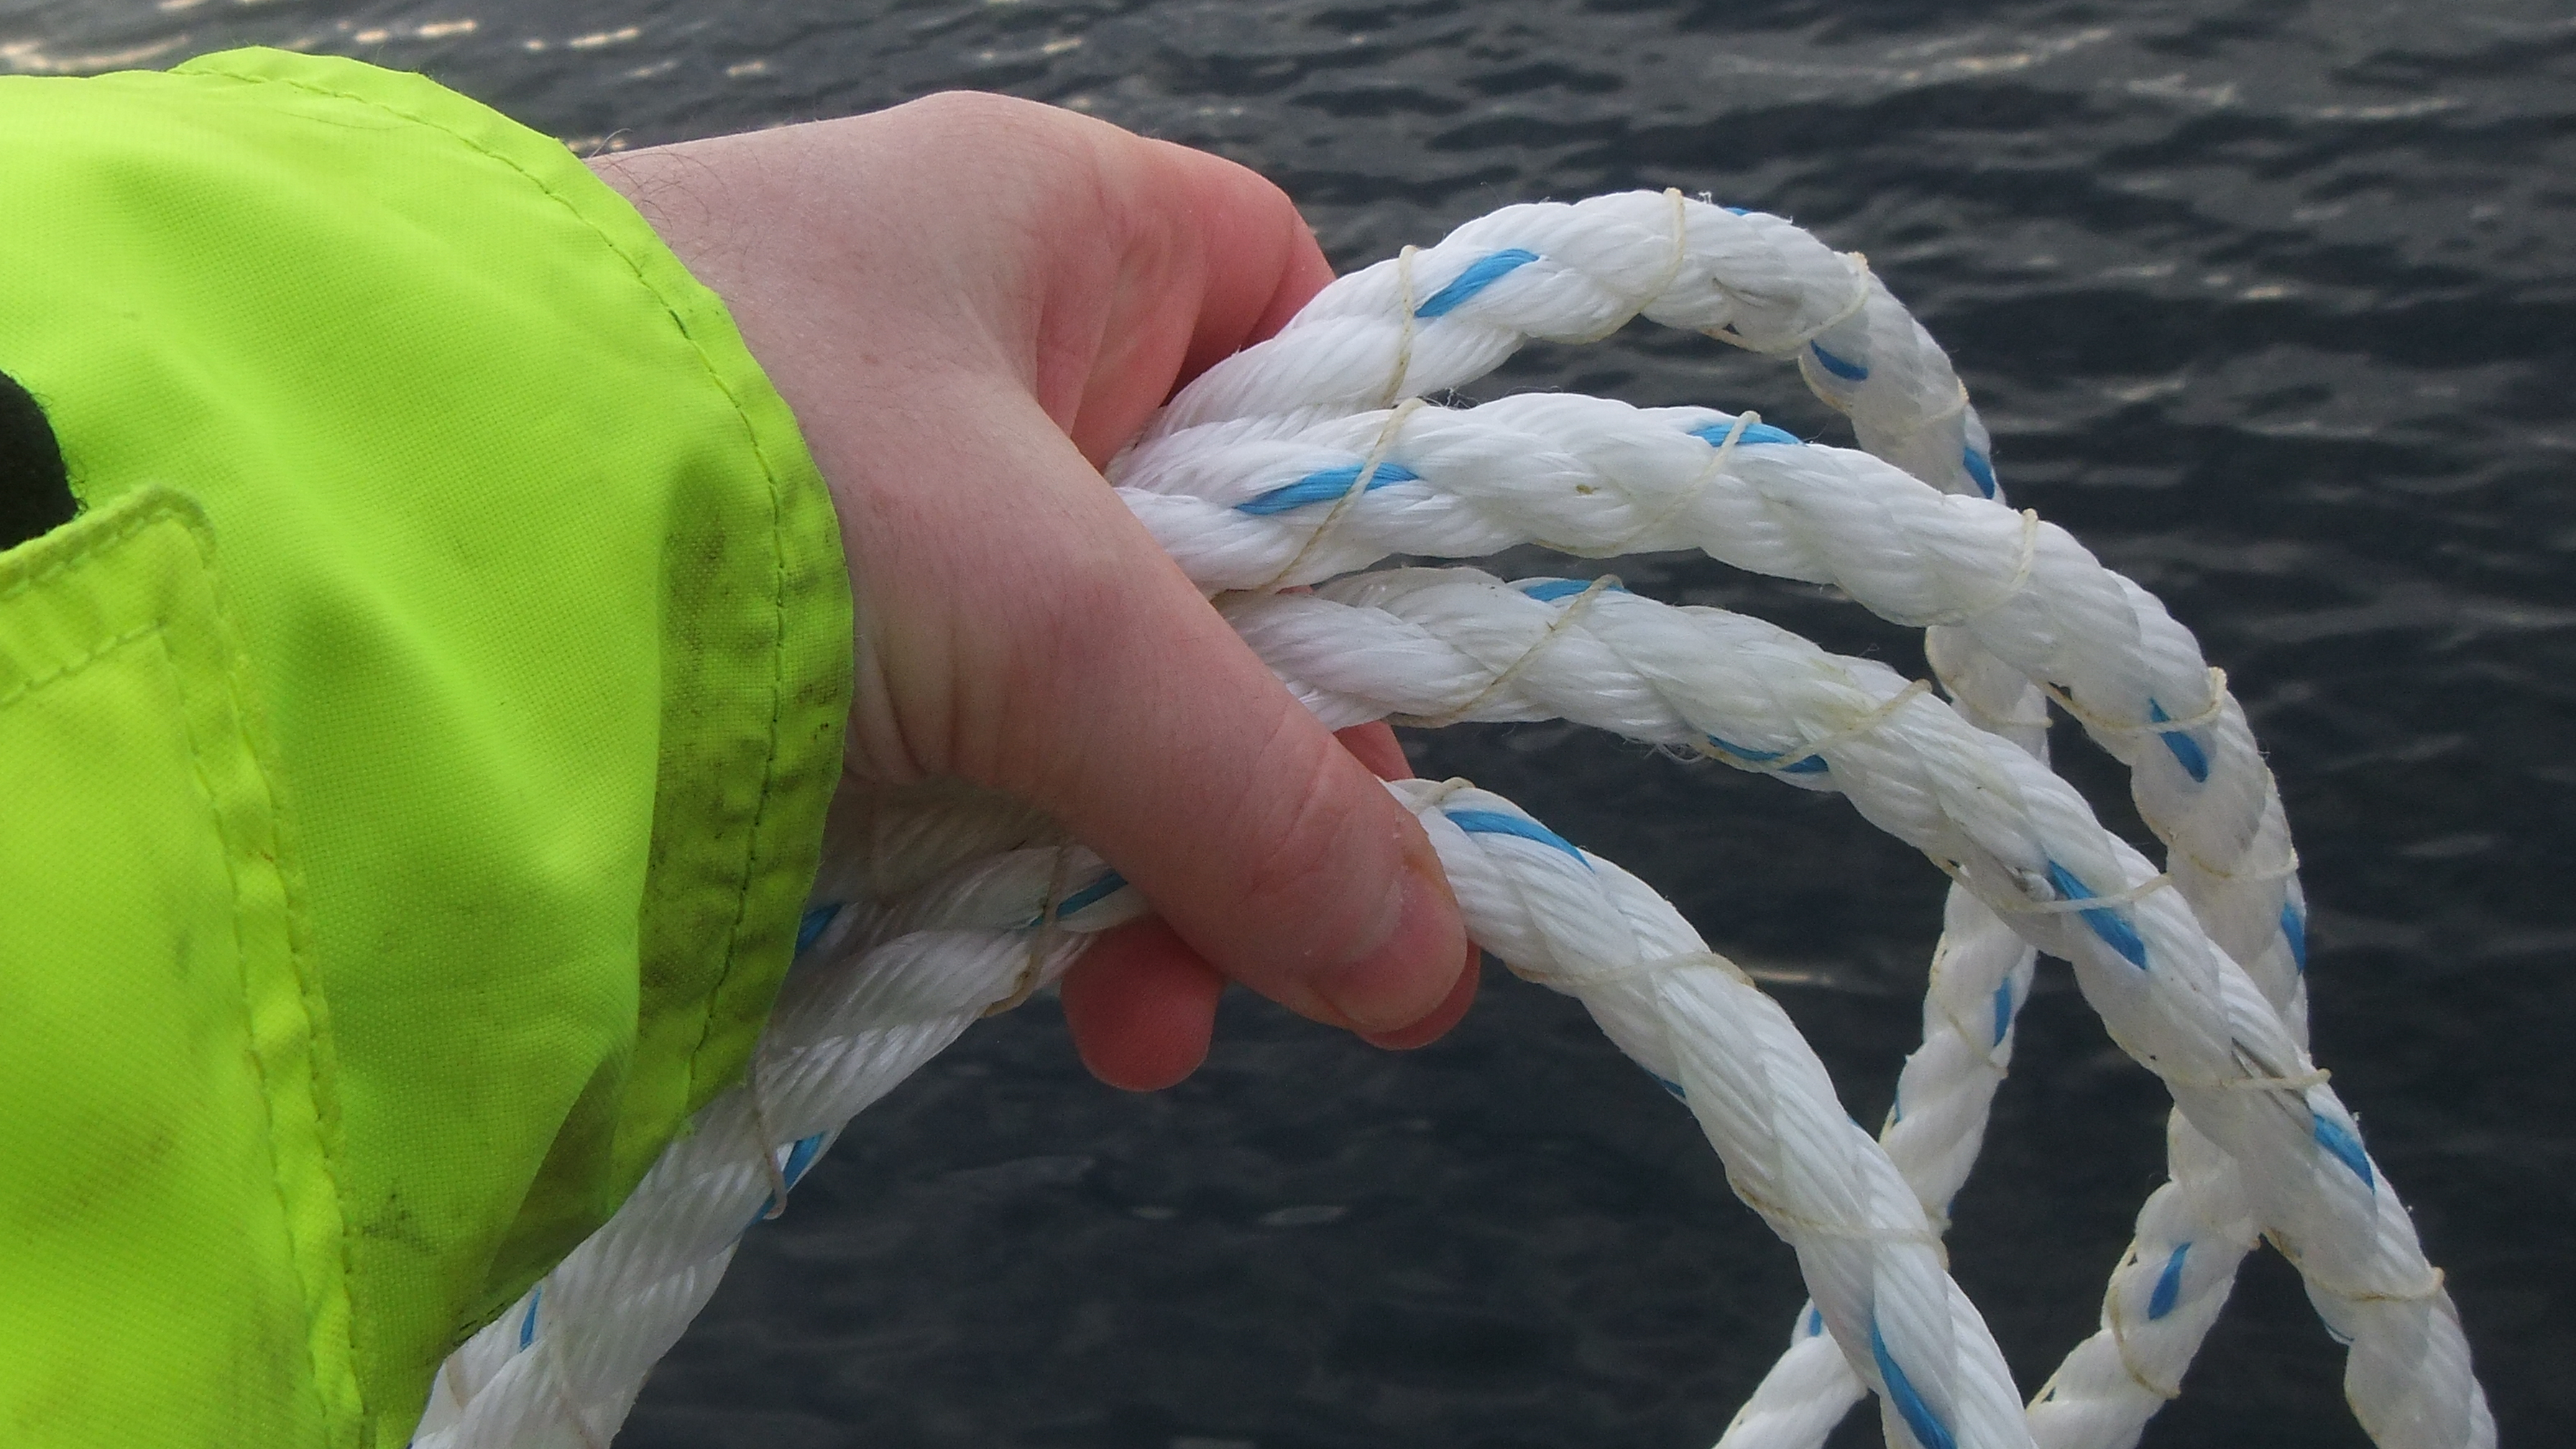
\includegraphics[width=0.65\textwidth]{kelp_photo/rope_thread}
  \caption{\textit{Saccharina latissima} innoculated onto a thread wrapped around a rope on which it is to be grown.}
  \label{fig:rope_thread}
\end{figure}

We consider only the case of a rigid vertical rope which does not sway in the current.
The mature \textit{Saccharina latissima} plant consists of a single frond (leaf), a stipe (stem) and a holdfast (root structure).
For the sake of this model, only the kelp frond is considered, and its base is attached directly to the rope.
The ``gentle undulation approximation'' is employed, whereby the fronds are modeled as perfectly horizontal.
While at any given time they may point up or down due to water current and gravity, we consider the horizontal
state to be an average configuration.
This simplification allows for the three-dimensionally distributed population of kelp fronds
to be considered a collection of independent populations in two-dimensional depth layers.
A computer rendering of this scenario is shown in Figure \ref{fig:kelp_array}.

\begin{figure}[H]
	\centering
	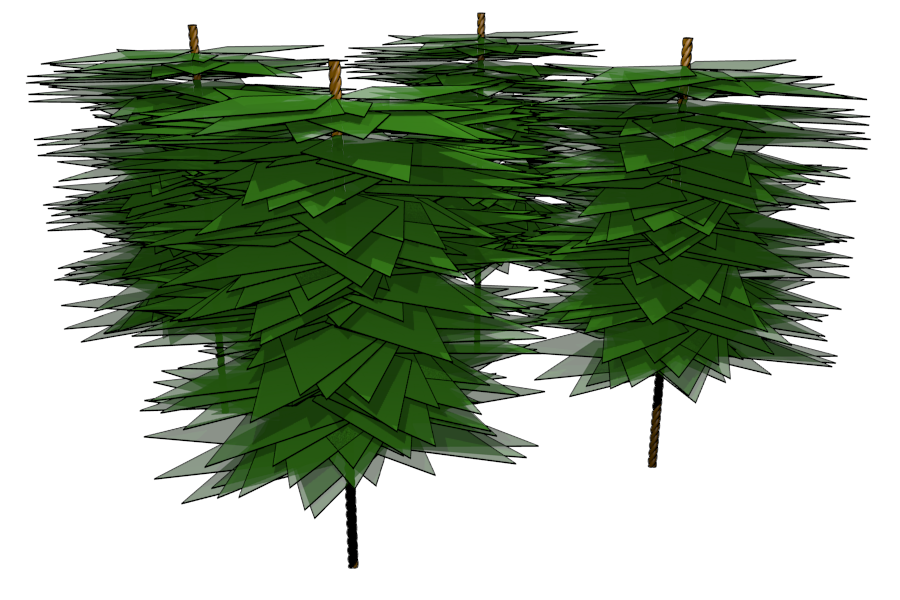
\includegraphics[width=3.5in]{kelp_array}
	\captionof{figure}{Rendering of four nearby vertical kelp ropes as represented in the spatial distribution model. Note the kite--shaped fronds and horizontal orientation.}
  \label{fig:kelp_array}
\end{figure}

\section{Coordinate System}
Consider the rectangular domain
\begin{align*}
  \xmin &\leq x \leq \xmax, \\
  \ymin &\leq y \leq \ymax, \\
  \zmin &\leq z \leq \zmax.
\end{align*}
For all three dimensional analysis, we use the absolute coordinate system defined in Figure \ref{fig:3dcoords}.
In the following sections, it is necessary to convert between Cartesian and spherical coordinates, which we do using the relations
\begin{equation}
  \left\{
	\begin{split}
		x & = r\sin\phi\cos\theta, \\
		y & = r\sin\phi\sin\theta, \\
		z & = r\cos\phi. \\
	\end{split}
  \right.
	\label{eqn:coords}
\end{equation}
Therefore, for some function $f(x,y,z)$, we can write its derivative along a path in spherical coordinates in terms of Cartesian coordinates using the chain rule,
\begin{equation*}
	\frac{\partial f}{\partial r}
	=\frac{\partial f}{\partial x}\frac{\partial x}{\partial r}
	+ \frac{\partial f}{\partial y}\frac{\partial y}{\partial r}
	+ \frac{\partial f}{\partial z}\frac{\partial z}{\partial r}.
\end{equation*}
Then, calculating derivatives from \eqref{eqn:coords} yields
\begin{equation}
	\frac{\partial f}{\partial r}
	=\frac{\partial f}{\partial x}\sin\phi\cos\theta
	+ \frac{\partial f}{\partial y}\sin\phi\sin\theta
	+ \frac{\partial f}{\partial z}\cos\phi.
	\label{eqn:partials}
\end{equation}
\begin{figure}[H]
	\centering
	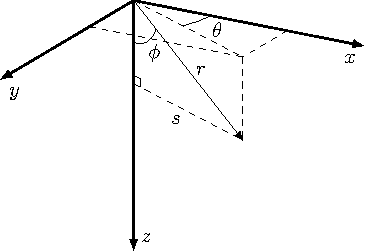
\includegraphics[width=3in]{3d_coords}
	\caption{Downward-facing right-handed coordinate system with radial distance $r$ from the origin, distance $s$ from the $z$ axis, zenith angle $\phi$ and azimuthal angle $\theta$.}
	\label{fig:3dcoords}
\end{figure}

\section{Population Distributions}
In order to construct a spatial distribution of kelp fronds, a simple kite-shaped geometry is introduced,
and frond lengths and azimuthal orientations are assumed to be distributed predictably.
Since it is assumed that fronds extend perfectly horizontally, no angular elevation distribution is required.

\subsection{Frond Shape}
\label{sec:shape}

\begin{figure}[h]
	\centering
  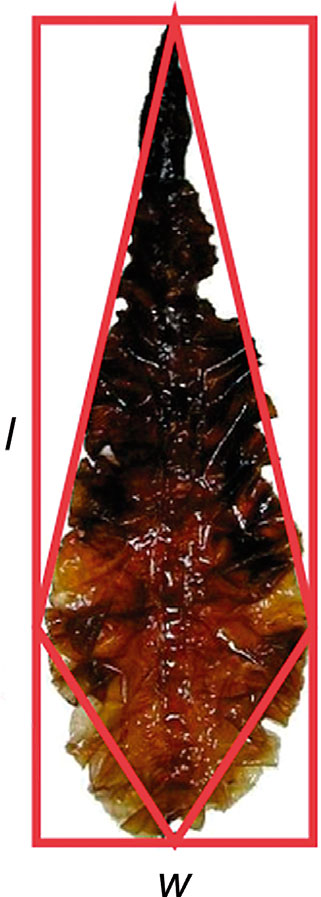
\includegraphics[width=1.2in]{kelp_photo/kite}
  %TODO: Cite this?
  \qquad
	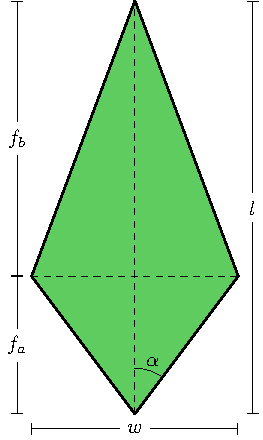
\includegraphics[width=2in]{frond}
	\captionof{figure}{Simplified kite-shaped frond.}
	\label{fig:frond}
\end{figure}

The frond is assumed to be kite-shaped with length $l$ from base to tip, and width $w$ from left to right.
In Figure \ref{fig:frond}, the base is shown at the bottom and the tip is shown at the top.
The proximal length is the shortest distance from the base to the diagonal connecting the left and right corners, and is notated as $f_a$.
Likewise, the distal length, notated $f_b$, is the shortest distance from that diagonal to the tip.
It is therefore clear that
 \begin{equation*}
	 f_a + f_b = l.
 \end{equation*}
When considering a whole population with varying sizes, it is more convenient to specify ratios than absolute lengths.
Define the ratios
\begin{align*}
	f_r &= \frac{l}{w}, \\
	f_s &= \frac{f_a}{f_b}.
\end{align*}
These ratios are assumed to be constant among the entire population, so that all fronds are geometrically similar.
Thus, the shape of the frond can be fully specified by $l$, $f_r$, and $f_s$;
it is possible to redefine $w$, $f_a$ and $f_b$ from the preceding formulas as
\begin{align*}
	w &= \frac{l}{f_r}, \\
	f_a &= \frac{lf_s}{1+f_s}, \\
	f_b &= \frac{l}{1+f_s}.
\end{align*}
The angle $\alpha$, half of the angle at the base corner, is also noteworthy.
From the above equations, it follows that
\begin{equation*}
	\alpha = \tan^{-1}\left(\frac{2f_rf_s}{1+f_s}\right).
\end{equation*}

It is useful to convert between frond length and surface area, which can be done via the relations
\begin{align}
  A &= \frac{lw}{2} = \frac{l^2}{2f_r},
  \label{eqn:area_from_length} \\
  l &= \sqrt{2Af_r}.
  \label{eqn:length_from_area}
\end{align}

\subsection{Length and Angle Distributions}
\label{sec:dist}
In any given depth layer, the distribution of frond lengths is assumed to be normal, with mean $\mu_l$ and standard deviation $\sigma_l$.
That is, it has the probability density function (PDF)
\begin{equation*}
  P_l(l) = \frac{1}{\sqrt{2\pi\sigma_l^2}}\exp\left(-\frac{(l-\mu_l)^2}{2\sigma_l^2}\right).
\end{equation*}

It is further assumed that frond orientation angle varies according to the von Mises distribution, which is the periodic analogue of the normal distribution, defined on $[-\pi,\pi]$ rather than $(-\infty,\infty)$.
The von Mises distribution has two parameters, $\mu$ and $\kappa$, which shift and sharpen its peak respectively, as shown in Figure \ref{fig:vonmises}.
$\kappa$ is analogous to $1/\sigma$ in the normal distribution.
In the absence of current, the frond angles are distributed uniformly, while as current velocity increases, they become increasingly likely to align parallel to the current, depending on the stiffness of the frond and stipe.
Assuming a linear relationship between the current velocity and the steepness of the angular distribution, define the \textit{frond alignment coefficient} $\eta$, with units of inverse velocity(\SI{}{\s\per\m}).
Then, use $\mu = \theta_w$ and $\kappa = \eta v_w$ as the von Mises distribution parameters.
Note that $\theta_w$ and $v_w$ vary over depth, while $\eta$ is assumed constant for the population.
Then, the PDF for the von Mises frond angle distribution is
\begin{equation*}
	P_{\theta_f}(\theta_f) = \frac{\exp\left(\eta v_w\cos(\theta_f-\theta_w)\right)}{2\pi I_0(\eta v_w)},
\end{equation*}
where $I_0(x)$ is the modified Bessel function of the first kind of order 0.
Notice that unlike the normal distribution, the von Mises distribution approaches a \textit{non-zero} uniform distribution as $\kappa$ approaches 0, so
\begin{equation*}
	\displaystyle \lim_{v_w \to 0}P_{\theta_f}(\theta_f) = \frac{1}{2\pi} \;\forall\, \theta_f \in [-\pi,\pi].
\end{equation*}

\begin{figure}[h]
	\centering
	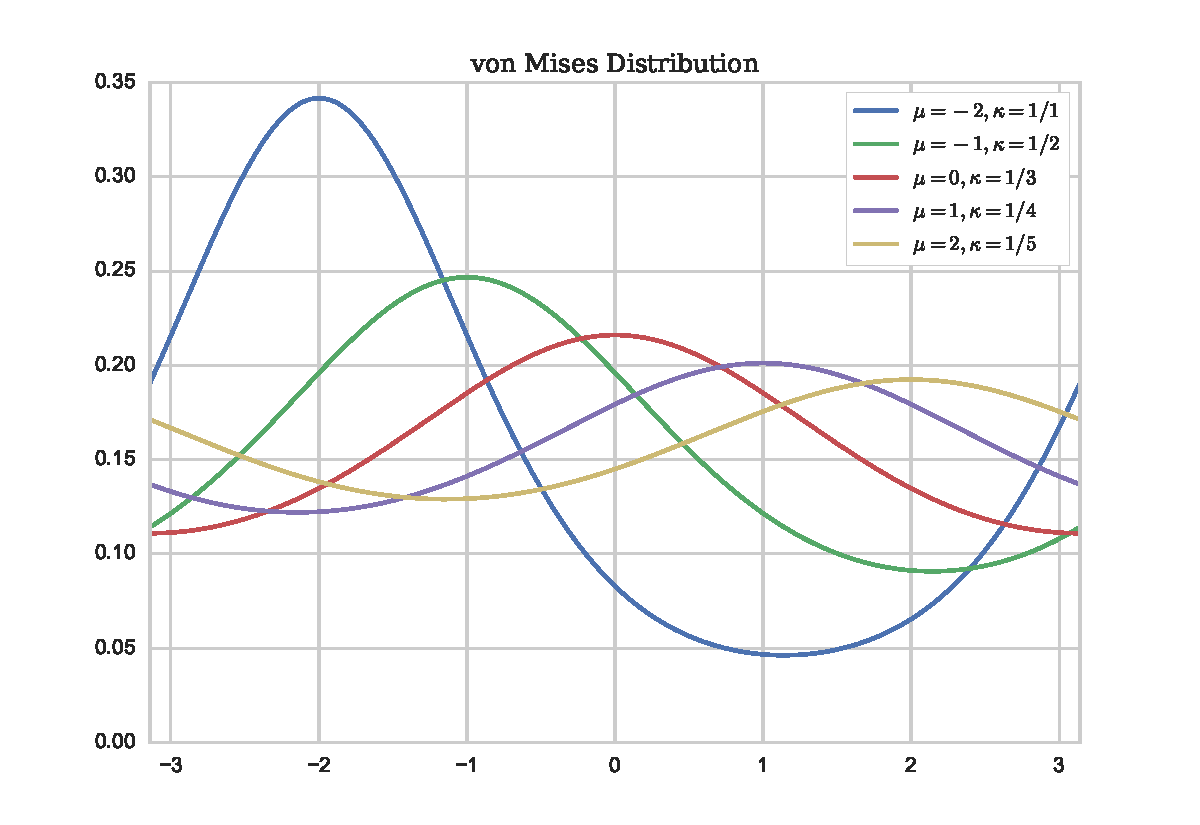
\includegraphics[width=6in]{vonmises}
	\captionof{figure}{von Mises distribution for a variety of parameters.}
	\label{fig:vonmises}
\end{figure}

\subsection{Joint Length-Orientation Distribution}
\label{sec:dist_2d}
The previous two distributions can reasonably be assumed to be independent of one another. That is, the angle of the frond does not depend on the length, or vice versa.
Therefore, the probability of a frond simultaneously having a given frond length and angle is the product of their individual probabilities.
Given independent events $A$ and $B$, the probability of their intersection is the product of their individual probabilities.
That is,
\begin{equation*}
	\label{eqn:ind_prob}
	P(A \cap B) = P(A)P(B).
\end{equation*}
Then the probability of frond length $l$ and frond angle $\theta_f$ coinciding is
\begin{equation}
  \label{eqn:p2d}
	P_{2D}(\theta_f,l) = P_{\theta_f}(\theta_f) \cdot P_l(l).
\end{equation}
A contour plot of this 2D distribution for a specific set of parameters is shown in Figure \ref{fig:dist_2d}, where probability is represented by color in the 2D plane.
Darker green represents higher probability, while lighter beige represents lower probability.
In Figure \ref{fig:kelp_sample}, 50 samples are drawn from this distribution and plotted.

It is important to note that if $P_{\theta_f}$ were dependent on $l$, the above definition of $P_{2D}$ would no longer be valid.
For example, it might be more realistic to say that larger fronds are less likely to bend towards the direction of the current.
In this case, \eqref{eqn:ind_prob} would no longer hold, and it would be necessary to use the more general Bayes' Theorem
\begin{equation*}
	P(A \cap B) = P(A)P(B|A) = P(B)P(B|A),
\end{equation*}
which is currently not taken into consideration in this model.

\begin{figure}[h]
	\centering
	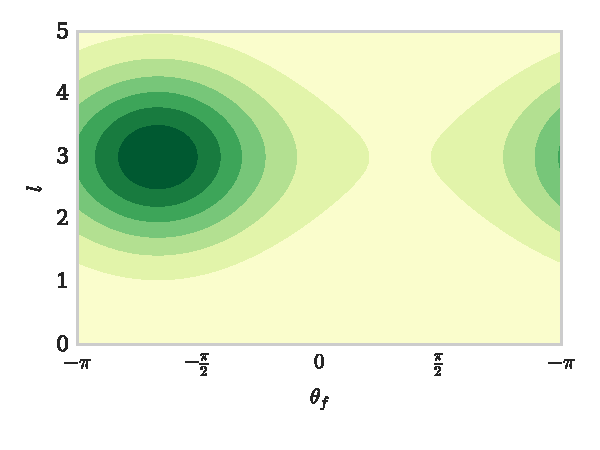
\includegraphics[width=4.5in]{prob_2d}
	\captionof{figure}{2D length-angle probability distribution with $\theta_w=7\pi/4$, $v_w=1$, $\mu_l=3$, $\sigma_l=1$.}
	\label{fig:dist_2d}
\end{figure}

\begin{figure}[h]
	\centering
	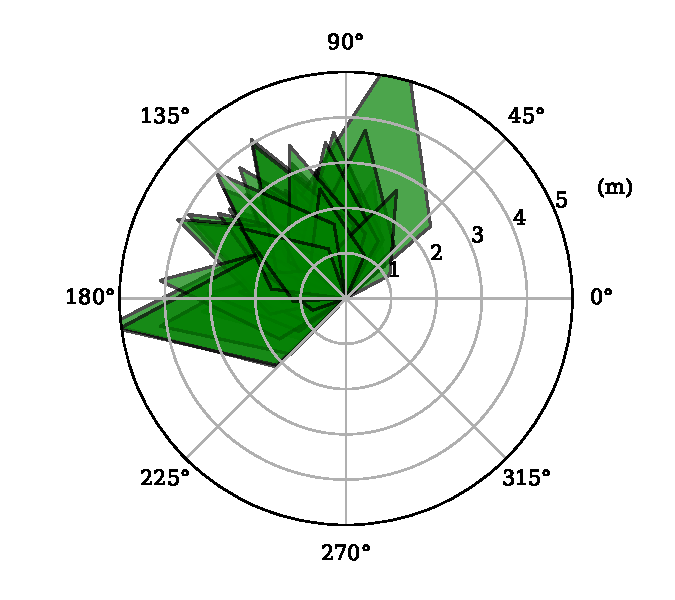
\includegraphics[width=4.5in]{kelp_sample}
	\captionof{figure}{A sample of 50 kelp fronds with shape parameters $f_s=0.5$ and $f_r=2$ whose lengths are picked from a normal distribution and whose angles are picked from a von Mises distribution.}
	\label{fig:kelp_sample}
\end{figure}

\section{Spatial Distribution}
In this section, the population length and angle distributions from the previous section are used to construct a spatial distribution of kelp.
This is made possible by the simple kite-shape fronds, and would be considerably more difficult with more general frond shapes.
\subsection{Rotated Coordinate System}
\label{sec:rot_coords}
To determine under what conditions a frond will occupy a given point, we begin by
describing the shape of the frond in Cartesian coordinates and then convert to polar coordinates.
Of primary interest are the edges connected to the frond tip.
For convenience, we will use a rotated polar coordinate system $(\theta',s)$ such that the line connecting the base to the tip points in the $+y$ direction ($\theta=\pi/2$), with the base at $(0,0)$.
Denote the Cartesian analogue of this coordinate system as $(x',y')$ which is related to $(\theta',s)$ by
\begin{align*}
	x' &= s\cos\theta' \\
	y' &= s\sin\theta' \\
	s &= \sqrt{x'^2+y'^2}, \\
	\theta' &= \atantwo(y, x).
\end{align*}

\subsection{Functional Description of Frond Edge}
With this coordinate system established, the outer two edges of the frond can be described in Cartesian coordinates as a piecewise linear function connecting the left corner: $(-w/2,f_a)$, the tip: $(0,l)$, and the right corner: $(w/2,f_a)$.
This function has the form
\begin{equation*}
	y'_f(x') = l-\sign(x')\frac{f_b}{w/2}x'.
\end{equation*}
Using the equations in Section \ref{sec:rot_coords}, this can be written in polar coordinates after some rearrangement as
\begin{equation*}
	s_f'(\theta';l) = \frac{l}{\sin\theta' + S(\theta')\frac{2f_b}{w}\cos\theta'},
\end{equation*}
where
\begin{equation*}
	S(\theta') = \sign(\cos\theta').
\end{equation*}
Then, using the relationships in Section \ref{sec:shape}, the above equation can be rewritten in terms of the frond ratios $f_s$ and $f_r$ as
\begin{equation}
	\label{eqn:rf_rel}
	s_f'(\theta';l) = \frac{l}{\sin\theta' + S(\theta')\frac{2f_r}{1+f_s}\cos\theta'}.
\end{equation}
For convenience, denote the denominator of \eqref{eqn:rf_rel} as $d_f'(\theta')$.
To generalize to a frond pointed at an angle $\theta_f$, we introduce the coordinate system $(\theta,s)$ such that
\begin{equation*}
	\theta = \theta' + \theta_f - \frac{\pi}{2}.
\end{equation*}
Then, for a frond pointed at the arbitrary angle $\theta_f$, the function for the outer edges can be written as
\begin{equation}
	\label{eqn:rf_abs}
	s_f(\theta;l) = s_f'\left(\theta - \theta_f + \frac{\pi}{2} \right).
\end{equation}
Similarly, define
\begin{equation}
	d_f(\theta) = d_f'\left(\theta - \theta_f + \frac{\pi}{2} \right).
\end{equation}

\subsection{Conditions for Occupancy}
We now formulate the conditions under which a kite shape frond occupies a point
in the sense that the point lies within its interior.
Combining these conditions with the size and orientation distributions from \ref{sec:dist}
allows a spatial distribution of the kelp fronds to be calculated.

Consider a fixed frond of length $l$ at an angle $\theta_f$. The point
$(\theta,s)$ is occupied by the frond if
\begin{align*}
	\left|\theta_f - \theta \right| < \alpha
  \mbox{ and }
	s < s_f(\theta).
\end{align*}
Equivalently, the opposite perspective can be taken.
Letting the point $(\theta,s)$ be fixed, a frond occupies the point if
\begin{align}
	\theta - \alpha < \theta_f < \theta + \alpha,
	\label{eqn:rs_th} \\
	l > l_{\min}(\theta,s),
	\label{eqn:rs_l}
\end{align}
where
\begin{equation}
	l_{\min}(\theta,s) = s \cdot \frac{l}{s_f(\theta;l)} = s \cdot d_f(\theta).
  \label{eqn:l_min}
\end{equation}
Then, considering the point to be fixed, \eqref{eqn:rs_th} and \eqref{eqn:rs_l} define the spacial region $R_s(\theta,s)$ called the ``occupancy region for $(\theta,s)$'' with the property that if the tip of a frond lies within this region (i.e., $(\theta_f,l) \in R_s(\theta,s)$), then it occupies the point.
$R_s(3\pi/4,1.5)$ is shown in blue in Figure \ref{fig:shade_area} and the smallest possible occupying fronds for several values of $\theta_f$ are shown in various colors.
Any frond longer than these at the same angle will also occupy the point.

\begin{figure}[h]
	\centering
	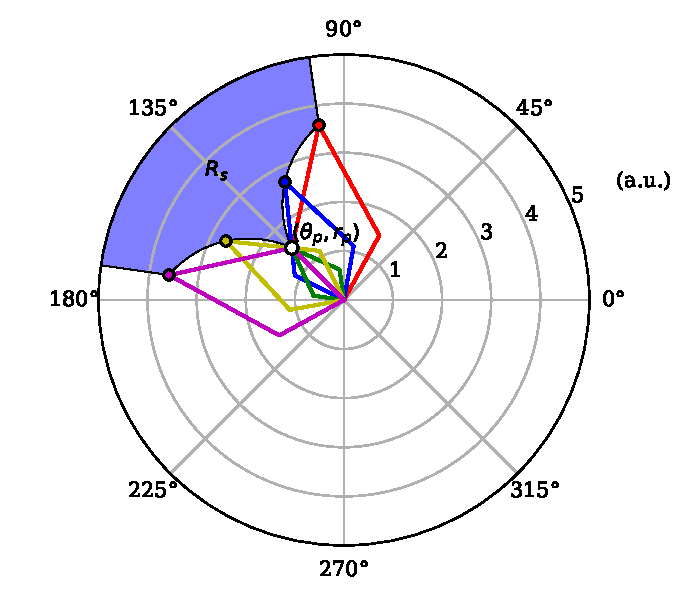
\includegraphics[width=4.5in]{shade_area}
	\captionof{figure}{Outlines of minimum-length fronds for a variety of angles to occupy the point $(\theta,s)=(3\pi/4,3/2)$.}
	\label{fig:shade_area}
\end{figure}

\subsection{Probability of Occupancy}
We are interested in the probability that, given a fixed point $(\theta,s)$, values of $l$ and $\theta_f$ chosen from the distributions described in Section \ref{sec:dist} will fall in the occupancy region.
This is found by integrating $P_{2D}(\theta_f, l)$ from \eqref{eqn:p2d} over $R_s(\theta,s)$, the occupancy region for the point of interest.

\begin{figure}[h]
	\centering
	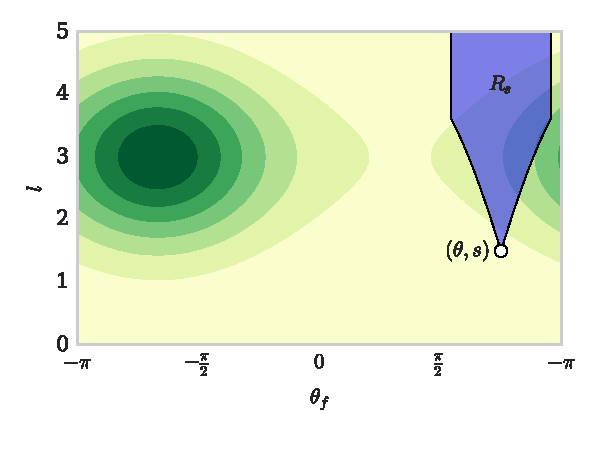
\includegraphics[width=4.5in]{cart_shade}
	\captionof{figure}{Contour plot of $P_{2D}(\theta_f,l)$ overlayed with the
    region in the $\theta_f$\nobreak--\nobreak$l$ plane which results in a frond occupying the point $(\theta,s)=(3\pi/4,3/2)$.}
	\label{fig:cart_shade}
\end{figure}

Integrating $P_{2D}(\theta_f,l)$ over $R_s(\theta,s)$ as depicted in Figure \ref{fig:cart_shade} yields the proportion of the population in the depth layer occupying the point $(\theta,s)$,
\begin{align}
		\tilde{P}_k(\theta,s,z)	&= \iint_{R_s(\theta,s)}
								P_{2D}(\theta_f,l)
								\,dl\,d\theta_f \nonumber \\
							&= \int_{\theta-\alpha}^{\theta+\alpha}
								\int_{l_{\min}(\theta_f)}^\infty
								P_{2D}(\theta_f,l)
								\,dl\,d\theta_f.
                \label{eqn:integrate_p2d}
\end{align}

Assuming that the depth layer has thickness $dz$ and contains $n_f$ fronds of thickness $f_t$,
the proportion of the vertical length of the discrete depth layer occupied by kelp at any position $(x,y,z)$ is given by
\begin{equation}
  P_k(x, y) = \frac{n_ff_t}{dz}\tilde{P}_k(x, y).
  \label{eqn:kelp_pk}
\end{equation}
In the continuum limit as the number of discrete depth depth layers approaches infinity, $P_k(x,y,z)$ can be interpreted as the probability of the point $(x,y,z)$ being occupied by kelp.
In a three dimensional context, the number of fronds is more likely to be specified by a number density $\rho_f=n_f/dz$ over the vertical length of the rope with units \SI{}{\per\m}, in which case
\begin{equation}
  P_k(x, y, z) = f_t \rho_f(z) \tilde{P}_k(x, y, z).
\end{equation}
Then, since the point $\vec{x}$ has a probability $P_k(\vec{x})$ of being occupied by kelp and a probability $(1-P_k(\vec{x}))$ of being occupied by the surrounding aquatic medium,
the effective absorption coefficient can be calculated as
\begin{equation*}
  \label{eqn:abs_field}
  a(\vec{x}) = P_k(\vec{x})a_k + (1-P_k(\vec{x}))a_w,
\end{equation*}
where $a_k$ is the absorption coefficient of the kelp alone, and $a_w$ is the absorption coefficient of the water and its dissolved and suspended contents.

\begin{figure}[h]
	\centering
	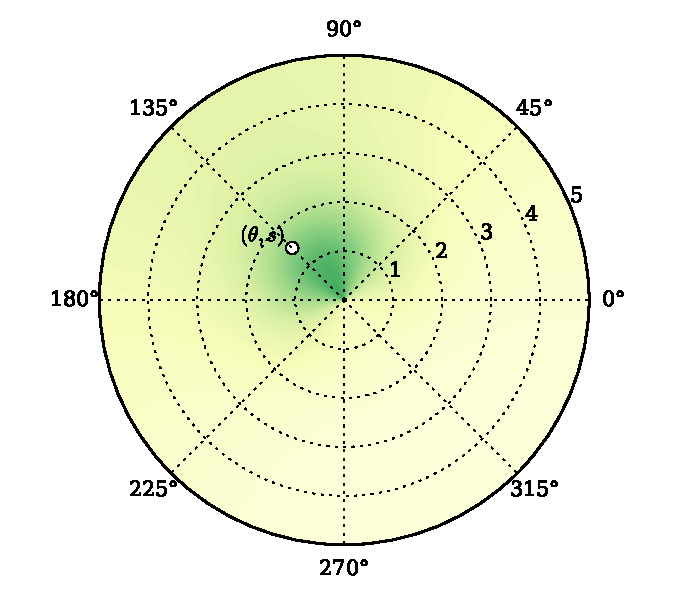
\includegraphics[width=4.5in]{prob_shade}
	\captionof{figure}{Contour plot of the probability of frond occupation sampled at 121 points using $\theta_f=2\pi/3,\eta v_w=1$.}
	\label{fig:prob_shade}
\end{figure}

\section{Discontinuity at the rope}
While the above model of the kelp distribution is straightforward to evaluate, it does have a significant numerical difficulty in its application.
Since the length and orientations are both continuous in the polar coordinates $s>0$ and $\theta$, the resulting kelp density and effective absorption coefficient are as well.
However, they are not necessarily continuous in Cartesian coordinates.
In the case of no water current, $v_w=0$, the flat von Mises distribution produces a continuous solution at the origin.
In the more general case, though, there is a high kelp density on one side of the origin in the direction of the current, and a low kelp density immediately on the other side.
Since the rope is assumed to be infinitely thin and have a fixed position, the sharp corners of the kelp fronds emanate from exactly the same point.
Hence, there is in general a discontinuity in the kelp distribution at the origin, and therefore its derivatives are unbounded on the domain.

This is not appealing numerically since the algorithms used in this thesis to solve the differential equation describing the light field are based on interpolation on a discrete Cartesian grid.
According to Taylor's theorem, the error incurred by performing such interpolation is bounded by a constant multiple of the appropriate maximum derivative of the interpolated function over the domain.
If the derivatives of the absorption coefficient are unbounded, then so too is the discretization error in the final solution.
That is, the solution is not guaranteed to converge.

Luckily, there is a straightforward solution, which is to post-process the spatial kelp distribution with a Gaussian blur in the $x$ and $y$ dimensions.
This is achieved via convolution of the solution with a 2D Gaussian kernel centered at the origin.
Any blur whatsoever is sufficient to bound the derivatives, and the larger the blur radius, the smaller they become.
Obviously, as the blur radius is increased, the kelp distribution tends toward a constant and no longer captures any information about the $xy$ distribution of the kelp.
Therefore, a small blur radius should be used.

\subsection{One dimensional Gaussian blur}
As a one dimensional analogy, consider the Heaviside step function,
\begin{equation*}
  H(x) = \begin{cases}
    0, & x < 0, \\
    1, & x > 0.
  \end{cases}
\end{equation*}
Clearly, the function is infinitely steep at the origin.
Consider the normalized Gaussian kernel centered at the origin with radius $\sigma_b$, given by
\begin{equation}
  k(x;\sigma_b) = \frac{1}{\sqrt{2\pi\sigma_b^2}} \exp\left({-\frac{x^2}{2\sigma_b^2}}\right).
\end{equation}
A blur is applied by convolving the function with the kernel according to the formula
\begin{align*}
  \tilde{H}(x) &= (k*H)(x) = \int_{-\infty}^{\infty}H(\tau)k(x-\tau;\sigma_b)\, d\tau \\
  &= \int_{0}^{\infty}k(x-\tau;\sigma_b)\, d\tau.
\end{align*}
The substitution $u=\tau=x,\, du=d\tau$ yields
\begin{equation*}
  \tilde{H}(x) = \int_{-x}^\infty k(u;\sigma_b)\, du.
\end{equation*}
Note that since the kernel is normalized, the integral from 0 to infinity is $1/2$.
Further, since the kernel is even, the integral over $[-x, 0]$ is equal to the integral over $[0, x]$.
Hence,
\begin{equation*}
  \tilde{H}(x) = \frac{1}{2} + \int_{0}^x k(u;\sigma_b)\, du.
\end{equation*}
Then, by the fundamental theorem of calculus, the derivative of the convolved function is simply $k(x;\sigma_b)$, whose maximum value is $k(0;\sigma_b) = 1/\sqrt{2\pi\sigma_b^2}$.
Then, since the derivative is a linear operator, this result can be generalized to the following statement:
Applying a Gaussian blur of radius $\sigma_b$ to a function with a maximum discontinuity of size $J$ produces a function whose first derivative is bounded by
\begin{equation*}
  \frac{1}{\sqrt{2\pi}}\frac{J}{\sigma_b}.
\end{equation*}
The same logic applies to directional derivatives of multidimensional scalar functions.

\subsection{Multidimensional Gaussian Blur}
\label{sec:gaussian_blur}
In light of the above arguments, the derivatives of the absorption coefficient are bounded by applying a Gaussian blur to $P_k$ before the calculation of $a(\vec{x})$.
This is done by convolving slices of $P_k$ in the $xy$--plane with the two--dimensional normalized Gaussian kernel
\begin{equation}
  \label{eqn:gaussian_kernel}
  K(x, y; \sigma_b) = \frac{1}{\sqrt{2\pi\sigma_b^2}} \exp\left(\frac{x^2 + y^2}{2\sigma_b^2}\right).
\end{equation}
Hence, the blurred solution is 
\begin{equation}
  \label{eqn:gaussian_blur}
  P_k^b(x, y, z) = \int_{-\infty}^\infty \int_{-\infty}^\infty K(x', y', z; \sigma_b) P_k(x-x', y-y', z)\, dx'\, dy'.
\end{equation}

A physical interpretation of this Gaussian blurring is that $P_k^b$ is the time--averaged kelp distribution, assuming that the rope is allowed to move horizontally, and $k(x, y; \sigma)$ is the PDF of the rope's location distribution.
This interpretation is a bit incongruous with the rest of the model since there is no other explicit mention of time--averaging; while the frond length and position distributions can be thought of as continuous approximations to the population distribution at a single point in time, this idea does not apply to the rope's position, since there is only one rope.

\subsection{Absorption coefficient plots}
% TODO: Clean up figures
A variety of numerically calculated absorption coefficient fields are shown here in order to demonstrate some key features of the kelp distribution.
In each figure, the absorption coefficient is plotted on the color axis, while the norm of its gradient is shown with contours, with brighter contour lines representing regions of large derivatives.
As mentioned above, large derivatives generate large discretization error, and are therefore undesirable.
Of course, the distributions must be sufficiently well--defined to capture the characteristics of the kelp.

Figure \ref{fig:kelp_dist_sharp} shows a sharp kelp distribution with an unrealistically high current velocity, with all fronds identically equal in length, and with no blurring applied.
Note the kite--shaped distribution, as expected.
Also note the regions of high derivatives near the origin and inner edges.
This sharp distribution requires excessively large numerical grids to approximate well, and is therefore undesirable.
\begin{figure}[H]
  \centering
  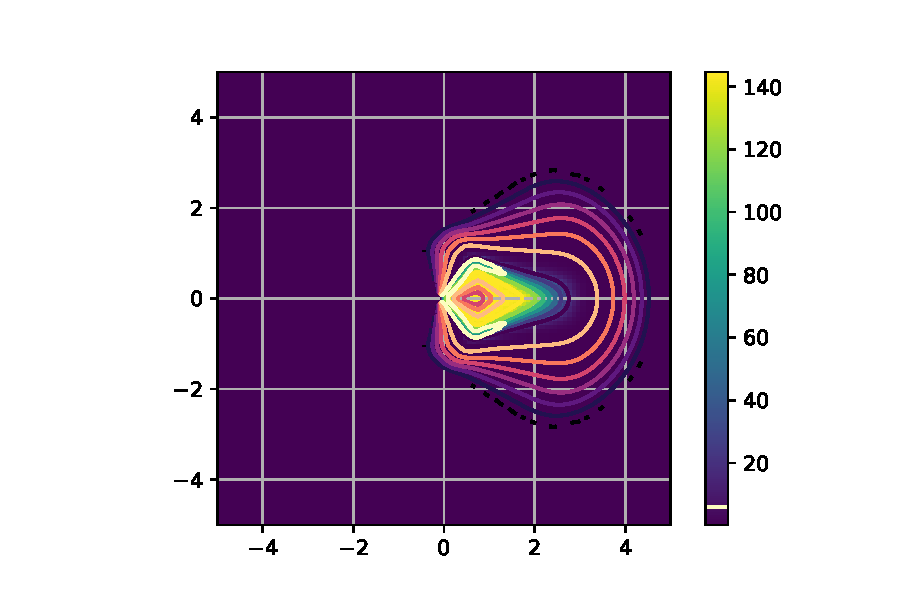
\includegraphics[width=5in]{kelp_dist_sharp}
  \caption{Absorption coefficient profile in the limiting case of $v_w>>1$, $\sigma_l=0$ and $\sigma_b=0$ demonstrates the kite--shaped fronds. Note the high gradient near the inner edge of the frond.}
  \label{fig:kelp_dist_sharp}
\end{figure}

In Figure \ref{fig:kelp_dist_smooth}, the current velocity has been reduced, and a nonzero standard deviation has been given to the frond distribution.
With a variety of frond lengths, the edges are no longer as clearly defined, although the general character of the distribution is sensible --- the kelp is most dense near the rope in the direction of the current.
However, note that there remains a small neighborhood of sharp derivatives encompassing the origin.
Such a distribution would still cause numerical difficulties for the numerical algorithm.

\begin{figure}[H]
  \centering
  \vspace{-3em}
  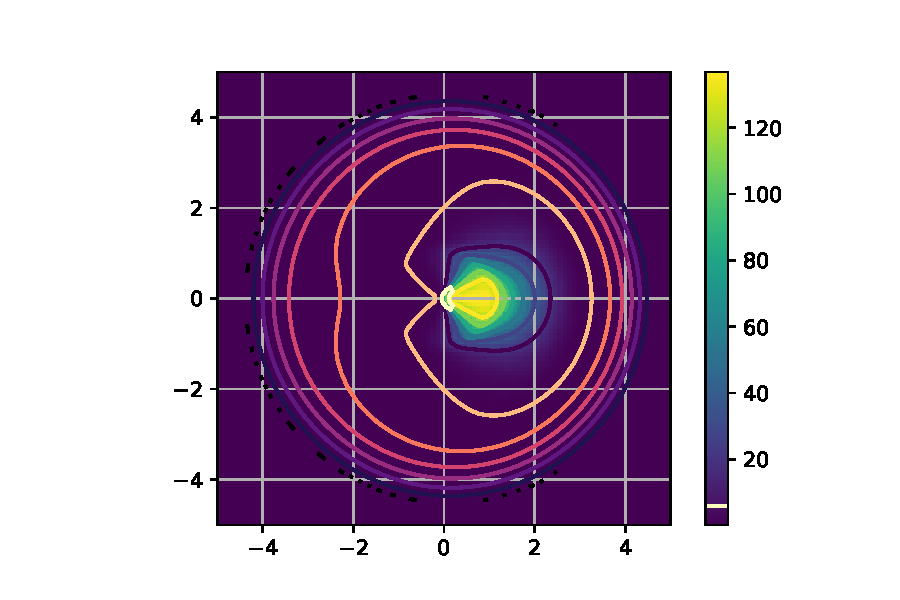
\includegraphics[width=5in]{kelp_dist_smooth}
  \caption{Absorption coefficient profile for realistic values of $v_w$ and $\sigma_l$, but with $\sigma_b=0$. Note the large gradient at the origin. By continuing to increase the plotting resolution, the gradient would be found to be unbounded.}
  \label{fig:kelp_dist_smooth}
\end{figure}

Figure \ref{fig:kelp_dist_smooth_smallblur} is similar to Figure \ref{fig:kelp_dist_smooth}, except it has been post--processed with a small Gaussian blur of radius \SI{10}{cm}, not so large that it significantly distorts the shape of the distribution, but sufficient to remove the discontinuity in the origin.
Such a kelp distribution is ideal, as it balances accuracy with ease of numerical approximation.
\begin{figure}[H]
  \centering
  \vspace{-3em}
  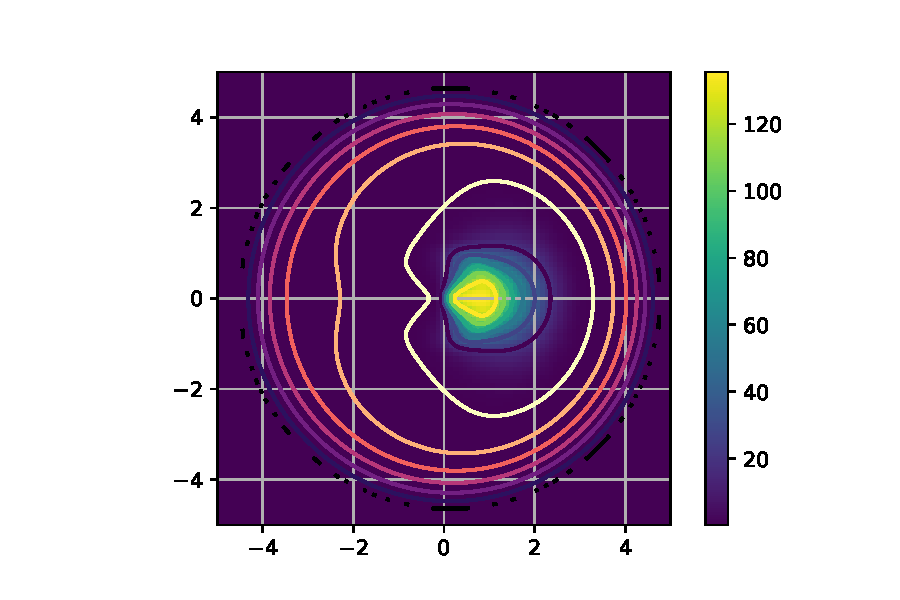
\includegraphics[width=5in]{kelp_dist_smooth_smallblur}
  \caption{A small blur radius of $\sigma_b=\SI{0.1}{\m}$ eliminates the derivative singularity at the origin.}
  \label{fig:kelp_dist_smooth_smallblur}
\end{figure}

In Figure \ref{fig:kelp_dist_smooth_blur}, too large of a blur has been applied; the character of the Gaussian kernel has overwhelmed that of the kelp distribution.
While this may still provide a better spatial description of the kelp than a fully horizontally uniform distribution, and unnecessary amount of information has been sacrificed for marginal gains in smoothness over Figure \ref{fig:kelp_dist_smooth_smallblur}.
Such a large blur is unlikely to reduce the discretization error, since other factors are contributing to it more significantly.
\begin{figure}[H]
  \centering
  \vspace{-3em}
  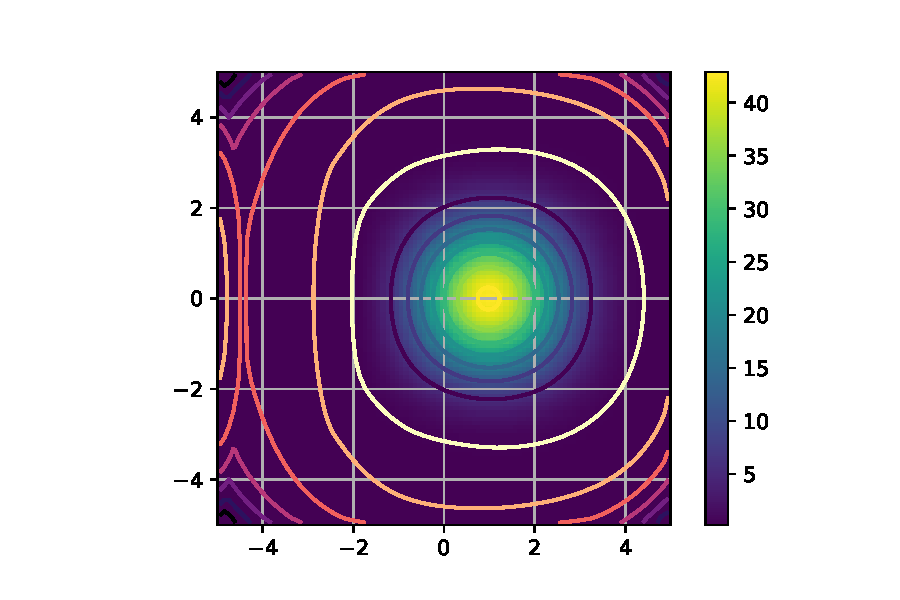
\includegraphics[width=5in]{kelp_dist_smooth_blur}
  \caption{Over-blurring kelp distribution with $\sigma_b=\SI{10}{\m}$ causes it to lose a great deal of spatial resolution. This should be avoided.}
  \label{fig:kelp_dist_smooth_blur}
\end{figure}

\chapter{LIGHT MODEL}
\label{chap:light}

Now that we have formulated the distribution of kelp throughout the medium, we introduce the Radiative Transfer Equation, which is used to calculate the light field.

\section{Optical Definitions}

\subsection{Radiometric Quantities}

One of the most fundamental quantities in optics is radiant flux $\Phi$, which is the has units of energy per time.
The quantity of primary interest in modeling the light field is radiance $L$, which is defined as the radiant flux per steradian per projected surface area perpendicular to the direction of propagation of the beam.
That is,

\begin{equation*}
	L = \frac{d^2\Phi}{dA d\omega}
\end{equation*}

Once the radiance $L$ is calculated everywhere, the irradiance is
\begin{equation*}
  I(\vec{x}) = \int_{4\pi}L(\vec{x},\vec{\omega})\, d\omega.
\end{equation*}
Integrating $I(\vec{x})$, which has units \SI{}{\W/m^2}, over the surface of a frond, produces the power (with units \SI{}{\W}) transmitted to the frond.
For details, see Section \ref{sec:perceived_irrad}.

Irradiance is sometimes given in units of moles of photons (a mole of photons is also called an Einstein) per second, with the conversion \cite{mobley_light_1994} given by
\begin{equation*}
  \SI{1}{\W\per\m^2} = \SI{4.2}{\micro\mole \,photons\per\second}.
\end{equation*}

\subsection{Inherent Optical Properties}
% TODO: Edit
We must now define a few inherent optical properties (IOPs) which depend only on the medium of propagation.
These phenomena are governed by three inherent optical properties (IOPs) of the
medium.
The absorption coefficient $a(\vec{x})$ (units m$^{-1}$) defines the
proportional loss of radiance per unit length.
The scattering coefficient $b$ (units m$^{-1}$), defines the proportional loss
of radiance per unit length, and is assumed to be constant over space.

The volume scattering function (VSF) $\beta(\Delta): [-1, 1] \to \RR^+$ (units sr$^{-1}$) defines the probability of light scattering at any given angle from its source.
Formally, given two directions $\vec{\omega}$ and $\vec{\omega}'$, $\beta(\vec{\omega} \cdot \vec{\omega}')$ is the probability density of light scattering from $\vec{\omega}$ into $\vec{\omega}'$ (or vice-versa).
Of course, since a single direction subtends no solid angle, the probability of scattering occurring exactly from $\vec{\omega}$ to $\vec{\omega}'$ is 0.
Rather, we say that the probability of radiance being scattered from a direction $\omega$ into an element of solid angle $\Omega$ is $\int_\Omega \beta(\vec{\omega} \cdot \vec{\omega}')\, d\vec{\omega}'$.

The VSF is normalized such that
\begin{equation*}
  \int_{-1}^1\beta(\Delta)\, d\Delta=\frac{1}{2\pi},
\end{equation*}
so that for any $\omega$,
\begin{equation*}
  \int_{4\pi}\beta(\vec{\omega}\cdot\vec{\omega}')\, d\vec{\omega}' = 1.
\end{equation*}
i.e., the probability of light being scattered to some direction on the unit sphere is 1.


\section{The Radiative Transfer Equation}
% TODO: Blurb
We now present the Radiative Transfer Equation, whose solution is the radiance in the medium as a function of position and angle.

\subsection{Ray Notation}
Consider a fixed position $\vec{x}$ and direction $\vec{\omega}$ such that
$\vec{\omega} \cdot \hat{z} \neq 0$.
% TODO: Just call $\vec{x_0}$ a point, not a function. Call it the projection to the surface.
Let $\vec{l}(\vec{x}, \vec{\omega}, s)$ denote the linear path containing $\vec{x}$ in the direction $\vec{\omega}$.
Assume that the ray is not horizontal.
Then, it originates either at the surface or bottom of the domain, with initial z coordinate given by
\begin{equation*}
  z_0 =
   \begin{cases}
    0, & \vec{\omega} \cdot \hat{z} < 0 \\
    \zmax, & \vec{\omega} \cdot \hat{z} > 0.
  \end{cases}
\end{equation*}
Hence, the ray path is parameterized as
\begin{equation}
  \vec{l}(\vec{x}, \vec{\omega}, s) = \frac{1}{\tilde{s}} (s\vec{x} + (\tilde{s} - s)\vec{x_0}(\vec{x}, \vec{\omega})),
  \label{eqn:ray_path}
\end{equation}
where
\begin{equation*}
  \vec{x_0}(\vec{x}, \vec{\omega}) = \vec{x} - \tilde{s} \vec{\omega}
\end{equation*}
is the origin of the ray, and 
\begin{equation*}
  \tilde{s} = \frac{\vec{x} \cdot \hat{z} - z_0}{\vec{\omega} \cdot \hat{z}}
\end{equation*}
is the path length from $\vec{x_0}(\vec{x}, \vec{\omega})$ to $\vec{x}$.

\subsection{Colloquial Description}
Denote the radiance at $\vec{x}$ in the direction $\vec{\omega}$ by $L(\vec{x}, \vec{\omega})$.
As light travels along $\vec{l}(\vec{x}, \vec{\omega}, s)$, interaction with the
medium produces three phenomena of interest:
\begin{enumerate}
  \item Radiance is decreased due to absorption.
  \item Radiance is decreased due to scattering out of the path to other
    directions.
  \item Radiance is increased due to scattering into the path from other
      directions.
\end{enumerate}

\subsection{Equation of Transfer}
Combining these phenomena yields the Radiative Transfer Equation along
$\vec{l}(\vec{x}, \vec{\omega})$,
\begin{equation}
  \label{eqn:rte1d}
  \frac{dL}{ds}(\vec{l}(\vec{x}, \vec{\omega}, s), \vec{\omega})
  = -(a(\vec{x}) + b)L(\vec{x}, \vec{\omega})
  + b \int_{4\pi} \beta(\vec{\omega}\cdot\vec{\omega}') L(\vec{x})\, d\omega',
\end{equation}
where $\int_{4\pi}$ denotes integration over the unit sphere.
The derivative of $L$ over the path can be rewritten as
\begin{align*}
  \frac{dL}{ds}(\vec{l}(\vec{x}, \vec{\omega}, s), \vec{\omega})
    &= \frac{d\vec{l}}{ds}(\vec{x}, \vec{\omega}, s) \cdot \nabla L(\vec{x}, \vec{\omega}', \vec{\omega}) \\
    &= \vec{\omega} \cdot \nabla L(\vec{x}, \vec{\omega}),
\end{align*}
which unveils the general form of the Radiative Transfer Equation,
\begin{equation*}
  \vec{\omega} \cdot \nabla L(\vec{x}, \vec{\omega})
  = -(a(\vec{x}) + b)L(\vec{x}, \vec{\omega})
  + b \int_{4\pi} \beta(\vec{\omega}\cdot\vec{\omega}') L(\vec{x}, \vec{\omega}')\, d\omega'
\end{equation*}

or, equivalently,
\begin{equation}
  \vec{\omega} \cdot \nabla L(\vec{x}, \vec{\omega})
  + a(\vec{x})L(\vec{x}, \vec{\omega})
  = b \left(
    \int_{4\pi} \beta(\vec{\omega}\cdot\vec{\omega}') L(\vec{x}, \vec{\omega}')\, d\omega'
    - L(\vec{x}, \vec{\omega})
  \right).
  \label{eqn:rte}
\end{equation}

\subsection{Boundary Conditions}

We use periodic boundary conditions in the $x$ and $y$ directions,
\begin{align*}
  L\left((\xmin, y, z), \vec{\omega}\right) &= L\left((\xmax, y, z), \vec{\omega}\right), \\
  L\left((x, \ymin, z), \vec{\omega}\right) &= L\left((x, \ymax, z), \vec{\omega}\right).
\end{align*}
In the $z$ direction, we specify a spatially uniform downwelling light just
under the surface of the water by a function $f(\vec{\omega})$.
Or if $\zmin>0$, then the radiance at $z=\zmin$ should be specified instead (as opposed to the radiance at the first grid cell center).
Further, we assume that no upwelling light enters the domain from the bottom, so
\begin{align*}
  L(\vec{x_s}, \vec{\omega}) &= f(\omega) \mbox{ if } \vec{\omega} \cdot \hat{z} > 0, \\ 
  L(\vec{x_b}, \vec{\omega}) &= 0 \mbox { if } \vec{\omega} \cdot \hat{z} < 0.
\end{align*}
 
\section{Low-Scattering Approximation}
In clear waters where absorption is more important than scattering, an asymptotic expansion can be used whereby the light field is generated through a sequence of discrete scattering events.
\subsection{Asymptotic Expansion}
Taking $b$ to be small, we introduce the asymptotic series
\newcommand{\Lasym}{L_0(\vec{x},\vec{\omega}) + b L_1(\vec{x},\vec{\omega}) + b^2 L_2(\vec{x},\vec{\omega}) + \cdots}
\newcommand{\Lasyms}{L_0(\vec{x_s},\vec{\omega}) + b L_1(\vec{x_s},\vec{\omega}) + b^2 L_2(\vec{x_s},\vec{\omega}) + \cdots}
\newcommand{\Lasymp}{L_0(\vec{x},\vec{\omega}') + b L_1(\vec{x},\vec{\omega}') + b^2 L_2(\vec{x},\vec{\omega}') + \cdots}
\begin{align*}
  L(\vec{x},\vec{\omega}) = \Lasym.
\end{align*}
Substituting the above into \eqref{eqn:rte} yields
\begin{align*}
    &\vec{\omega} \cdot \nabla \left[ \Lasym \right] \\
    &+ a(\vec{x}) \left[ \Lasym \right] \\
    &= b\Bigg(
      \int_{4\pi} \beta(\vec{\omega}\cdot\vec{\omega}')
      \left[ \Lasymp \right] \, d\vec{\omega}' \\
    &- \left[ \Lasym \right]
    \Bigg).
\end{align*}
Grouping like powers of $b$, we have the decoupled set of equations
\begin{align}
  \vec{\omega} \cdot \nabla L_0(\vec{x}, \vec{\omega}) + a(\vec{x})L_0(\vec{x}) &= 0,
  \label{eqn:asymptotics_0}\\
  \vec{\omega} \cdot \nabla L_1(\vec{x}, \vec{\omega}) + a(\vec{x})L_1(\vec{x})
  &= \int_{4\pi} \beta(\vec{\omega}\cdot\vec{\omega}') L_0(\vec{x}, \vec{\omega}')\,d\vec{\omega}' - L_0(\vec{x}, \vec{\omega}), \nonumber\\ 
  \vec{\omega} \cdot \nabla L_2(\vec{x}, \vec{\omega}) + a(\vec{x})L_2(\vec{x})
  &= \int_{4\pi} \beta(\vec{\omega}\cdot\vec{\omega}') L_1(\vec{x}, \vec{\omega}')\,d\vec{\omega}' - L_1(\vec{x}, \vec{\omega}). \nonumber \\ 
  &\vdots \nonumber
\end{align}
In general, for $n \geq 1$,
\begin{equation}
  \vec{\omega} \cdot \nabla L_n(\vec{x}, \vec{\omega}) + a(\vec{x})L_n(\vec{x})
  = \int_{4\pi} \beta(\vec{\omega}\cdot\vec{\omega}') L_{n-1}(\vec{x}, \vec{\omega}')\,d\vec{\omega}' - L_{n-1}(\vec{x}, \vec{\omega}).
  \label{eqn:asymptotics_n}
\end{equation}

For boundary conditions, let $\vec{x_s}$ be a point on the surface of the domain.
Then, 
\begin{equation*}
  \Lasyms =
  \begin{cases}
    f(\omega), & \hat{z}\cdot\omega > 0 \\
    0, & \mbox{otherwise},
  \end{cases}
\end{equation*}
which can be decomposed as
\begin{align}
  L_0(\vec{x}, \vec{\omega}) &=
  \begin{cases}
    f(\omega), & \hat{z}\cdot\omega > 0, \\
    0, & \mbox{otherwise},
  \end{cases}
  \label{eqn:asymptotics_bc_0} \\
  L_1(\vec{x}, \vec{\omega}) &= 0 \nonumber \\
  L_2(\vec{x}, \vec{\omega}) &= 0. \nonumber \\
  &\vdots \nonumber
\end{align}
In general, for $n \geq 1$,
\begin{equation}
  L_n(\vec{x}, \vec{\omega}) = 0.
  \label{eqn:asymptotics_bc_n}
\end{equation}

 
\subsection{Analytical Solution}
\label{sec:asymptotic_sol}

For all $\vec{x}, \vec{\omega}$, we consider the path $l(\vec{x}, \vec{\omega}, s)$ from \eqref{eqn:ray_path}.
We extract the absorption coefficient along the path,
\begin{equation*}
  \tilde{a}(s) = a(\vec{l}(\vec{x}, \vec{\omega}), s).
\end{equation*}
Then, the first equation from the asymptotic expansion, \eqref{eqn:asymptotics_0} and its associated boundary condition, \eqref{eqn:asymptotics_bc_0}, can be rewritten as
\begin{equation*}
  \left\{
  \begin{aligned}
  0 &= \frac{du_0}{ds}(s) + \tilde{a}(s) u_0(s) \\
  u_0(0) &= f(\vec{\omega}),
  \end{aligned}
  \right.
\end{equation*}
which we can solve by multiplying by the appropriate integrating factor, as follows.
\begin{align*}
  0 &= \exp\left(\int_0^s \tilde{a}(s')\, ds'\right) \frac{du_0}{ds} + \exp\left(\int_0^s \tilde{a}(s')\, ds'\right) \tilde{a}(s) u_0(s) \\
  &= \frac{d}{ds}\left[\exp\left(\int_0^s \tilde{a}(s')\, ds'\right) u_0(s)\right].
\end{align*}
Then, integrating both sides yields
\begin{align*}
  0 &= \int_0^s \frac{d}{ds'}\left[\exp\left(\int_0^{s'} \tilde{a}(s'')\, ds''\right) u_0(s')\right]\, ds' \\
  &= \exp\left(\int_0^s \tilde{a}(s')\, ds'\right) u_0(s) - f(\vec{\omega}).
\end{align*}
Hence,
\begin{equation}
  u_0(s) = f(\omega) \exp\left(-\int_0^s \tilde{a}(s)\, ds\right).
  \label{eqn:asymptotics_soln_0}
\end{equation}
Then, we convert back from path length $s$ to the spatial coordinate $\vec{x}$ using
\begin{equation*}
  L_0(\vec{l}(\vec{x}, \vec{\omega},s), \vec{\omega}) = u_0(s).
\end{equation*}

The $n \geq 1$ equations have a nonzero right-hand side, which we call the effective source, $g_n(s)$.
This can be similarly extracted along a ray path as
\begin{equation*}
  g_n(s) = \int_{4\pi} \beta(\vec{\omega}\cdot\vec{\omega}')
  L_{n-1}(\vec{l}(\vec{x}, \vec{\omega'}, s), \vec{\omega}')\,d\vec{\omega}' - L_{n-1}(\vec{l}(\vec{x}, \vec{\omega}, s), \vec{\omega}).
\end{equation*}
Then, since $g_n$ depends only on $L_{n-1}$, it is independent of $u_n$, which allows \eqref{eqn:asymptotics_n} and its boundary condition, \eqref{eqn:asymptotics_bc_n}, to be written as the first order, linear ordinary differential equation along the ray path,
\begin{equation*}
  \left\{
  \begin{aligned}
    g_n(s) &= \frac{du_n}{ds}(s) + \tilde{a}(s)u_n(s) \\
    u_n(0) &= 0
  \end{aligned}
  \right.
\end{equation*}
As with the $n=0$ equation, the solution is found by multiplying by the appropriate integrating factor.
\begin{align*}
  \exp\left(\int_0^s \tilde{a}(s')\, ds'\right) g_n(s) &= \exp\left(\int_0^s \tilde{a}(s')\, ds'\right) \frac{du_n}{ds} + \exp\left(\int_0^s \tilde{a}(s')\, ds'\right) \tilde{a}(s) u_n(s) \\
  &= \frac{d}{ds}\left[\exp\left(\int_0^s \tilde{a}(s')\, ds'\right) u_n(s)\right].
\end{align*}
Integrating both sides yields
\begin{align*}
  \int_0^s\exp\left(\int_0^{s'} \tilde{a}(s'')\, ds''\right) g_n(s')\, ds' &= \int_0^s \frac{d}{ds'}\left[\exp\left(\int_0^{s'} \tilde{a}(s'')\, ds''\right) u_n(s')\right]\, ds' \\
  &= \exp\left(\int_0^s \tilde{a}(s')\, ds'\right) u_n(s).
\end{align*}
Hence,
\begin{equation*}
  u_n(s) = \exp\left(-\int_0^s \tilde{a}(s')\, ds'\right) \int_0^s\exp\left(\int_0^{s'} \tilde{a}(s'')\, ds''\right) g_n(s')\, ds',
\end{equation*}
which simplifies to
\begin{equation}
  u_n(s) = \int_0^sg_n(s')\exp\left( -\int_{s''}^{s'}\tilde{a}(s'')\,ds'' \right)\, ds'.
  \label{eqn:asymptotics_soln_n}
\end{equation}
As before, the conversion back to spatial coordinates is
\begin{equation*}
  L_n(\vec{l}(\vec{x}, \vec{\omega}, s), \vec{\omega}) = u_n(s).
\end{equation*}

\chapter{NUMERICAL SOLUTION}
\label{chap:numerical}

In this chapter, the mathematical details involved in the numerical solution of the previously described equations are presented.
It is assumed that this model is run in conjunction with a model describing the growth of kelp over its life cycle, which calls this light model periodically to update the light field.

\section{Super-Individuals}

The algorithm described in this chapter has two components.
First, a probabilistic description of the kelp is generated at each point in a discrete spatial grid.
Second, optical properties of the resulting kelp-water medium are derived, and the light field is calculated.
The first component is described here.

\subsection{Frond Length Distribution}

Rather than model each kelp frond, a subset of the population, called super-individuals, are modelled explicitly, and are considered to represent many identical individuals, as in \citep{scheffer_super-individuals_1994}.
Specifically, at each depth $k$, there are $n$ super-individuals, indexed by $i$.
Super-individual $i$ has a frond area $A_{ki}$ and represents $n_{ki}$ individual fronds.

From \eqref{eqn:length-from-area}, the frond length of the super-individual is $l_{ki} = \sqrt{2A_{ki}f_r}$.
Given the super-individual data, we calculate the mean $\mu$ and standard deviation $\sigma$ frond
lengths using the formulas:
\begin{equation}
  \mu_k = \frac{\ds \sum_{i=1}^N l_{ki}}{\ds \sum_{i=1}^N n_{ki}},
\end{equation}
\begin{equation}
  \sigma_k = \frac{\ds \sum_{i=1}^N \left( l_{ki} - \mu_k \right)^2}{\ds \sum_{i=1}^N n_{ki}}.
\end{equation}
We then assume that frond lengths are normally distributed in each depth layer
with mean $\mu_k$ and standard deviation $\sigma_k$.

\section{Discrete Grid}
The following is a description of the uniform, rectangular spatial-angular grid used
in the numerical implementation of this model.
It is assumed that all simulated quantities are constant over the interior of a
grid cell.

The number of grid cells in each dimension are denoted by $n_x$, $n_y$, $n_z$,
$n_\theta$, and $n_\phi$, with uniform spacings $dx$, $dy$, $dz$, $d\theta$, and
$d\phi$ between adjacent grid points.

The following indices are assigned to each dimension:
\begin{align}
  x &\to i \\
  y &\to j \\
  z &\to k \\
  \theta &\to l \\
  \phi &\to m
\end{align}

It is convenient, however, to use a single index $p$ to refer to directions $\vec{\omega}$ rather than referring to $\theta$ and $\phi$ separately.
Then, the center of a generic grid cell will be denoted as
$(x_i, y_j, z_k, \vec{\omega}_p)$, and the boundaries between adjacent grid cells
will be referred to as \textit{edges}.
One-indexing is employed throughout this document.

\subsection{Spatial Grid}
\begin{figure}[H]
  \centering
  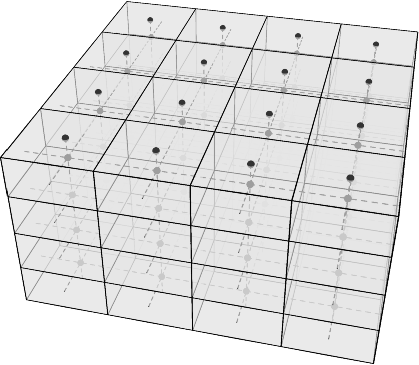
\includegraphics[width=8cm]{spatialgrid.pdf}
  \caption{Spatial grid}
  \label{fig:spatial_grid}
\end{figure}

\begin{align}
  dx &= \frac{x_{\max}-x_{\min}}{n_x} \\ 
  dy &= \frac{y_{\max}-y_{\min}}{n_y} \\ 
  dz &= \frac{z_{\max}-z_{\min}}{n_z}
\end{align}

Denote the edges as 
\begin{align}
  x_i^e &= (i-1)x \mbox{ for } i=1,\ldots,n_x \\
  y_j^e &= (j-1)y \mbox{ for } j=1,\ldots,n_y \\
  z_k^e &= (k-1)z \mbox{ for } k=1,\ldots,n_z 
\end{align}

and the cell centers as
\begin{align}
  x_i &= (i-1/2)dx \mbox{ for } i=1,\ldots,n_x \\
  y_j &= (j-1/2)dy \mbox{ for } j=1,\ldots,n_y \\
  z_k &= (k-1/2)dz \mbox{ for } k=1,\ldots,n_z
\end{align}

Note that in this convention, there are the same number of edges and cells,
and edges preceed centers.

% TODO: Not sure about this here.
Also, note that no grid center is located on the plane $z=0$.
The surface radiance boundary condition is treated separately.

\subsection{Angular Grid}
\begin{figure}[H]
  \centering
  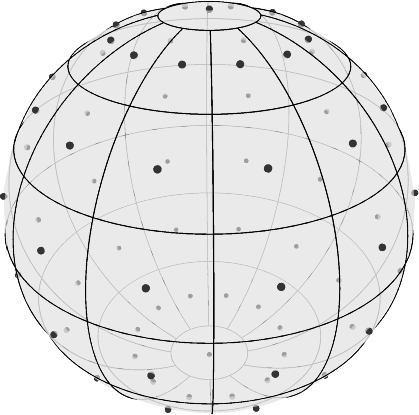
\includegraphics[width=8cm]{angulargrid.pdf}
  \caption{Angular grid at each point in space}
  \label{fig:angular_grid}
\end{figure}

Now, we define the azimuthal angle such that
\begin{align}
  \theta_l = (l-1)d\theta.
\end{align}
For the sake of periodicity, we need
\begin{align}
  \theta_1 &= 0, \\
  \theta_{n_\theta} &= 2\pi-d\theta,
\end{align}
which requires
\begin{equation}
  d\theta = \frac{2\pi}{n_\theta}.
\end{equation}

For the polar angle, we similarly let
\begin{equation}
  \phi_m = (m-1)d\phi
\end{equation}

Since the polar azimuthal is not periodic, we also store the endpoint, so
\begin{align}
  \phi_1 &= 0, \\
  \phi_{n_\phi} &= \pi.
\end{align}

This gives us
\begin{align}
  d\phi &= \frac{\pi}{n_\phi-1}.
\end{align}

It is also useful to define the edges between angular grid cells as
\begin{alignat}{3}
  \theta_l^e &= (l-1/2) d\theta, &\quad l&=1,\ldots,n_\theta \\
  \phi_m^e &= (m-1/2) d\phi, &\quad m&=1,\ldots,n_\phi-1.
\end{alignat}

Note that while $\theta$ has its final edge following its final center, this is
not the case for $\phi$.

\begin{figure}[h]
  \centering
  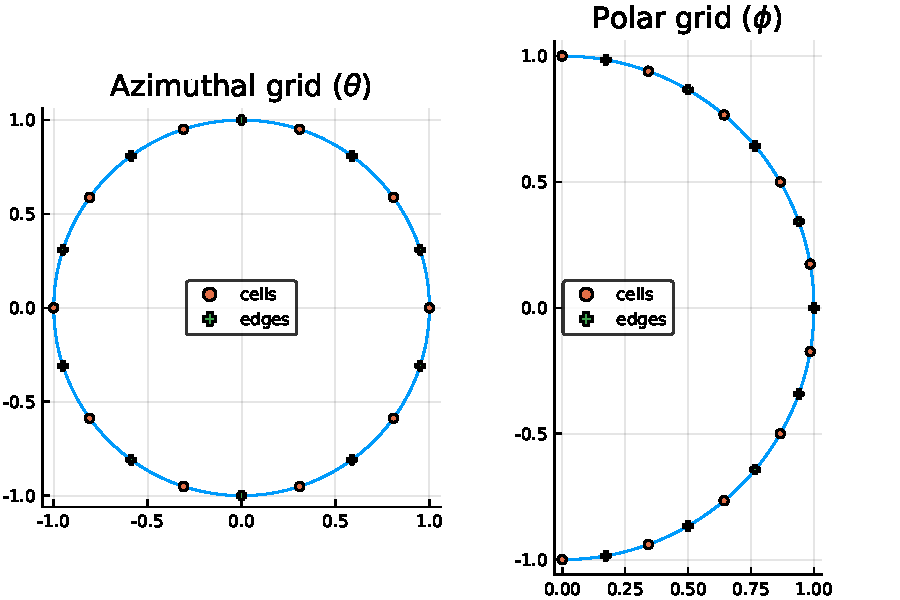
\includegraphics[width=.75\linewidth]{angular_grid_plots}
  \caption{Angular grid}
\end{figure}

As shown in Figure \ref{fig:angular_grid}, $\phi=0$ and $\phi=\pi$, called
the north ($+z$) and south ($-z$) poles respectively, are treated separately.
The total number of angles considered is $n_{\vec{\omega}} = n_\phi n_\theta -
2(n_\theta-1)$.
Since the poles create a non-rectangular angular grid in the sense that
$n_{\vec{\omega}}$ is not the product of two integers, it is advantageous to use
a single variable $p=1,\ldots,n_{\vec{\omega}}$ to index angles $\vec{\omega} =
(\theta, \phi)$ such that $p \in \left\{ 2,\ldots,n_{\vec{\omega}}-1 \right\}$ refers to the interior
of the angular grid, and $p=1$ and $p=n_{\vec{\omega}}$ refer to the
north and south poles respectively.
The following notation is used.
\begin{align}
  \hat{l}(p) &= \mbox{mod1}(p, n_\theta) \\
  \hat{m}(p) &= \ceil(p/n_\theta) + 1 \\
  \hat{\theta}_p &= \theta_{\hat{l}(p)} \\
  \hat{\phi}_p &= \phi_{\hat{m}(p)}
\end{align}

Thus, it follows that
\begin{equation}
  p = \left( \hat{m}(p)-2\right)n_\theta + \hat{l}(p).
\end{equation}

Accordingly, define
\begin{equation}
  \hat{p}(l,m) = (m-1)n_\theta + l.
\end{equation}

Further, we refer to the angular grid cell centered at $\vec{\omega}_p$ as $\Omega_p$, and the solid angle subtended by $\Omega_p$ is denoted $\abs{\Omega_p}$.
The areas of the grid cells are calculated as follows.
Note that there is a temporary abuse of notation in that the same symbols ($d\theta$ and $d\phi$) are being used for infinitessimal differential and for finite grid spacing.

For the poles, we have
\begin{align}
  \abs{\Omega_1} = \abs{\Omega_\nomega} &= \int_{\Omega_1} d{\vec{\omega}} \\
  &= \int_0^{2\pi}\int_0^{d\phi/2} \sin\phi\, d\phi\, d\theta \\
  &= 2\pi \cos\phi \Big|_{d\phi/2}^0 \\
  &= 2\pi(1-\cos(d\phi/2))
\end{align}

And for all other angular grid cells,
\begin{align}
  \abs{\Omega_p} &= \int_{\Omega_p} d{\vec{\omega}} \\
                 &= \int_{\theta_l^e}^{\theta_{l+1}^e}\int_{\phi_m^e}^{\phi_{m+1}^e} \sin(\phi)\, d\phi\, d\theta \\
                 &= d\theta \int_{\phi_m^e}^{\phi_{m+1}^e} \sin(\phi)\, d\phi \\
                 &= d\theta\left( \cos(\phi_m^e)-\cos(\phi_{m+1}^e) \right).
\end{align}


\subsection{Angular Quadrature}
We assume that all quantities are constant within a spatial-angular grid cell.
We therefore employ the midpoint rule for both spatial and angular integration.

Define the \textit{angular characteristic function}
\begin{equation}
  \mathcal{X}^\Omega_p(\vec{\omega}) = \begin{cases}
    1, & \vec{\omega} \in \Omega_p \\
    0, & \mbox{otherwise}
  \end{cases}
\end{equation}

\begin{align}
  \int_{4\pi} f(\vec{\omega})\, d\vec{\omega} &= \int_{4\pi} \sum_{p=1}^\nomega f_p \mathcal{X}^\Omega_p(\vec{\omega})\, d\vec{\omega} \\
  &= \sum_{p=1}^\nomega f_p \int_{4\pi} \mathcal{X}^\Omega_p(\vec{\omega})\, d\vec{\omega} \\
  &= \sum_{p=1}^\nomega f_p \int_{\Omega_p} d\vec{\omega} \\
  &= \sum_{p=1}^\nomega f_p \abs{\Omega_p}
\end{align}

 \subsection{Scattering Integral}

Specifically, we integrate $\beta$ to determine the amount of light scattered between angular grid cells.

Consider two angular grid cells, $\Omega$ and $\Omega'$.
The average probability density of scattering from $\vec{\omega} \in \Omega$ to $\vec{\omega}' \in \Omega'$ (or vice versa) is
\begin{equation}
  \beta_{pp'} = \frac{1}{\abs{\Omega}\abs{\Omega'}} \int_\Omega\int_{\Omega'}\beta(\vec{\omega}\cdot\vec{\omega}')\, d\vec{\omega'}\, d\vec{\omega}
\end{equation}

Denote the radiance at $(x_i, y_j, z_k, \vec{\omega}_p)$ by $L_{ijkp}$.
% TODO: Be more careful here.
Then, the total radiance scattered into $\Omega_p$ from $\Omega_{p'}$ is
\begin{align}
  \int_{\Omega}\int_{\Omega'}\beta(\vec{\omega} \cdot \vec{\omega}')L(\vec{x},\vec{\omega}')\, d\vec{\omega}'\, d\vec{\omega}
  &= L_{ijkp'} \int_\Omega\int_{\Omega_{p'}} \beta(\vec{\omega} \cdot \vec{\omega}')\, d\vec{\omega}'\, d\vec{\omega} \\
  &= \beta_{pp'}\abs{\Omega}\abs{\Omega'}L_{ijkp'}.
\end{align}
Hence, the average radiance scattered is $\beta_{pp'}\abs{\Omega'}L_{ijkp'}.$

\section{Finite Difference}

We now discuss the discretization of derivatives on the spatial grid.

\subsection{Discretization}

For the spatial interior of the domain, we use the 2nd order central difference formula (CD2) to approximate the derivatives, which is
\begin{equation}
    \tag{CD2}
    f'(x) = \frac{f(x+dx)-f(x-dx)}{2dx} + \mathcal{O}(dx^3).
\end{equation}

When applying the PDE on the upper or lower boundary, we use the forward and backward difference (FD2 and BD2) formulas respectively.
Omitting $\mathcal{O}(dx^3)$, we have
\begin{equation}
    \tag{FD2}
    \label{eq:FD2}
    f'(x) = \frac{-3f(x)+4f(x+dx)-f(x+2dx)}{2dx}
\end{equation}
\begin{equation}
    \tag{BD2}
    \label{eq:BD2}
    f'(x) = \frac{3f(x)-4f(x-dx)+f(x-2dx)}{2dx}
\end{equation}

For the upper and lower boundaries, we need an asymmetric finite difference
method.
In general, the Taylor Series of a function $f$ about $x$ is
\begin{equation}
  f'(x+\varepsilon) = \sum_{n=1}^\infty \frac{f^{(n)}(x)}{n!} \varepsilon^n \\
\end{equation}

Truncating after the first few terms, we have
\begin{equation}
  \label{eqn:afd1}
  f'(x+\varepsilon)  = f(x) + f'(x)\varepsilon + \frac{f''(x)}{2}\varepsilon^2 + \mathcal{O}(\varepsilon^3)
\end{equation}

Similarly, replacing $\varepsilon$ with $-\varepsilon/2$ we have
\begin{equation}
  \label{eqn:afd2}
  f'(x-\frac{\varepsilon}{2}) = f(x) - \frac{f'(x)\varepsilon}{2} + \frac{f''(x)\varepsilon^2}{8} + \mathcal{O}(\varepsilon^3).
\end{equation}

Rearranging \eqref{eqn:afd1} produces
\begin{equation}
  \label{eqn:afd3}
  f''(x)\varepsilon^2 = 2f(x+\varepsilon) - 2f(x) - 2f'(x)\varepsilon + \mathcal{O}(\varepsilon^3)
\end{equation}

Combining \eqref{eqn:afd2} with \eqref{eqn:afd3} gives
\begin{align*}
  \varepsilon f'(x) &= 2f(x) - 2f(x-\frac{\varepsilon}{2}) + f''(x)\frac{\varepsilon^2}{8} + \mathcal{O}(\varepsilon^3) \\
                    &= 2f(x) - 2f(x-\frac{\varepsilon}{2}) + \frac{f(x+\varepsilon)}{4} - \frac{f(x)}{4} - \frac{f'(x)\varepsilon}{4} + \mathcal{O}(\varepsilon^3) \\
                    &= \frac{4}{5}\left( 2f(x)-2f(x-\frac{\varepsilon}{2}) + \frac{f(x+\varepsilon)}{4} - \frac{f(x)}{4} \right) + \mathcal{O}(\varepsilon^3)
\end{align*}

Then, dividing by $\varepsilon$ gives
\begin{equation}
  f'(x) = \frac{-8f(x-\frac{\varepsilon}{2}) + 7f(x) + f(x+\varepsilon)}{5\varepsilon} + \mathcal{O}(\varepsilon^2)
\end{equation}

Similarly, substituting $\varepsilon \to -\varepsilon$, we have 
\begin{equation}
  f'(x) = \frac{- f(x-\varepsilon) - 7f(x) + 8f(x+\frac{\varepsilon}{2})}{5\varepsilon} + \mathcal{O}(\varepsilon^2)
\end{equation}


\subsection{Difference Equation}

%TODO: Periodic $x,y$

In general, we have

\begin{equation}
  \vec{\omega} \cdot \nabla L_p = -(a+b) L_p + \sum_{p'=1}^{n_{\vec{\omega}}} \beta_{pp'}L_{p'}.
\end{equation}

Then,
\begin{equation}
  \vec{\omega} \cdot \nabla L_p + (a+b(1-\beta_{pp'}))L_p - \sum_{p'=1}^{n_{\vec{\omega}}} \beta_{pp'} L_{p'} = 0
\end{equation}

Interior:
\begin{equation}
  \begin{aligned}
    0 &= \frac{L_{i+1,jkp}-L_{i-1,jkp}}{2dx}\sin\hat{\phi}_p\cos\hat{\theta}_p \\
    &+ \frac{L_{i,j+1,kp}-L_{i,j-1,kp}}{2dy}\sin\hat{\phi}_p\sin\hat{\theta}_p \\
    &+ \frac{L_{ij,k+1,p}-L_{ij,k-1,p}}{2dz}\cos\hat{\phi}_p \\
    &+ (a_{ijk}+b(1-\beta_{pp'}))L_{ijkp}  - \sum_{p'=1}^{n_{\vec{\omega}}} \beta_{pp'} L_{ijkp'}
  \end{aligned}
\end{equation}

Surface downwelling (BC):
\begin{equation*}
  \begin{aligned}
    0 &= \frac{L_{i+1,jkp}-L_{i-1,jkp}}{2dx}\sin\hat{\phi}_p\cos\hat{\theta}_p \\
    &+ \frac{L_{i,j+1,kp}-L_{i,j-1,kp}}{2dy}\sin\hat{\phi}_p\sin\hat{\theta}_p \\
    &+ \frac{-8f_p + 7L_{ijkp} + L_{ij,k+1,p}}{5dz}\cos\hat{\phi}_p \\
    &+ (a_{ijk}+b(1-\beta_{pp'}))L_{ijkp} \\
    &- \sum_{p'=1}^{n_{\vec{\omega}}} \beta_{pp'} L_{ijkp'}.
  \end{aligned}
\end{equation*}

Combining $L_{ijkp}$ terms on the left and moving the boundary condition to the
right gives

\begin{equation}
  \begin{aligned}
    &\frac{L_{i+1,jkp}-L_{i-1,jkp}}{2dx}\sin\hat{\phi}_p\cos\hat{\theta}_p \\
    + &\frac{L_{i,j+1,kp}-L_{i,j-1,kp}}{2dy}\sin\hat{\phi}_p\sin\hat{\theta}_p \\
    + &\frac{L_{ij,k+1,p}}{5dz}\cos\hat{\phi}_p \\
    + &(a_{ijk}+b(1-\beta_{pp'}) + \frac{7}{5dz} \cos\hat{\phi}_p)L_{ijkp} \\
    - &\sum_{p'=1}^{n_{\vec{\omega}}} \beta_{pp'} L_{ijkp'} = \frac{8f_p}{5dz} \cos\hat{\phi}_p.
  \end{aligned}
\end{equation}

Likewise for the bottom boundary condition, we have

\begin{equation}
  \begin{aligned}
    0 &= \frac{L_{i+1,jkp}-L_{i-1,jkp}}{2dx}\sin\hat{\phi}_p\cos\hat{\theta}_p \\
    &+ \frac{L_{i,j+1,kp}-L_{i,j-1,kp}}{2dy}\sin\hat{\phi}_p\sin\hat{\theta}_p \\
    &- \frac{L_{ij,k-1,p}}{5dz}\cos\hat{\phi}_p \\
    &+ (a_{ijk}+b(1-\beta_{pp'}) - \frac{7}{5dz}\cos\hat{\phi}_p)L_{ijkp} \\
    &- \sum_{p'=1}^{n_{\vec{\omega}}} \beta_{pp'} L_{ijkp'}.
  \end{aligned}
\end{equation}

Now, for upwelling light at the first depth layer (non-BC), we apply FD2.
\begin{equation}
  \begin{aligned}
    0 &= \frac{L_{i+1,jkp}-L_{i-1,jkp}}{2dx}\sin\hat{\phi}_p\cos\hat{\theta}_p \\
    &+ \frac{L_{i,j+1,kp}-L_{i,j-1,kp}}{2dy}\sin\hat{\phi}_p\sin\hat{\theta}_p \\
    &+ \frac{-3L_{ijkp} + 4L_{ij,k+1,p} - L_{ij,k+2,p}}{2dz}\cos\hat{\phi}_p \\
    &+ (a_{ijk}+b(1-\beta_{pp'}))L_{ijkp} \\
    &- \sum_{p'=1}^{n_{\vec{\omega}}} \beta_{pp'} L_{ijkp'}.
  \end{aligned}
\end{equation}

Grouping $L_{ijkp}$ terms gives
\begin{equation}
  \begin{aligned}
    0 &= \frac{L_{i+1,jkp}-L_{i-1,jkp}}{2dx}\sin\hat{\phi}_p\cos\hat{\theta}_p \\
    &+ \frac{L_{i,j+1,kp}-L_{i,j-1,kp}}{2dy}\sin\hat{\phi}_p\sin\hat{\theta}_p \\
    &+ \frac{4L_{ij,k+1,p} - L_{ij,k+2,p}}{2dz}\cos\hat{\phi}_p \\
    &+ \left(a_{ijk}+b(1-\beta_{pp'}) - 3\frac{\cos\hat\phi_p}{2dz} \right)L_{ijkp} \\
    &- \sum_{p'=1}^{n_{\vec{\omega}}} \beta_{pp'} L_{ijkp'}.
  \end{aligned}
\end{equation}

Similarly, for downwelling light at the lowest depth layer, we have
\begin{equation}
  \begin{aligned}
    0 &= \frac{L_{i+1,jkp}-L_{i-1,jkp}}{2dx}\sin\hat{\phi}_p\cos\hat{\theta}_p \\
    &+ \frac{L_{i,j+1,kp}-L_{i,j-1,kp}}{2dy}\sin\hat{\phi}_p\sin\hat{\theta}_p \\
    &+ \frac{-4L_{ij,k-1,p} + L_{ij,k-2,p}}{2dz}\cos\hat{\phi}_p \\
    &+ \left(a_{ijk}+b(1-\beta_{pp'}) + 3\frac{\cos\hat\phi_p}{2dz} \right)L_{ijkp} \\
    &- \sum_{p'=1}^{n_{\vec{\omega}}} \beta_{pp'} L_{ijkp'}
  \end{aligned}
\end{equation}

\subsection{Structure of Linear System}

%TODO: This
Describe layout of matrix.

\begin{table}[H]
  \centering
  \begin{tabular}{p{\linewidth/3}p{\linewidth/3}p{\linewidth/3}}
    \toprule
    \textbf{Derivative case} & \textbf{\# nonzero/row} & \textbf{\# of rows} \\
    \midrule
    interior & $\nomega+6$ & $n_xn_y(n_z-2)\nomega$ \\
    surface downwelling & $\nomega+5$ & $n_xn_y\nomega/2$ \\
    bottom upwelling & $\nomega+5$ & $n_xn_y\nomega/2$ \\
    surface upwelling & $\nomega+6$ & $n_xn_y\nomega/2$ \\
    bottom downwelling & $\nomega+6$ & $n_xn_y\nomega/2$ \\
  \end{tabular}
  \caption{Breakdown of nonzero matrix elements by derivative case}
\end{table}

Number of rows/columns: $n_xn_yn_zn_{\vec{\omega}}$

Number of nonzero RHS entries: $n_xn_yn_z/2$

Total number of nonzero matrix entries: $n_xn_yn_{\vec{\omega}} \left[n_z(n_{\vec{\omega}}+6)-1 \right]$

\subsection{GMRES}
% TODO: Fill this in
GMRES is a Krylov Subspace method. These work like this. Here's what's special
about GMRES. Advantages. Drawbacks. Not practical for running in SINMOD.

\section{Numerical Asymptotics}

Given a position $\vec{x}$ and direction $\vec{\omega}$, a path through the discrete grid can be constructed as described in Appendix \ref{chap:ray_tracing}, from which we can extract piecewise constant variations of the path absorption coefficient, $\tilde{a}(s)$ and the effective source, $g_n(s)$ from \ref{sec:asymptotic_sol}.
Then, we proceed as follows.

* Here are the equations for calculating the double integral over ray paths
required for the asymptotics. It will hopefully make more sense once I add words
to accompany the symbols.

Let
\begin{align}
  g_n(s) &= \sum_{i=1}^{N-1}g_{ni}\mathcal{X}_i(s) \\
  \tilde{a}(s) &= \sum_{i=1}^{N-1}\tilde{a}_{i}\mathcal{X}_i(s) \\
\end{align}

and
\begin{equation}
  \mathcal{X}_i(s) = \begin{cases}
    1, & a_I \leq s < s_{i+1} \\
    0, & \mbox{otherwise}
    \end{cases}
\end{equation}

and $\left\{s_i\right\}_{i=1}^N$ is increasing.

Let $ds_i = s_{i+1} - s_i$.

Let $\hat{i}(s) = \min\left\{ i \in \{1,\ldots,N\} : s_i>s \right\}$.
Let $\tilde{d}(s) = s_{\hat{i}(s)}-s$.

We have $s_1 = 0$ and $s_N = \tilde{s}$.


\begin{align}
  u_n(\tilde{s}) &= \int_0^{\tilde{s}}g_n(s')\exp\left( -\int_{s''}^{s'}\tilde{a}(s'')\,ds'' \right)\, ds' \\
  &= \int_0^{s_N} \sum_{i=1}^{N-1}g_{ni}\mathcal{X}_i(s') \exp\left( -\int_{s''}^{s'}\sum_{j=1}^{N-1}\tilde{a}_{j}\mathcal{X}_j(s'')\,ds'' \right)\, ds' \\
  &= \sum_{i=1}^{N-1}g_{ni}\int_0^{s_N} \mathcal{X}_i(s') \exp\left( -\sum_{j=1}^{N-1}\tilde{a}_{j}\int_{s''}^{s'}\mathcal{X}_j(s'')\,ds'' \right)\, ds' \\
  &= \sum_{i=1}^{N-1}g_{ni}\int_{s_i}^{s_{i+1}}  \exp\left(-\tilde{a}_{\hat{i}(s')-1}\tilde{d}(s') -\sum_{j=\hat{i}(s')}^{N-1}\tilde{a}_{j}ds_j\right)\, ds' \\
  &= \sum_{i=1}^{N-1}g_{ni}\int_{s_i}^{s_{i+1}}  \exp\left(-\tilde{a}_{i}(s_{i+1}-s') -\sum_{j=i+1}^{N-1}\tilde{a}_{j}ds_j\right)\, ds'
\end{align}

Let
\begin{equation}
  b_i = -\tilde{a}_{i}s_{i+1} - \sum_{j=i+1}^{N-1}\tilde{a}_{j}ds_j.
\end{equation}

Then,
\begin{align}
  u_n(\tilde{s}) &= \sum_{i=1}^{N-1}g_{ni}\int_{s_i}^{s_{i+1}}  \exp\left(\tilde{a}_{i}s' + b_i\right)\, ds' \\
                 &= \sum_{i=1}^{N-1}g_{ni}e^{b_i}\int_{s_i}^{s_{i+1}}  \exp\left(\tilde{a}_{i}s'\right) ds'
\end{align}

Let
\begin{align}
  d_i &= \int_{s_i}^{s_{i+1}}  \exp\left(\tilde{a}_{i}s'\right)\, ds' \\
    &= \begin{cases}
    ds_i, & \tilde{a} = 0 \\
      \left( \exp(\tilde{a}_i s_{i+1}) - \exp(\tilde{a}_i s_i) \right)/\tilde{a}_i, & \mbox{otherwise}
    \end{cases}
\end{align}

Then,
\begin{equation}
  u_n(\tilde{s}) = \sum_{i=1}^{N-1} g_{ni}d_i e^{b_i}
\end{equation}

\subsection{Perceived Irradiance}
\label{sec:perceived_irrad}

The average irradiance experienced by a kelp frond in depth layer $k$ is
\newcommand{\Iperk}{\tilde{I}_k}
\begin{equation}
   \Iperk = \frac{\sum_{ij}P_{ijk}I_{ijk}}{\sum_{ij}P_{ijk}}
\end{equation}

The irradiance perceived by a the kelp is expected to be slightly lower than the average irradiance,
\begin{equation}
  \bar{I}_k = \frac{\sum_{ij}I_{ijk}}{n_x n_y}
\end{equation}
since the kelp is more densely located at the center of the domain where the light field is reduced,
whereas the simple average is influenced by regions of higher irradiance at the edges of the domain where kelp is not present.

%\chapter{PARAMETER VALUES}
\label{chap:parameters}
In this chapter, model parameters are discussed.
In the case that this model is run in conjunction with a kelp growth model and ocean model,
they will provide some necessary parameters.
Other parameters not coming from the kelp or ocean model can be found in the literature,
summarized in Table \ref{tab:params} and Table \ref{tab:petzold}.
Still, some parameters remain which are not well described in the literature.

\section{Simulation Parameters}
It is assumed that this model is run together with a kelp growth model such as described in \citep{broch_modelling_2012}, and an ocean model, as in \citep{wassmann_modelling_2006}.
Both models are assumed to use the same spatial grid, with $n_z$ discrete depth layers of thickness $dz_k$ for $k=1,ldots,n_z$.
It is assumed that the horizontal spacing for both models is quite large, and the light model therefore uses a much finer horizontal resolution,
but retains the same vertical resolution as the encompassing calculations.
The ocean model provides current speed and direction over depth, which is used in calculating the kelp distribution.
The position of the sun and irradiance just below the surface of the water is also provided by the ocean model, which is used to generate the surface radiance boundary condition.
The ocean model should also provide an absorption coefficient for each depth layer, which may vary due to nutrient concentrations an biological specimen such as phytoplankton.
The kelp model is expected to provide super-individual data describing the population in each depth layer.
Then, \eqref{eqn:si_mean} and \eqref{eqn:si_std} are used to calculate length and orientation distributions, as described in Section \ref{sec:si}.

\section{Parameters from Literature}
Given here is a table of parameter values found in the literature which are used in Chapter \ref{chap:model_analysis} to test this light model.
A few comments are in order.
No values were available for the absorptance of \textit{Saccharina latissima}, but a value for \textit{Macrocystis pyrifera} was found.
The surface irradiance from \cite{broch_modelling_2012} was given in terms of photons per second,
and was converted to \SI{}{\W\per\m\squared} according to \eqref{eqn:watts_photons}.
No data in the literature for the frond thickness, so a best estimate is provided.

\begin{table}
  \centering
  \caption{Parameter values}
  %\begin{tabular}{p{2\textwidth/7} p{\textwidth/7} p{\textwidth/6} p{\textwidth/6} p{2\textwidth/7}}
  \begin{tabular}{lrrr}
    \toprule
    Parameter Name & Symbol & Value(s) & Citation \\ %& Notes \\
    \midrule
    Kelp absorptance & $A_k$ & 0.8 & \cite{colombo-pallotta_photosynthetic_2006} \\% & Actually for \textit{Macrocystis Pyrifera}\\
    Water absorption coefficient & $a_w$ & See Table \ref{tab:petzold} & \cite{petzold_volume_1972} \\%  & ? \\
    Scattering coefficient & $b$  & See Table \ref{tab:petzold} & \cite{petzold_volume_1972} \\%  & ? \\
    Volume scattering function & $\beta$ & tabulated & \cite{petzold_volume_1972,sokolov_parameterization_2010}, \\% & Currently using Petzold \\ 
    Frond thickness & $t$ & \SI{0.4}{\mm} & estimated \\
    Surface solar irradiance & $I_0$ & \SI{50}{\W\per\m\squared} & \cite{broch_modelling_2012}  \\% & Irradiance for maximal photosynthesis, converted from photons \\
    \bottomrule
  \end{tabular}
  \label{tab:params}
\end{table}

In \citep{petzold_volume_1972}, very detailed measurements of optical properties in various ocean waters are presented.
A few of those measurements are reproduced here, using the same site names as in the original report.
There are three categories of water provided: AUTEC is from Tounge of the Ocean, Bahama Islands,
and represents very clear, pure water; HAOCE is from offshore southern California, and represents a more average coastal region,
likely the most similar to water where kelp cultivation would occur; NUC data is from the San Diego Harbor, and represents very turbid water,
likely more so than one would expect to find in a seaweed farm.

\begin{table}
  \centering
  \caption{Field measurement data of optical properties in the ocean \cite{petzold_volume_1972}.
    The site names used in the original paper are used: AUTEC -- Bahamas, HAOCE -- Coastal southern California, NUC -- San Diego Harbor.
    Absorption, scattering, and attenuation coefficients ($a,b,c$) are given, and their ratios.
  }
  \begin{tabular}{lrrrrr}
    \toprule
    Site & $a (\mbox{m}^{-1})$ & $b (\mbox{m}^{-1})$ & $c(\mbox{m}^{-1} )$ & $a/c$ & $b/c$ \\
    \midrule
    % AUTEC 7 & $0.082$ & $0.117$ & $0.199$ & $0.412$ & $0.588$ \\
    AUTEC 8 & $0.114$ & $0.037$ & $0.151$ & $0.753$ & $0.247$ \\
    % AUTEC 9 & $0.122$ & $0.043$ & $0.165$ & $0.742$ & $0.258$ \\
    % HAOCE 5 & $0.195$ & $0.275$ & $0.47$ & $0.415$ & $0.585$ \\
    HAOCE 11 & $0.179$ & $0.219$ & $0.398$ & $0.449$ & $0.551$ \\
    NUC 2200 & $0.337$ & $1.583$ & $1.92$ & $0.176$ & $0.824$ \\
    % NUC 2040 & $0.366$ & $1.824$ & $2.19$ & $0.167$ & $0.833$ \\
    NUC 2240 & $0.125$ & $1.205$ & $1.33$ & $0.094$ & $0.906$ \\
    % Filtered Fresh & $0.093$ & $0.009$ & $0.102$ & $0.907$ & $0.093$ \\
    % Filtered Fresh + Scat.  & $0.138$ & $0.547$ & $0.685$ & $0.202$ & $0.798$ \\
    % Fresh + Scat. + Abs.& $0.764$ & $0.576$ & $1.34$ & $0.57$ & $0.43$ \\
    % As Delivered & $0.196$ & $1.284$ & $1.48$ & $0.133$ & $0.867$ \\
    % Filtered 40 min & $0.188$ & $0.407$ & $0.595$ & $0.315$ & $0.685$ \\
    % Filtered 1hr 40 min & $0.093$ & $0.081$ & $0.174$ & $0.537$ & $0.463$ \\
    % Filtered 18hr & $0.085$ & $0.008$ & $0.093$ & $0.909$ & $0.091$ \\
    \bottomrule
  \end{tabular}
  \label{tab:petzold}
\end{table}

\section{Frond Alignment Coefficient}
The \textit{frond alignment coefficient}, $\eta$, describes the dependence of frond alignment on current speed.
To the author's knowledge, no such parameter is available in the literature.
However, similar measurements have been made in the MACROSEA project by Norvik et. al. \cite{norvik_design_2017} to describe
the dependence of the elevation angle of the frond as a function of current speed.
In that study, artificial seaweed was designed, suitable for use in fresh water laboratory flumes without fear of degradation.
Using those synthetic kelp fronds, one could perform a simple experiment to determine the frond alignment coefficient, sketched here.

Fix a taught vertical rope or rod in the center of a flume, and attach the fronds to it with a short string which acts as the stipe.
To emulate the holdfast, the string should be tied tightly around the vertical rope or rod so as to prevent it from rotating at its attachment point,
giving the frond a preferred orientation from which it has to bend.
The preferred directions should be more or less evenly distributed.
A camera should be mounted directly over the vertical rope, pointed straight down.
If possible, a flourescent dye could be applied to the tip of the each frond to make their orientation more easily discernable in the recording.
Turn on the flume to several current speeds, recording a video or many snapshots for each.
If the fluorescent dye is applied, then a simple peak-finding image processing algorithm can be applied to locate the frond tips.
By preprocessing the image to a gray scale such that the color of the dye has the highest intensity,
the tip locations are located at local maxima.

Once the tip locations are determined, thee azimuthal orientations can be calculated relative to the vertical line.
Data from all snapshots for the same current speed can be combined, and a von Mises distribution can be fitted to the combined data,
noting the best fit values of $\mu$ and $\kappa$.
Presumably, the best fit $\mu$ will be in the direction of current flow.
After repeating the procedure for several current speeds, $\kappa$ can be plotted as a function of current speed.
Then, an optimal value for the frond alignment coefficient $\eta$ can be found by fitting $\kappa = \eta\mu$ to the data.
It may, of course, turn out that this simple linear relationship does not hold, in which case a more appropriate description can be given.

\chapter{NUMERICAL ANALYSIS} \label{ch:model_analysis}

\section{Grid Study}
Run many grid sizes with GMRES, using asymptotic solution as initial guess.
Compare CPU times and accuracy, assuming largest grid is ``true'' solution.
Determine necessary grid size to achieve reasonable accuracy.

\section{Asymptotics vs. Finite Difference}
Compare asymptotic solutions to GMRES with reasonable grid size as determined
above. Compare CPU time and accuracy. Determine ideal number of scatters to
include (number of terms in asymptotic series). Repeat for a few values of
scattering coefficient.

\section{Parameter Study}
Vary parameters and measure average differences in radiance for full grid, as
well as average irradance over depth.

- absorption coefficient

- scattering coefficient

- VSF

- frond bending coefficient
\chapter{PRACTICAL APPLICATION}
\label{chap:application}

This Chapter deals with the practical considerations when applying the previously discussed numerical algorithms to simulate the light field for realistic scenarios of kelp growing in ocean waters.
This involves combining the spatial kelp distribution model of Chapter \Rom{\ref{chap:kelp}} with the radiative transfer model of Chapter \Rom{\ref{chap:light}} according to the numerical details described in Chapter \Rom{\ref{chap:numerical}} and verified in Chapter \Rom{\ref{chap:model_analysis}}.

The computational code must be supplied with appropriate physical parameters to emulate the particular seaweed under consideration and the optical properties of the surrounding aquatic medium.
Further, the choice of algorithm between numerical asymptotics and finite difference must be made based on the physical situation under consideration, the computational resources available, and the desired level of accuracy in the computed light field.
Lastly, algorithm--specific parameters must also be tuned according to these considerations.

Guidelines are presented in this Chapter to aid the user in making these decisions, and the performance of the model is discussed.
Finally, comparison is made to simpler light models, and specific differences are noted.
With all of this information, a potential user may decide if and how to use the model presented in this thesis.

\section{Physical Parameters}
\label{sec:parameters}
In this Section, physical model parameters are discussed.
The primary use case for the present model is that it is run in conjunction with a kelp growth model and ocean model
which call it periodically to update the light field.
In that case, they will provide some of the necessary parameters such as the size of the kelp fronds, optical properties of the aquatic medium, and current speed as functions of depth.
If the light model is run without kelp growth and ocean models, as is the case for the results in this Chapter, then these parameters must be hand--picked to represent a realistic scenario.
Other parameters external to the kelp growth and ocean models can be found in the literature,
as summarized in Table \ref{tab:params} and Table \ref{tab:petzold}.
Still, some parameters remain which are not well described in the literature.
In such cases, rough estimates are given or their experimental determination is discussed.

\subsection{Parameters from Literature}
Given here is a table of parameter values found in the literature which are used in the following sections to test this light model under realistic conditions.
A few comments are in order.
No values were available for the absorptance of \textit{Saccharina latissima}, but a value for \textit{Macrocystis pyrifera} was found.
The surface irradiance from \cite{broch_modelling_2012} was given in terms of photons per second,
and was converted to \SI{}{\W\per\m\squared} according to \eqref{eqn:watts_photons}.
No data in the literature exist for the frond thickness, so a best estimate is provided.

\begin{table}[h]
  \centering
  \caption{Physical parameter values.}
  %\begin{tabular}{p{2\textwidth/7} p{\textwidth/7} p{\textwidth/6} p{\textwidth/6} p{2\textwidth/7}}
  \begin{tabular}{lrrr}
    \toprule
    Parameter Name & Symbol & Value(s) & Citation \\ %& Notes \\
    \midrule
    Kelp absorptance & $A_k$ & 0.8 & \cite{colombo-pallotta_photosynthetic_2006} \\% & Actually for \textit{Macrocystis Pyrifera}\\
    Water absorption coefficient & $a_w$ & See Table \ref{tab:petzold} & \cite{petzold_volume_1972} \\%  & ? \\
    Scattering coefficient & $b$  & See Table \ref{tab:petzold} & \cite{petzold_volume_1972} \\%  & ? \\
    Volume scattering function & $\beta$ & tabulated & \cite{petzold_volume_1972,sokolov_parameterization_2010}, \\% & Currently using Petzold \\
    Frond thickness & $t$ & \SI{0.4}{\mm} & estimated \\
    Surface solar irradiance & $I_0$ & \SI{50}{\W\per\m\squared} & \cite{broch_modelling_2012}  \\% & Irradiance for maximal photosynthesis, converted from photons \\
    \bottomrule
  \end{tabular}
  \label{tab:params}
\end{table}

In \citep{petzold_volume_1972}, very detailed measurements of optical properties in various ocean waters are presented.
A few of those measurements are reproduced here, using the same site names as in the original report.
There are three categories of water provided: AUTEC is from Tongue of the Ocean, Bahama Islands,
and represents very clear, pure water; HAOCE is from offshore southern California, and represents a more average coastal region,
likely the most similar to water where kelp cultivation would occur; NUC data is from the San Diego Harbor, and represents very turbid water,
likely more so than one would expect to find in a seaweed farm.

\begin{table}
  \centering
  \caption{Field measurement data of optical properties in the ocean \cite{petzold_volume_1972}.
    The site names used in the original paper are used: AUTEC -- Bahamas, HAOCE -- Coastal southern California, NUC -- San Diego Harbor.
    Absorption, scattering, and attenuation coefficients ($a,b,c$) are given, and their ratios.
  }
  \begin{tabular}{lrrrrr}
    \toprule
    Site & $a (\mbox{m}^{-1})$ & $b (\mbox{m}^{-1})$ & $c(\mbox{m}^{-1} )$ & $a/c$ & $b/c$ \\
    \midrule
    % AUTEC 7 & $0.082$ & $0.117$ & $0.199$ & $0.412$ & $0.588$ \\
    AUTEC 8 & $0.114$ & $0.037$ & $0.151$ & $0.753$ & $0.247$ \\
    % AUTEC 9 & $0.122$ & $0.043$ & $0.165$ & $0.742$ & $0.258$ \\
    % HAOCE 5 & $0.195$ & $0.275$ & $0.47$ & $0.415$ & $0.585$ \\
    HAOCE 11 & $0.179$ & $0.219$ & $0.398$ & $0.449$ & $0.551$ \\
    NUC 2200 & $0.337$ & $1.583$ & $1.92$ & $0.176$ & $0.824$ \\
    % NUC 2040 & $0.366$ & $1.824$ & $2.19$ & $0.167$ & $0.833$ \\
    NUC 2240 & $0.125$ & $1.205$ & $1.33$ & $0.094$ & $0.906$ \\
    % Filtered Fresh & $0.093$ & $0.009$ & $0.102$ & $0.907$ & $0.093$ \\
    % Filtered Fresh + Scat.  & $0.138$ & $0.547$ & $0.685$ & $0.202$ & $0.798$ \\
    % Fresh + Scat. + Abs.& $0.764$ & $0.576$ & $1.34$ & $0.57$ & $0.43$ \\
    % As Delivered & $0.196$ & $1.284$ & $1.48$ & $0.133$ & $0.867$ \\
    % Filtered 40 min & $0.188$ & $0.407$ & $0.595$ & $0.315$ & $0.685$ \\
    % Filtered 1hr 40 min & $0.093$ & $0.081$ & $0.174$ & $0.537$ & $0.463$ \\
    % Filtered 18hr & $0.085$ & $0.008$ & $0.093$ & $0.909$ & $0.091$ \\
    \bottomrule
  \end{tabular}
  \label{tab:petzold}
\end{table}

\subsection{Frond Alignment Coefficient}
The \textit{frond alignment coefficient}, $\eta$, describes the dependence of frond alignment on current speed.
To the author's knowledge, no such parameter is available in the literature.
However, similar measurements have been made in the MACROSEA project by Norvik \cite{norvik_design_2017} to describe
the dependence of the elevation angle of the frond as a function of current speed.
In that study, artificial seaweed was designed, suitable for use in fresh water laboratory flumes without fear of degradation.
Using those synthetic kelp fronds, one could perform a simple experiment to determine the frond alignment coefficient, sketched here.

Fix a taught vertical rope or rod in the center of a flume, and attach the fronds to it with a short string which acts as the stipe.
To emulate the holdfast, the string should be tied tightly around the vertical rope or rod so as to prevent it from rotating at its attachment point,
giving the frond a preferred orientation from which it has to bend.
The preferred directions should be more or less evenly distributed.
A camera should be mounted directly over the vertical rope, pointed straight down.
If possible, a fluorescent dye could be applied to the tip of the each frond to make their orientation more easily discernible in the recording.
Turn on the flume to several current speeds, recording a video or many snapshots for each.
If the fluorescent dye is applied, then a simple peak-finding image processing algorithm can be applied to locate the frond tips.
By preprocessing the image to a gray scale such that the color of the dye has the highest intensity,
the tip locations are located at local maxima.

Once the tip locations are determined, the azimuthal orientations can be calculated relative to the vertical line.
Data from all snapshots for the same current speed can be combined, and a von Mises distribution can be fitted to the combined data,
noting the best fit values of $\mu$ and $\kappa$.
Presumably, the best fit $\mu$ will be in the direction of current flow.
After repeating the procedure for several current speeds, $\kappa$ can be plotted as a function of current speed.
Then, an optimal value for the frond alignment coefficient $\eta$ can be found by fitting $\kappa = \eta\mu$ to the data.
It may, of course, turn out that this simple linear relationship does not hold, in which case a more appropriate description can be determined.

\subsection{Simulation Context}
\label{sec:simulation_context}
In the case that the model is called by time--dependent kelp growth and ocean models, certain parameters can be passed as arguments to the light calculation subroutines to inform them of the encompassing context.
Specifically, the ocean model can current speed and direction over depth, which is used in calculating the kelp distribution.
The position of the sun and irradiance just below the surface of the water can also be provided by the ocean model, which is used to generate the surface radiance boundary condition.
The ocean model should also provide an absorption coefficient for each depth layer, which may vary due to nutrient concentrations and biological specimens such as phytoplankton.
The kelp growth model is expected to provide super-individual data describing the population in each depth layer.
Then, \eqref{eqn:si_mean} and \eqref{eqn:si_std} are used to calculate length and orientation distributions, as described in Section \ref{sec:si}.

Presumably, the ocean model uses a spatial grid much coarser than the grid required for the light model.
For example, SINMOD \cite{wassmann_modelling_2006} uses a minimum horizontal spatial resolution of \SI{32}{\m}, whereas a grid resolution on the order of centimeters is more appropriate for the light model.
While the vertical resolution of the encompassing simulation is probably finer than the horizontal resolution, it may also not be sufficiently fine to use for the light model in order to obtain a sufficiently accurate solution.
Assuming that this is the case, the depth--dependent quantities provided by the encompassing simulations are to be interpolated at the appropriate depths for the light model grid.

While it is reasonable for the ocean model to inform the light model of the surface irradiance and position of the sun, it is unlikely that a full angular radiance distribution is given.
Therefore, the a simplistic model is used which assigns the highest radiance value to the direction of the sun and lower values to other directions according to the difference in angle, while preserving the total irradiance from the surface.
Specifically, the surface boundary condition used is
\begin{equation}
  f(\vec{\omega}) = I_0\frac{\exp\left( -D_s \cos^{-1}\left(\vec{\omega}_s \cdot \vec{\omega}\right) \right)}{\int_{2\pi}\exp\left( -D_s \cos^{-1}\left(\vec{\omega}_s \cdot \vec{\omega}\right) \right)\, d\vec{\omega}},
\end{equation} % TODO
where $\vec{\omega}_s$ is the propagation direction of the sun's rays and $D_s\in[0, \infty)$ (units $\mbox{rad}^{-1}$) varies the sharpness of the angular distribution of surface radiance.
When $D_s=0$, the distribution is totally flat, while as $D_s \to \infty$, the distribution approaches a delta function.
This can be considered a very coarse description of the amount of scattering in the atmosphere, since light arrives at Earth nearly all from a single direction.

\subsection{Standalone Context}
\label{sec:standalone_context}
The simulation results shown in the later Sections of this Chapter probe the light model in various ways independent of any encompassing kelp growth or ocean models, and therefore the physical parameters that they would supply must be hand--picked to represent a realistic scenario to which the light model may be applied.
Therefore, the following parameter choices are made.

The depth--dependent mean kelp frond length is chosen to be
\begin{equation}
    \mu_l(z) = l_{\max}\frac{3z^2 \exp(-z) + 1/2}{12\exp(-2) + 1/2},
\end{equation}
which has a local maximum of $\mu_l(2)=l_{\max}$.
The value $l_{\max}=\SI{6}{\m}$ is used for the sake of agreement with \cite{norvik_design_2017}.
The kelp frond length standard deviations are chosen to be the constant function $\sigma_l(z) = \SI{1}{\m}$.
Also, the current angles are held constant over depth at $\theta_w(z)=0$, as is the current speed $v_w=\SI{1}{\m\per\s}$ with $\eta=\SI{1}{\s\per\m}$.
For the light field, $\vec{\omega}_s=\hat{z}$ (sunlight from directly above) and $D_s=1\, \mbox{rad}^{-1}$ are used.

% TODO: Add data from Ole Jacob's student's thesis
\section{Algorithm Parameters}
The choice of finite difference or numerical asymptotics and the specific parameters of each has a significant impact on both computation time and solution accuracy.
The impact of the choice of algorithm and parameters on both factors is explored in this section in order to aid the reader in making these decisions.

\subsection{CPU Time}
Computation time is a significant consideration, especially when using the light model in the context of a time--dependent kelp growth simulation where it will be called repeatedly.
The computational demand can be lessened by updating the light model only a few times per day rather than every time step.
Still, accuracy must be balanced with reasonable resource consumption; if the light model is taking as much time as all of the other aspects combined, any accuracy gained from the light field computation is likely being lost elsewhere in the model.

Also, both algorithms are parallelized using OpenMP, so increasing the parallelism decreases the computation time, though it does not reduce the overall resource consumption. % TODO: Cite OpenMP
Further, some sections of the code are necessarily serial, which reduces the effective parallelism to some degree.
For using 8 threads, an average CPU usage of about 5 cores is observed over the course of the computation, while for 32 threads, it is around 22. % TODO: Check actual values.
This is not intended to discourage parallelism, only to represent it accurately; in reality, the speedup is quite noticeable when the thread count is increased.

The choice of algorithm has a significant impact on computation time.
The finite difference method relies on an iterative method for solving the linear system.
It runs until an error criteria is satisfied for the matrix equation, and therefore the exact number of computations is not known ahead of time.
On the other hand, the numerical asymptotics algorithm is a direct method in the sense that it performs a predetermined number of calculations.
The computation time of the latter is therefore more predictable.

When using the numerical asymptotics algorithm, the number of terms used in the asymptotic series has a definite impact on computation time.
The leading order term involves fewer calculations than the rest since no scattering integration is performed, though the difference is minor.
The following terms, however, perform an identical number of calculations.
Therefore, the $n$--term approximation takes about $n$ times as long as the leading order (no--scattering) approximation.
Figure \ref{fig:compute_time_violin} shows CPU time for 32 cores for both asymptotics and finite difference for five spatial grids.

\begin{figure}[h]
  \centering
  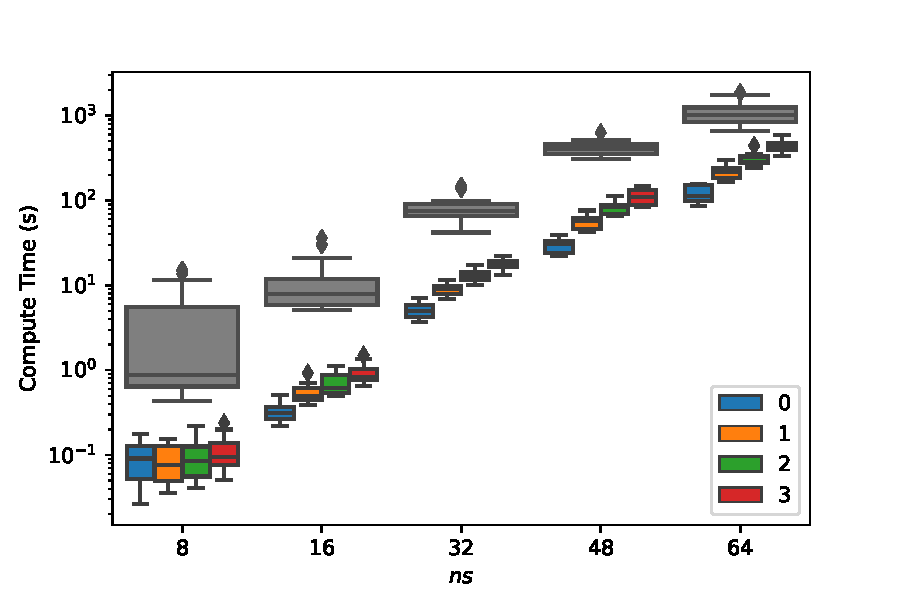
\includegraphics[width=5in]{compute_time_violin}
  \caption{Computation time required for numerical asymptotics and finite difference algorithms over a range of spatial grid sizes using 32 CPUs. Only five grid sizes are shown, with the finite difference and numerical asymptotic algorithm for $n=0,\ldots,3$ terms shown for each grid. The horizontal offset within each grid size is only for visual clarity. TODO: Replace violin plots with box--and--whisker plots.}
  \label{fig:compute_time_violin}
\end{figure}

%Figure \ref{fig:mms_asym_err_time_collapsed} shows the error incurred in the asymptotic approximation versus the computation required for a several values of $b$ and $n$ in order to give a sense of the trade--off between speed and accuracy.
%All calculations are perfomed on the same $64 \times 8$ spatial--angular grid, and errors are compared pointwise to the finite difference calculation using the same value of $b$ on the same grid.
%The dashed black line is a linear fit through the computations in $(\ln\left(\varepsilon/b^n\right), \ln t)$ space with slope $m=0.55 \approx 1/2$.
%This demonstrates the approximate relationship between error, scattering coefficient, and number of terms,
%\begin{equation}
%  \varepsilon t^2 \propto b^n.
%\end{equation}
%So, for example, for a given value of $b$, the error incurred by the scattering coefficient can be halved (for suitable values of $b$), but at the expense of approximately quadrupling the computation time.
%\begin{figure}[H]
%  \centering
%  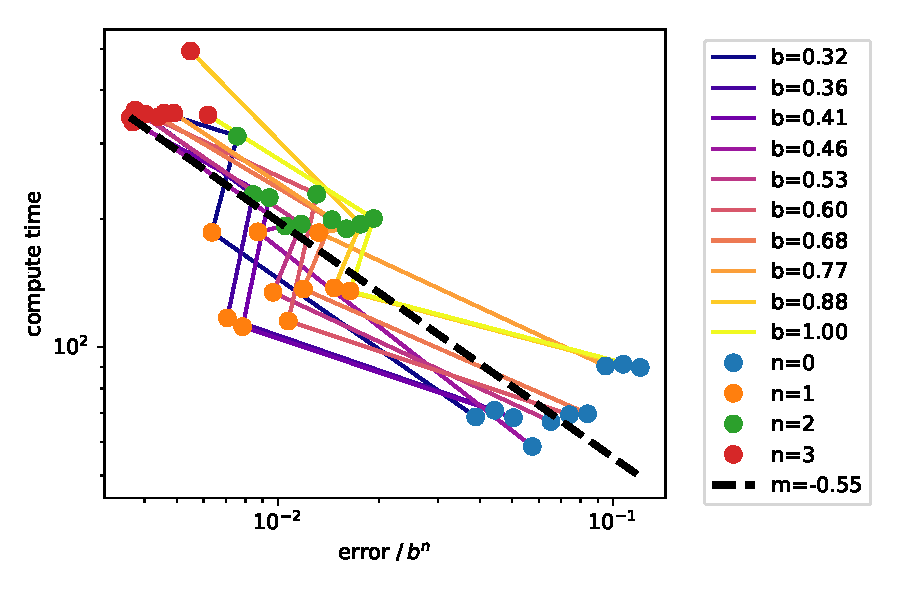
\includegraphics[width=5in]{mms_asym_err_time_collapsed}
%  \caption{To give an idea of the trade--off between accuracy and speed; $n_s=64$, $n_a=8$. . 32 cores.}
%  \label{fig:mms_asym_err_time_collapsed}
%\end{figure}

\subsection{Memory Usage}
Memory usage is perhaps the most important consideration when choosing the algorithm and grid size.
While the numerical asymptotics algorithm requires only a few multiples of the memory required to store the radiance itself, the finite difference algorithm requires the generation and storage of a coefficient matrix several orders of magnitude larger than the solution vector.
These memory requirements are given for a combination of spatial and angular grid sizes in Table \ref{tab:mem_store}.
It is worth noting that using several terms from the asymptotic series does not increase the memory usage, as the same arrays are reused between iterations.

Furthermore, the actual iterative solution of the matrix equation requires the allocation of several multiples of that amount of memory.
A good approximation of the memory required to solve the linear system with GMRES (restarted every 100 iterations) is five times the memory required to store the coefficient matrix.
Even for large grids, the numerical asymptotics has not been observed to use more than five gigabytes of memory, which is well within the memory capacity of a common modern laptop or workstation.
On the other hand, the finite difference algorithm uses enormous amounts of memory, from tens of gigabytes for small to medium grids, and hundreds of gigabytes for large grids.
These estimates are plotted in Figure \ref{fig:mem_solve}, and listed numerically in Table \ref{tab:mem_solve}.
\begin{figure}[H]
  \centering
  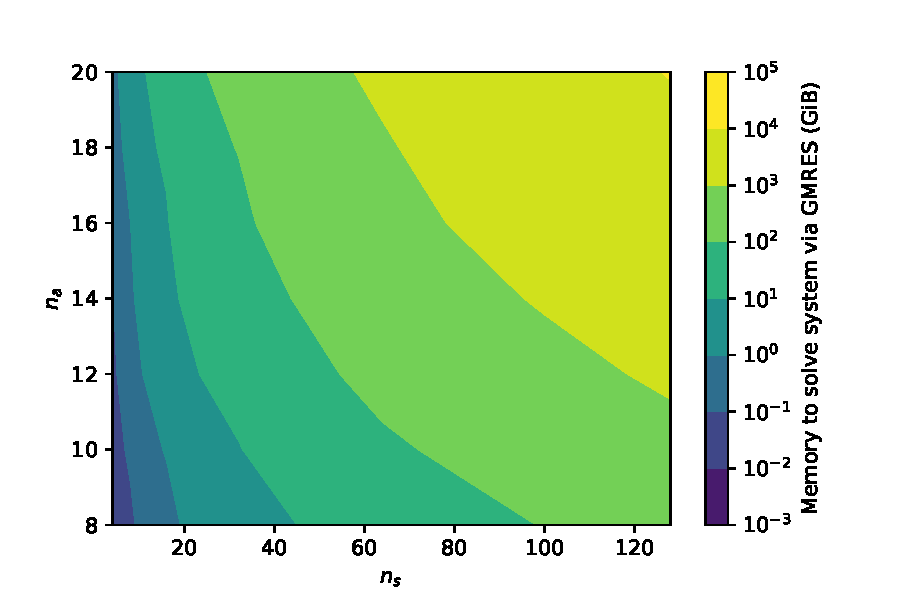
\includegraphics[width=5in]{memory_solve}
  \caption{Estimated memory required to solve the linear system of equations for the finite difference algorithm using GMRES, restarted every 100 iterations. Table \ref{tab:mem_solve} contains the same data in text form.}
  \label{fig:mem_solve}
\end{figure}

%\section{Grid Size and Discretization Error}
\section{Optical Conditions for Asymptotics}
Since the asymptotic approximation is based on a Taylor series expansion around the case of no scattering, it is only valid for relatively small scattering coefficients.
Extremely high--scattering scenarios are out of reach for the asymptotic approximation, and the finite difference approach must be used in those cases.
Whereas in low--scattering waters, adding terms to the asymptotic series tends to decrease the error in the solution, in high--scattering situations, adding terms causes the error to diverge.
Therefore, if the finite difference solution is out of the question for cases of high scattering, the leading order approximation is the best option.
An in--depth analysis of the error incurred by the numerical asymptotics algorithm is presented in this Section.

\subsection{Raw Simulation Results}
\label{sec:iop_study_raw}
In all of the following results, the properties of the kelp are held constant while the optical properties of the water are varied.
Ten values of $a_w$ are taken at equal intervals on a linear scale from \SI{0.1}{\per\m} to \SI{0.5}{\per\m} (inclusive), and ten values of $b$ are taken at even intervals on a log scale from \SI{0.01}{\per\m} to \SI{1.5}{\per\m} (inclusive).
For each set of optical properties, numerical asymptotics is employed with 0, 1, 2, and 3 scattering events, and a finite difference calculation is performed.
A spatial--angular grid size of $72 \times 10$ is used for all calculations.
Each asymptotics calculation is compared to the finite difference calculation with the same optical properties, and a pointwise error is calculated.
Figure \ref{fig:asym_real_kelp_br01} shows this type of comparison for a single value of $a_w$, varying $b$.
As discussed in Section \ref{sec:num_asym_mms}, the order $n$ approximation converges with roughly order $n+1$.
However, the Figure shows that this trend does not continue indefinitely as $b$ decreases.
This is because although the truncation error is decreasing, the discretization error is remaining constant.
Therefore, no results with this grid size will show errors below about \SI{0.01}{\W\per\m\squared\per\radian}.
As a result, simulations with errors below this threshold in order to gain insight into trends in truncation error.

\newcommand\rdfigwidth{4.5in}

\begin{figure}[H]
  \centering
  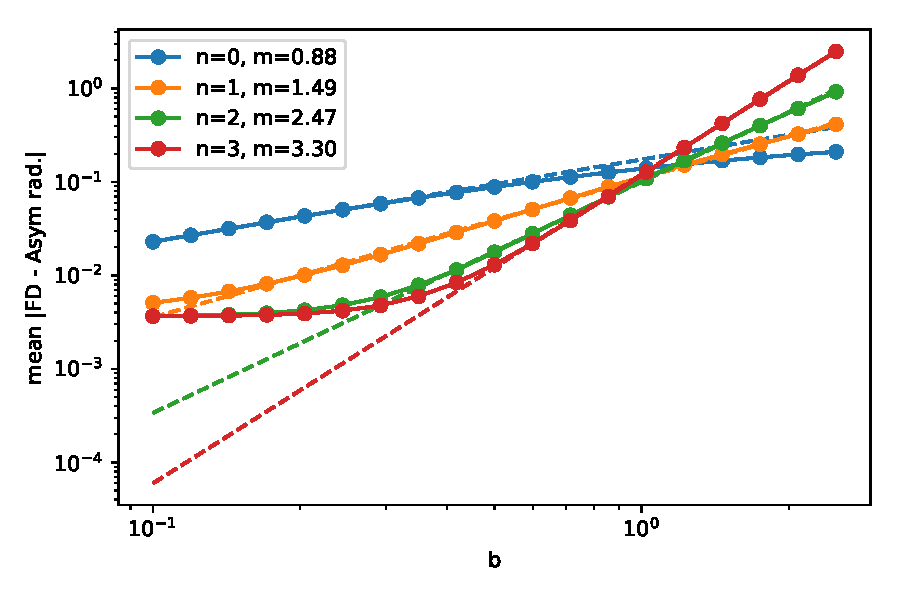
\includegraphics[width=\rdfigwidth]{verify_real_kelp_asym_b_scat_ss_sm_th_a05_br01_72x10_rad_err}
  \caption{Asym real kelp. Blur radius=0.1}
  \label{fig:asym_real_kelp_br01}
\end{figure}

Figure \ref{fig:asym_err_vs_ab} shows a different slice of the simulation results.
Here, $n=0$ is held constant while $a_w$ and $b$ are plotted on the $x$ and (log) $y$ axes, with average error plotted on the (log) color scale.
Note that mean error does not depend only on $b$.
Rather, errors are largest for waters with low absorption and high scattering, and lowest for low scattering, high absorption.
The clear pattern in the variation of error over the $a_w$--$b$ domain indicates that a third parameter can be calculated sufficiently from $a_w$ and $b$ which is sufficient to determine the accuracy of the approximation.

\begin{figure}[H]
  \centering
  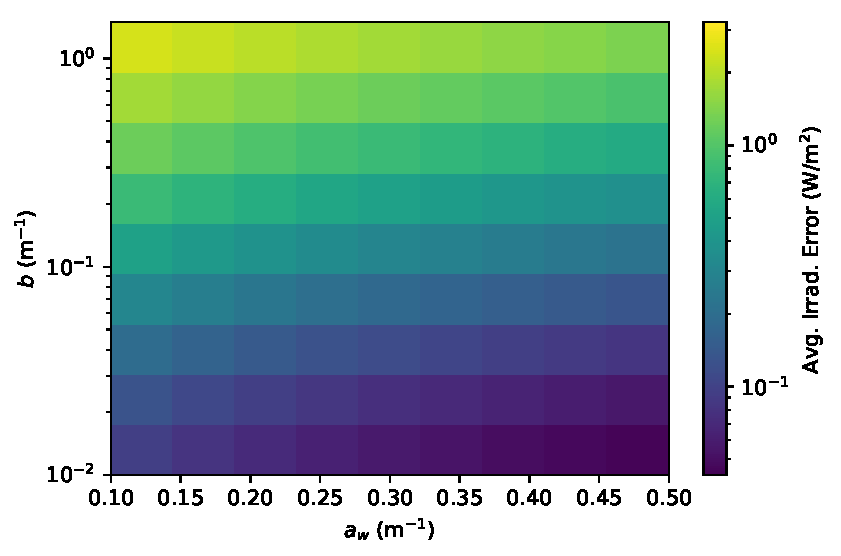
\includegraphics[width=\rdfigwidth]{asym_err_vs_ab}
  \caption{asym err vs ab}
  \label{fig:asym_err_vs_ab}
\end{figure}

Figure \ref{fig:best_n_data_vs_ab} shows a similar view of the simulation results as Figure \ref{asym_err_vs_ab}, except that now, the different approximation orders are considered for each set of optical properties, and the order with the lowest error is found.
The order of the best approximation is shown for each case, and the error incurred by that approximation is shown on the color axis.
In the upper left corner, the most difficult cases are shown.
In this region, the zeroth order approximation is most accurate, showing that additional terms cause the solution to diverge.
After a brief transition region, the third order approximation is most accurate, in agreement with Figure \ref{fig:asym_real_kelp_br01}.

Note that for low scattering, high absorption waters where the error is lowest, the second order approximation seems to perform better than the third order.
As mentioned previously, this is because a lower bound on the total error is imposed by the discretization error, as suggested by Figure \ref{fig:asym_real_kelp_br01}.
In fact, the second and third order approximations are nearly identical; the former is only slightly better, and no conclusions about truncation error should be drawn from this part of the figure.

\begin{figure}[H]
  \centering
  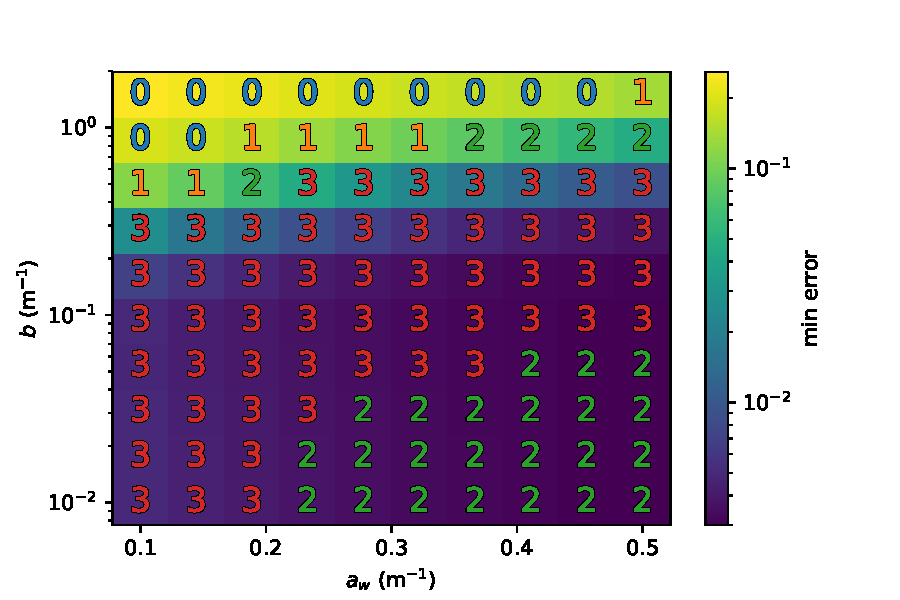
\includegraphics[width=\rdfigwidth]{best_n_data_vs_ab}
  \caption{best n data vs ab}
  \label{fig:best_n_data_vs_ab}
\end{figure}

In actual usage, one is concerned not with finding the best approximation, but rather the cheapest one which meets some error threshold.
This concept is explored in Figures \ref{fig:min_n_data_vs_ab_eps01}, \ref{fig:min_n_data_vs_ab_eps005}, and \ref{fig:min_n_data_vs_ab_eps001}.
In each Figure, an average error threshold of $\bar{\varepsilon}=\SI{0.1}{\W\per\m\squared\per\radian}$, $\bar{\varepsilon}=\SI{0.05}{\W\per\m\squared\per\radian}$, and $\bar{\varepsilon}=\SI{0.01}{\W\per\m\squared\per\radian}$, respectively is set, and the lowest order approximation to meet the error threshold is shown.
The error of that approximation is shown on the color axis.
In each case, there are some optical properties for which the error threshold cannot be met for any $n$.
This is represented by an ``X'' in the figure, and the error of the leading order approximation is shown in color.
Note that as $\bar\varepsilon$ is decreased, the error threshold cannot be satisfied for a larger set of optical properties, and where it is achievable, more scattering terms are required.

\begin{figure}[H]
  \centering
  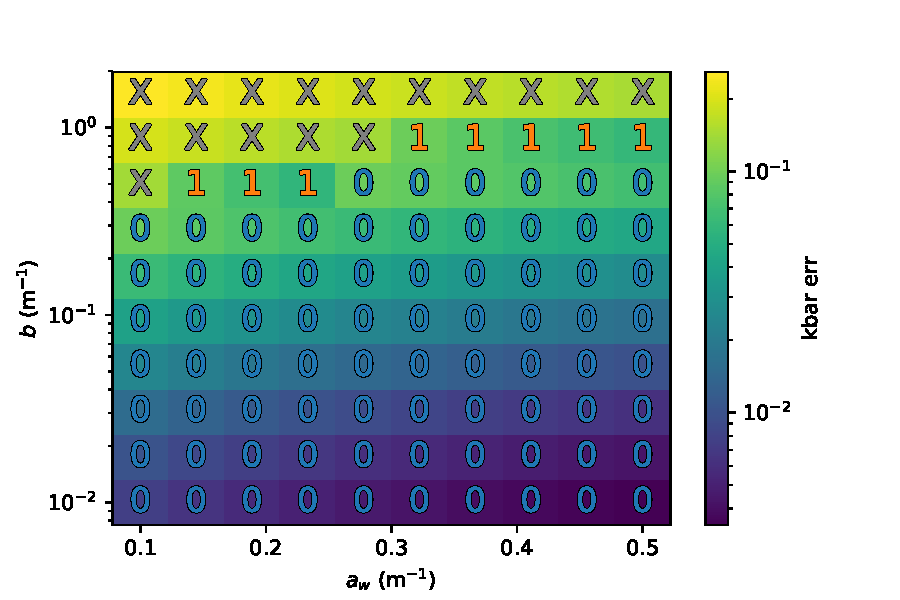
\includegraphics[width=\rdfigwidth]{min_n_data_vs_ab_eps01}
  \caption{min n data vs ab eps01}
  \label{fig:min_n_data_vs_ab_eps01}
\end{figure}

\begin{figure}[H]
  \centering
  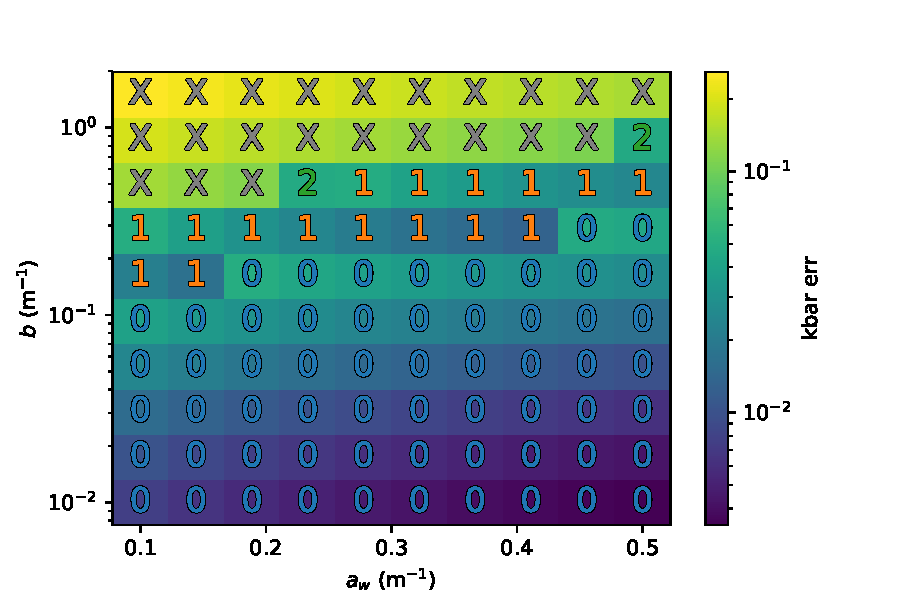
\includegraphics[width=\rdfigwidth]{min_n_data_vs_ab_eps005}
  \caption{min n data vs ab eps005}
  \label{fig:min_n_data_vs_ab_eps005}
\end{figure}

\begin{figure}[H]
  \centering
  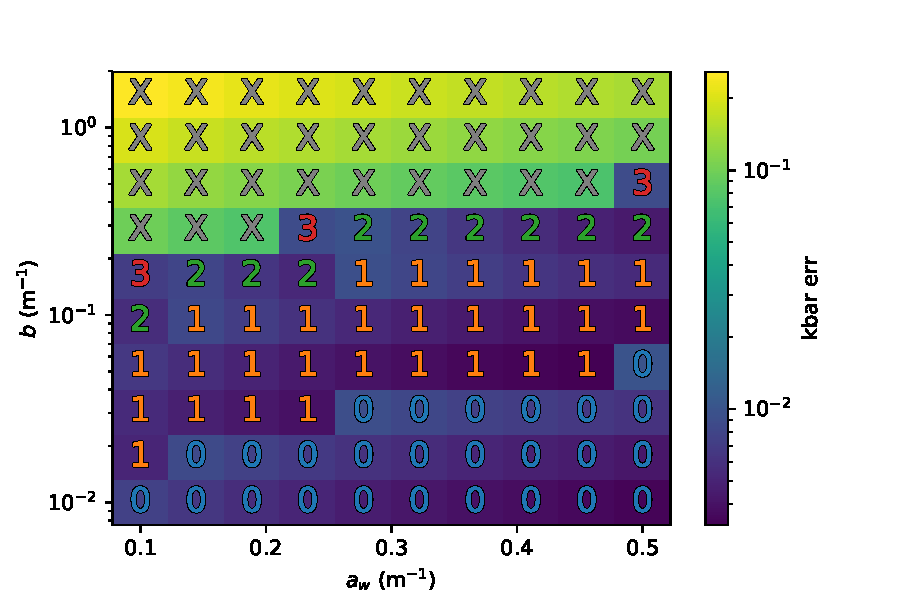
\includegraphics[width=\rdfigwidth]{min_n_data_vs_ab_eps001}
  \caption{min n data vs ab eps001}
  \label{fig:min_n_data_vs_ab_eps001}
\end{figure}

\subsection{Error Model}
Figure \ref{fig:asym_err_data_xi_model} concisely represents the simulation results for all optical properties and all approximation orders, with error $\varepsilon$ plotted on the vertical axis and $b$ plotted on the color axis.
In the left column, $a_w$ is plotted on the horizontal axis.
On a log--log--log scale, the simplicity of the relationship between these three quantities is striking.
Holding $b$ constant, a log--log linear relationship is apparent between the error $\varepsilon$ and the absorption coefficient $a_w$.
Meanwhile, holding $a_w$ constant, log--uniform increases in $b$ cause log--constant increases in $\varepsilon$.
That is, $\ln\varepsilon$ seems to increase linearly with $\ln b$ and decrease linearly with $\ln a$.
Restated, it seems that
\begin{equation}
  \varepsilon \propto \frac{b^{c_1}}{a_w^{c_2}}.
\end{equation}

Then, by fitting a plane to the observed values in $(\ln a_w, \ln b, \ln \varepsilon)$ space, a continuous model can be derived for $\varepsilon(a_w, b)$.
Performing this procedure separately for each $n$ value yields values of $c_1$ and $c_2$ which appear to be independent of $n$.
Remarkably, the fit for each order of approximation yields $c_1=3/4$, $c_2=1/2$ to within a few percent variation.
The black ``x''s in Figure \ref{fig:asym_err_data_xi_model} are the predictions of this model, setting $c_1=3/4$ and $c_2=1/2$ explicitly.
Notice how accurately the observed errors are predicted by the model.
This also suggests the definition of a third parameter, as mentioned in Section \ref{sec:iop_study_raw},
\begin{equation}
  \xi = \frac{b^{3/4}}{a_w^{1/2}},
\end{equation}
with the unusual units \SI{}{\m^{-1/4}}.
In the right column of Figure \ref{fig:asym_err_data_xi_model}, $\varepsilon$ is plotted as a function of $\xi$.
Notice that all of the results collapse onto a single line.
Thus, for the sake of understanding the usefulness of the asymptotic series in approximating the true light field, $\xi$ can be used as a single variable to characterize all waters.

\begin{figure}[H]
  \centering
  %\vspace{-1em}
  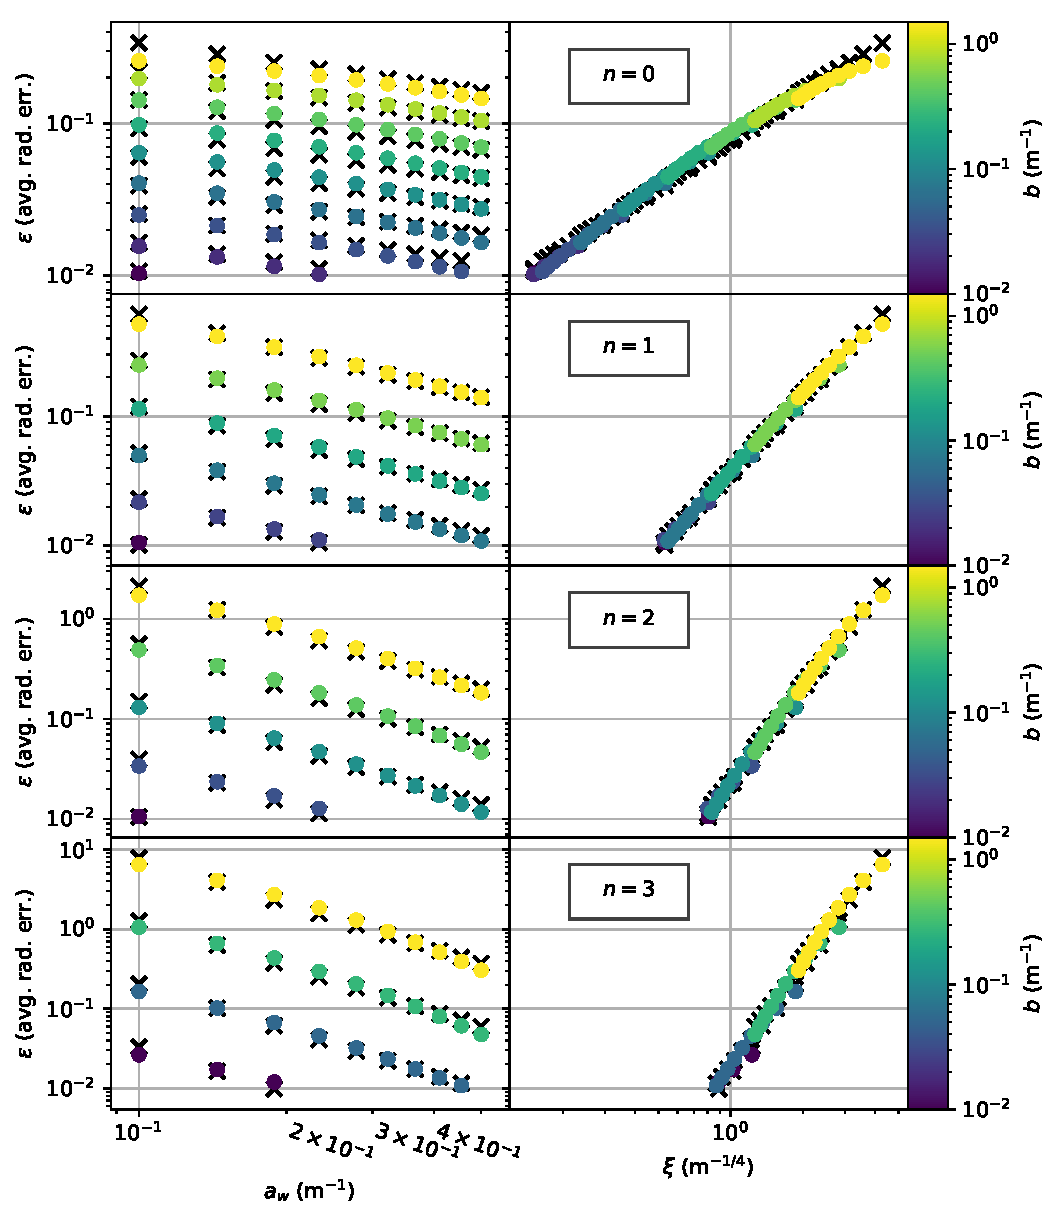
\includegraphics[width=6in]{asym_err_data_xi_model}
  %\vspace{-1em}
  \caption{asym err data $\xi$ model}
  \label{fig:asym_err_data_xi_model}
\end{figure}

In Figure \ref{fig:asym_err_vs_xi_all_n_fit_all}, $\varepsilon$ is plotted as a function of $\xi$ for all combinations of $a_w$, $b$, and $n$, effectively combining the right column of Figure \ref{fig:asym_err_data_xi_model} on a single plot.
For each $n$, the log--log plot displays a clear linear relationship, similar to the pattern seen previously in Figures \ref{fig:asym_real_kelp_br01} and \ref{fig:mms_asym_b_conv}.
However, this figure abstracts that pattern over both $a_w$ and $b$, whereas previously it was seem only for $b$.
Note that the convergence curves for all lines appear to roughly intersect at a characteristic point.
That point, denoted $(\xi^*, \varepsilon^*)$, is significant because it represents a bifurcation in the convergence behavior of the numerical asymptotics algorithm.
For waters with $\xi < \xi^*$, adding terms to the series increases the accuracy of the approximation, whereas for waters with $\xi$ above the threshold value $\xi^*$, adding terms decreases the accuracy.

In order to systematically determine $(\xi^*, \varepsilon^*)$, the log--log convergence curve of order $n+1$ is assumed to have slope $n+1$, which is approximately true, at least for $\xi<\xi^*$.
Further, it is assumed that there is a single point where all of these curves intersect.
This point fully specifies the convergence curves, all other free parameters having been eliminated by the previous assumptions.
Thus, the error for the order $n$ approximation satisfies
\begin{equation}
  \label{eqn:ln_eps_n}
  \ln\varepsilon_n(\xi) - \ln\varepsilon^* = (n+1)\left(\ln\xi - \ln\xi^*\right),
\end{equation}
or equivalently,
\begin{equation}
  \label{eqn:eps_n}
  \varepsilon_n(\xi) = \varepsilon^* \left(\frac{\xi}{\xi^*}\right)^{n+1}.
\end{equation}

Then, a residual function is constructed which accumulates squared differences between the fit functions and their corresponding data points, weighting all squared errors by $1/\varepsilon$ in order to deem the runs with lower errors more important since errors diverge for large $\xi$ values and do not fit the linear function quite as well.
A numerical optimization algorithm is then used to search the two dimensional parameter space for the minimizers of the residual, which produces the point $(\xi^*, \varepsilon^*)$.
This procedure yields the result
\begin{align}
  \xi^* &= 1.63, \\
  \varepsilon^* &= 0.11,
\end{align}
shown in Figure \ref{fig:asym_err_vs_xi_all_n_fit_all}.
Thus, waters characterized below this threshold are worth considering for solution via numerical asymptotics, whereas others are better suited for a finite difference solution.

\begin{figure}[H]
  \centering
  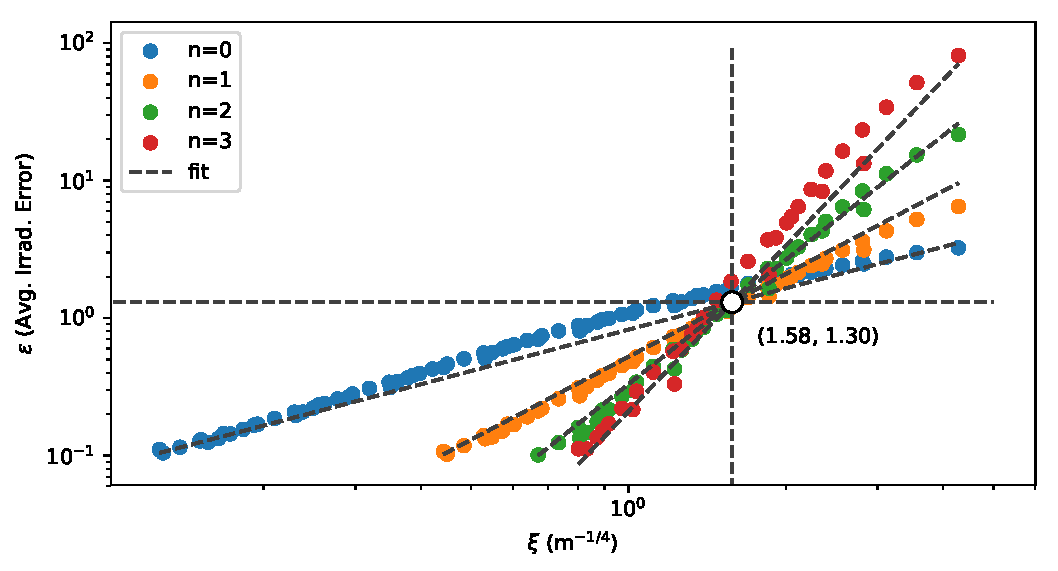
\includegraphics[width=5in]{asym_err_vs_xi_all_n_fit_all}
  \caption{asym err vs xi all n fit all}
  \label{fig:asym_err_vs_xi_all_n_fit_all}
\end{figure}

The determination of $\xi^*$ and $\varepsilon^*$ marks the construction of a simple analytical model given by Equation \ref{eqn:eps_n} which predicts the errors for any set of aquatic optical properties.
Figure \ref{fig:asym_err_model_vs_ab_all_k} shows the predictions of this model for several values of $a_w$, $b$, and $n$, with $\varepsilon$ plotted on the color axis.
Note that $\xi^*$ is a contour in $(a_w, b)$ space, and is marked on the figure with a dashed white line.
$\xi<\xi^*$ is the region to the lower right of the threshold, and $\xi>\xi^*$ is the region to the upper left.
Also keep in mind that this model and its predictions deal only with truncation error, and that discretization error distorts the actual solution accuracy, as seen in Figures \ref{fig:asym_real_kelp_br01} and \ref{fig:best_n_data_vs_ab}.

\begin{figure}[H]
  \centering
  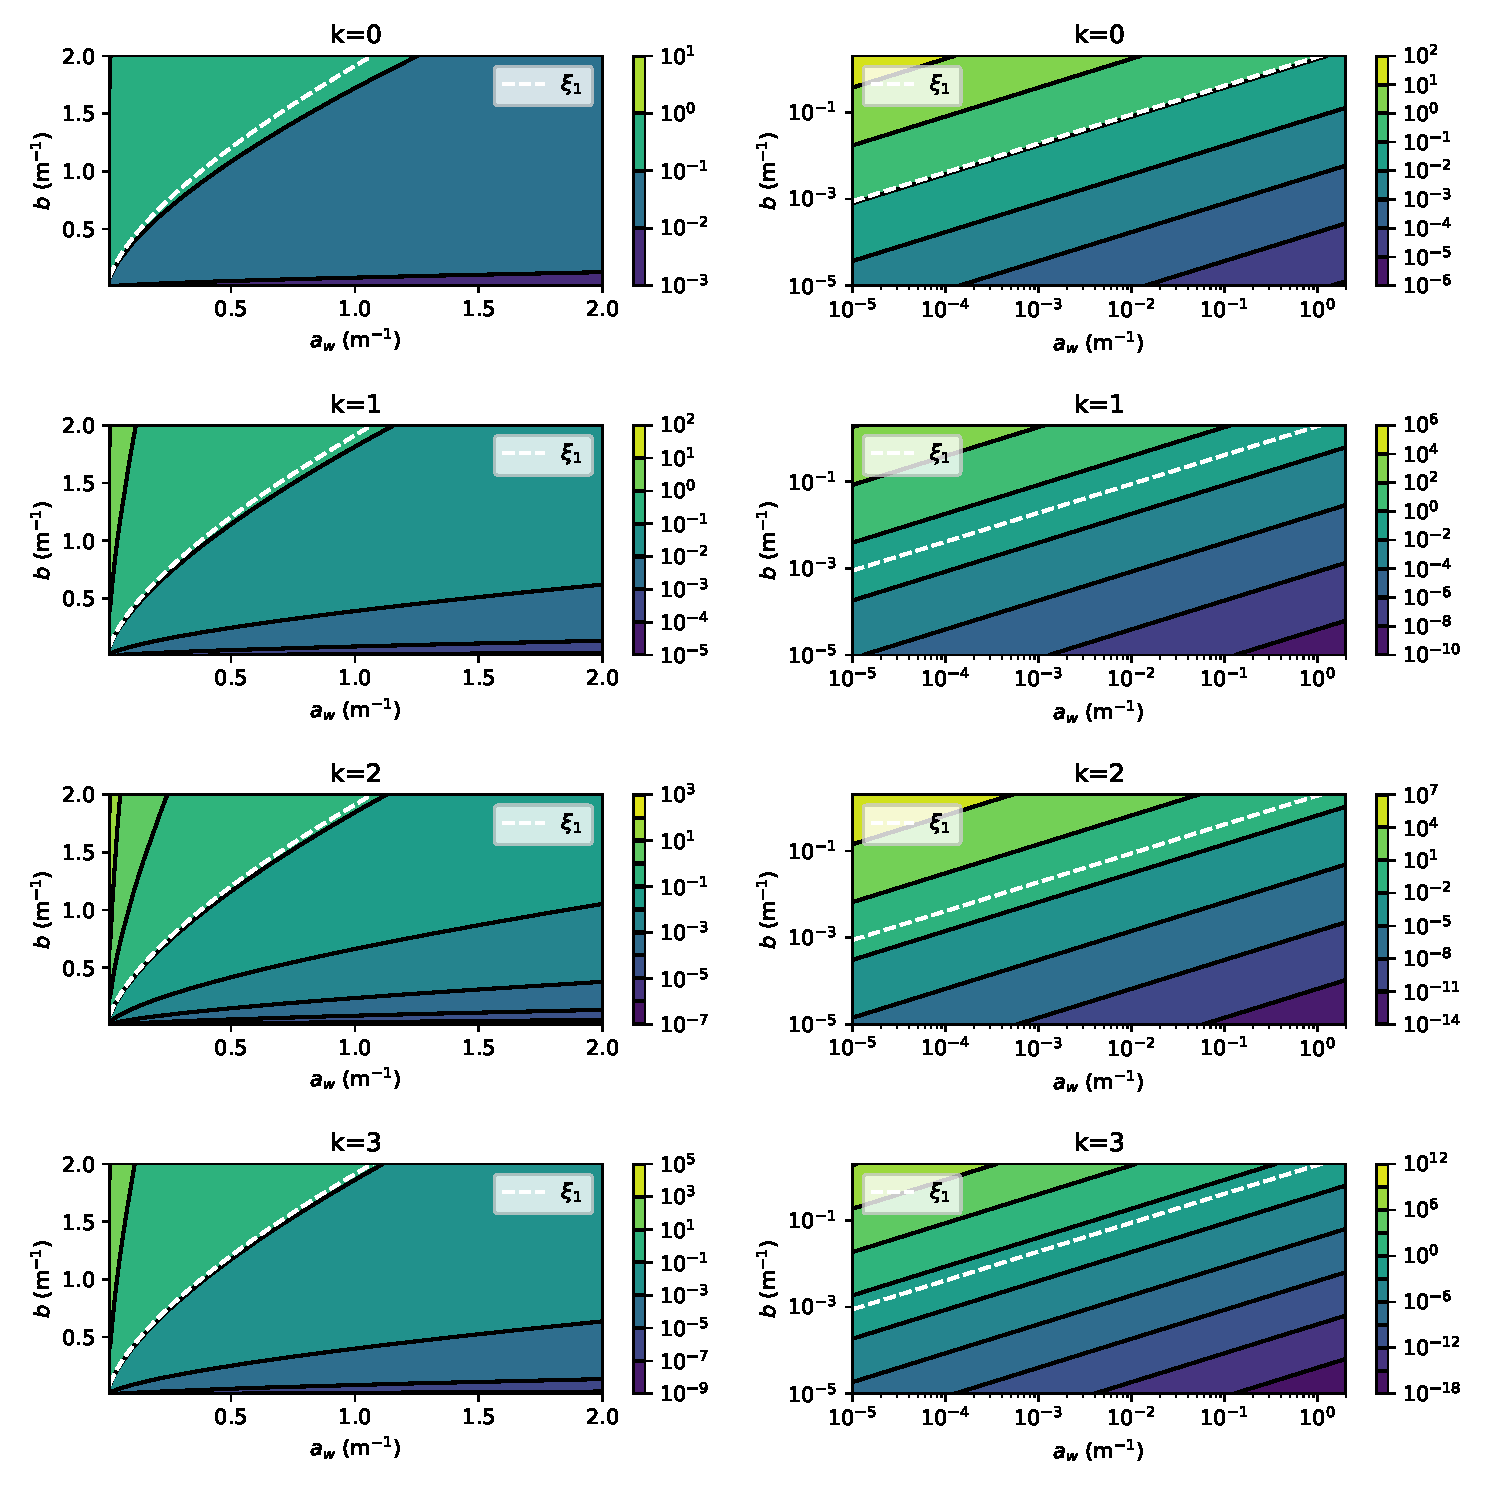
\includegraphics[width=5in]{asym_err_model_vs_ab_all_k}
  \caption{asym err model vs ab all k}
  \label{fig:asym_err_model_vs_ab_all_k}
\end{figure}

This model can now be used to produce general guidelines for the choice of $n$ given a desired error.
Assuming that a maximum error $\varepsilon=\bar\varepsilon$ is permissible, the minimum order of $n$ which produces $\varepsilon$ is desired.
This order, denoted $\bar{n}$, can determined by solving Equation \ref{eqn:ln_eps_n} for $n$ when $\varepsilon=\bar{\varepsilon}$ and rounding up to the nearest integer.
That is,
\begin{equation*}
  \bar{n} = \ceil\left(\frac{\ln\bar{\varepsilon} - \ln\varepsilon^*}{\ln\xi - \ln\xi^*} - 1 \right),
\end{equation*}
which is equivalent almost everywhere to
\begin{equation}
  \label{eqn:n_bar}
  \bar{n} = \floor\left(\frac{\ln\bar{\varepsilon} - \ln\varepsilon^*}{\ln\xi - \ln\xi^*}\right).
\end{equation}

Figure \ref{fig:nbar_model_vs_ab_3eps} shows $\bar{n}$ up to $\bar{n}=3$ for $\bar{\varepsilon}=0.1$, $\bar{\varepsilon}=0.05$, and $\bar{\varepsilon}=0.01$.
The $\xi^*$ contour is plotted.
Assuming that $\bar{\varepsilon}<\varepsilon^*$, if higher contours of $\bar{n}$ were plotted, they would approach the $\xi^*$ contour as $\bar{n} \to \infty$ since no accuracy better than $\varepsilon^*$ is achievable by any order approximation when $\xi > \xi^*$.

To summarize this analysis, once an error threshold $\bar{\varepsilon}$ is chosen, the optical properties $a_w$ and $b$ determine the optimal numerical approach according to Figure \ref{fig:nbar_model_vs_ab_3eps} and Equation \ref{eqn:n_bar}.
If $\xi^*(a_w, b) > \xi^*$, then the finite difference algorithm should be used if possible.
If memory or computation time requires the numerical asymptotics algorithm to be used, then the $n=0$ approximation should be used, effectively ignoring scattering.

If $\bar{n}>3$ (i.e., the gray region between $\xi^*$ and $\bar{n}=3$), it is theoretically possible to achieve the desired accuracy in this region by continuing to add terms, however, this is not recommended since the closer $\xi$ is to $\xi^*$, the more likely it is that higher order terms will cause the solution to diverge due to some unexpected deviation in the actual performance of the algorithm from the theoretical error model presented here.
As a compromise, $n=2$ or $n=3$ could be used in this region to balance the severity of divergence in the case of failure with the improved accuracy of the solution in the case of successful convergence.
Finally, in any of the easier regions defined by $\bar{n} \leq 3$, the optimal trade--off between accuracy and computation time is achieved by using $n=\bar{n}(a_w, b)$.

\begin{figure}[H]
  \centering
  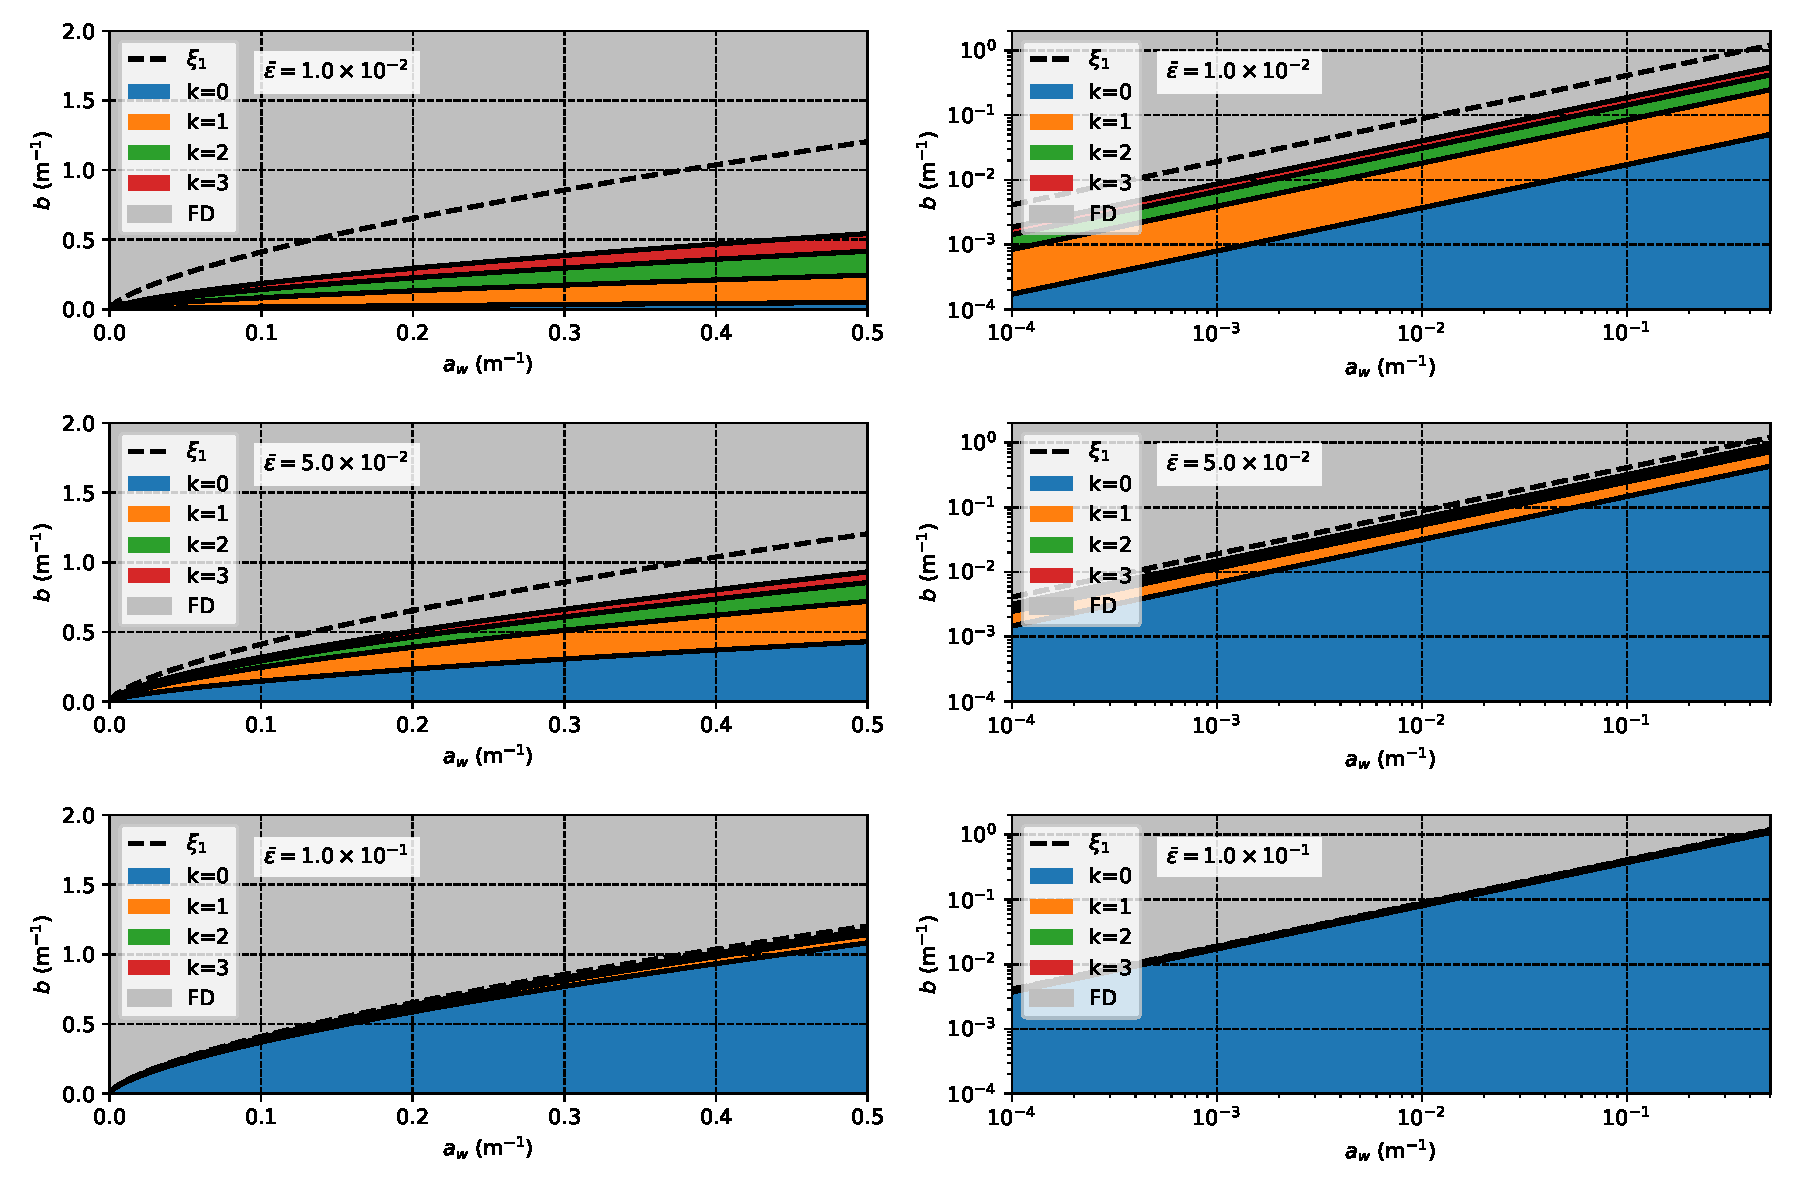
\includegraphics[width=5in]{nbar_model_vs_ab_3eps}
  \caption{nbar model vs ab 3eps}
  \label{fig:nbar_model_vs_ab_3eps}
\end{figure}


\section{Comparison to Other Light Models}

Now that recommendations have been given for the choice of solution method, with the computational cost and accuracy of each having been discussed, all that remains is to compare the solutions obtained from the model presented in this thesis to other available models for the light field.
Two very simple models are used; in both cases, the number of calculations can be counted on two hands, whereas the model of this thesis involves many millions of calculations.
Whether the insight gained from the more complex model is worth the computational expense depends on the purpose of the calculation, and is the decision for the reader to make according to their best judgment for the situation.

\subsection{Simpler Models}
The first model is the simplest conceivable light model --- exponential attenuation with a constant absorption coefficient $a=a_w$.
That is, the simplest solution is to ignore the kelp entirely.
Of course, a depth--dependent absorption coefficient is likely to be used in a real simulation, but for the sake of the comparison, a constant $a_w$ is used.
The irradiance in this case is simply
\begin{equation}
  I(z) = \exp\left(-a_w z \right).
\end{equation}

The second light model, presented in \citep{broch_modelling_2012}, accounts for the kelp by adding a depth--dependent term to the absorption coefficient related to the area and spatial density of the seaweed.
The model is described by
\begin{align}
  \frac{dI}{dz} &= -\left(a_w + k_{\mbox{kelp}}(z)\right),
  \label{eqn:exp_kelp_dIdz}\\
  k_{\mbox{kelp}}(z) &= -\ln(1-A_k(1-(1-AD)^{\rho_n(z)})),
  \label{eqn:exp_kelp_k}
\end{align}
where $A_k$ is the kelp absorptance, $D$ is the number of vertical kelp ropes per horizontal \SI{}{\m\squared}, $A(z)$ is the average area of the kelp fronds per meter vertical rope, and $\rho_n$ is the number of kelp fronds per vertical meter of rope.
Then,
\begin{equation}
  D = \frac{1}{\left(\xmax-\xmin\right) \left(\ymax-\ymin\right)},
\end{equation}
and the mean frond $A$ is calculated from the mean frond length according to Equation \ref{eqn:area-from-length} as 
\begin{equation}
  A = \frac{{\mu_l}^2}{2f_r}.
\end{equation}

Once $k_{\mbox{kelp}}(z)$ is calculated according to Equation \ref{eqn:exp_kelp_k}, then the solution of Equation \ref{eqn:exp_kelp_dIdz} is a simplified version of Equation \ref{eqn:asymptotics_ode_0} with $\tilde{a}(z)=a_w+k_{\mbox{kelp}}(z)$ and $\tilde{\sigma}_0=0$.
The solution is therefore the analogous simplification of Equation \ref{eqn:asymptotics_soln_0}, namely
\begin{equation}
  I(z) = I_0 \exp\left(-a_wz - \int_0^z k_{\mbox{kelp}}(z')\, dz' \right).
\end{equation}

\subsection{Comparison Results}
In Figures \ref{fig:compare_models_n1}, \ref{fig:compare_models_n2}, and \ref{fig:compare_models_n3}, the light model of this thesis is compared to simpler models under the conditions described in Section \ref{sec:standalone_context}.
In the figures, the first model described in this Chapter, which ignores the kelp entirely, is plotted with a black dashed line.
The second model, which uses an additional term in the absorption coefficient to describe the kelp, is plotted with a dashed blue line.
The no--scattering numerical asymptotics solution is plotted in solid red.
Since the above two models do not consider scattering, both the finite difference and asymptotic solutions are plotted for a range of $b$ values, with the finite difference $b$ described by the left color bar, and the asymptotic $b$ described by the right color bar, so as to distinguish between the two sets of curves.

In each of the three Figures, a different value of $n$ is used for the asymptotic approximations for $b>0$: $n=1$, $n=2$, and $n=3$ for Figures \ref{fig:compare_models_n1}, \ref{fig:compare_models_n2}, and \ref{fig:compare_models_n3} respectively. 
In the left column of each figure, the average irradiance is plotted as a function of depth for each of the calculations from the light model of this thesis, calculated over the entire horizontal domain.
In the right column, the perceived irradiance, as described in Section \ref{sec:perceived_irrad}, is shown for the asymptotics and finite difference calculations.

First, note that the no--kelp model predicts the highest light levels throughout the domain, as should be expected since it ignores a significant aspect of the light reduction.
The simple kelp model agrees with the no--kelp model at the surface, but then reduces more quickly once the kelp, which is largest at $z=2$, is introduced.
At the bottom of the domain where there is little kelp remaining, the two curves are seen to be parallel in the log--linear scale, showing that the absorption coefficients are equal as at the surface.
Looking at the left column, the average irradiance from no--scattering solution to the 3D model appears to agree quite well with the simple kelp model, especially near the surface and bottom, where both models are approximately reduced to the first model.
In the $z=2$ region where the most kelp is present, the 3D model predicts higher absorption than the simpler 1D model.
However, between $z=3$ and $z=4$, the 3D kelp model decreases more slowly than the 1D model, perhaps because light is able to penetrate the water in regions where the kelp is not present, and the multitude of angles in which the light travels allow some of the rays to reach even the lower depths without being absorbed by the kelp.

As for the right column, the perceived irradiance is clearly much lower than the average irradiance and the other models.
This makes sense, as the light is dimmest in the regions of highest kelp density, and the perceived irradiance weights these regions the highest, practically ignoring the edges of the domain where light is absorbed only by the water; these regions skew the average irradiance upward although they are not actually representative the light field where photosynthesis is occurring.
From this point of view, it seems that the other two light models significantly overestimate the amount of light available where it actually matters.

Considering the finite difference solution, the most visible effect of increasing scattering is to decrease the light field towards the bottom of the domain.
Of course, scattering does not cause that light to be lost entirely.
Rather, it tends to reflect it towards the surface, where increases in scattering lead to higher light levels.
This is noteworthy since the light available very close to the surface is significantly higher than it is a few meters below.
This tendency for scattering to insulate the upper region of the water may prove to be important in understanding how photosynthesis near the ocean's surface differs from photosynthesis at greater depths.


\begin{figure}[H]
  \centering
  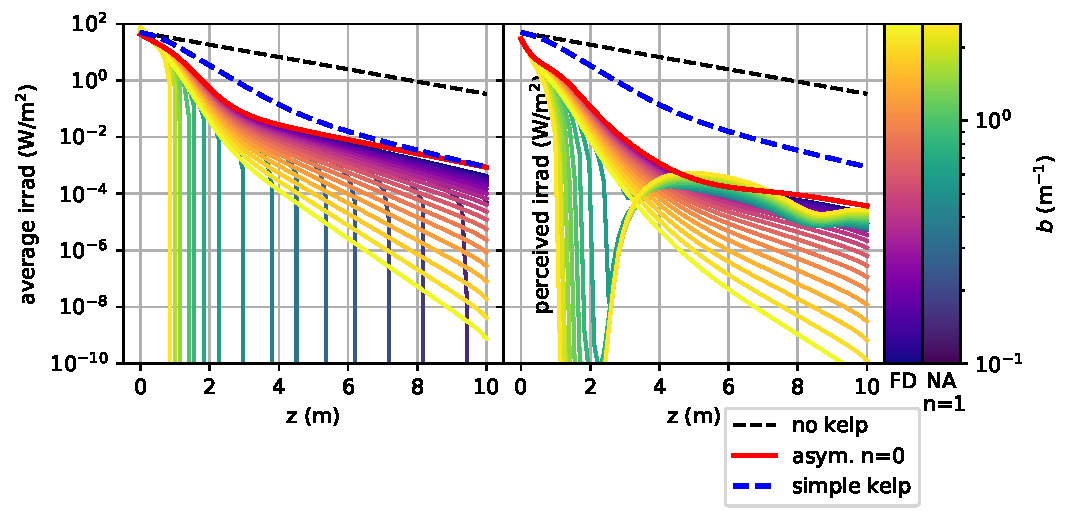
\includegraphics[width=6in]{compare_models_n1}
  \caption{Compare models n=1}
  \label{fig:compare_models_n1}
\end{figure}
\begin{figure}[H]
  \centering
  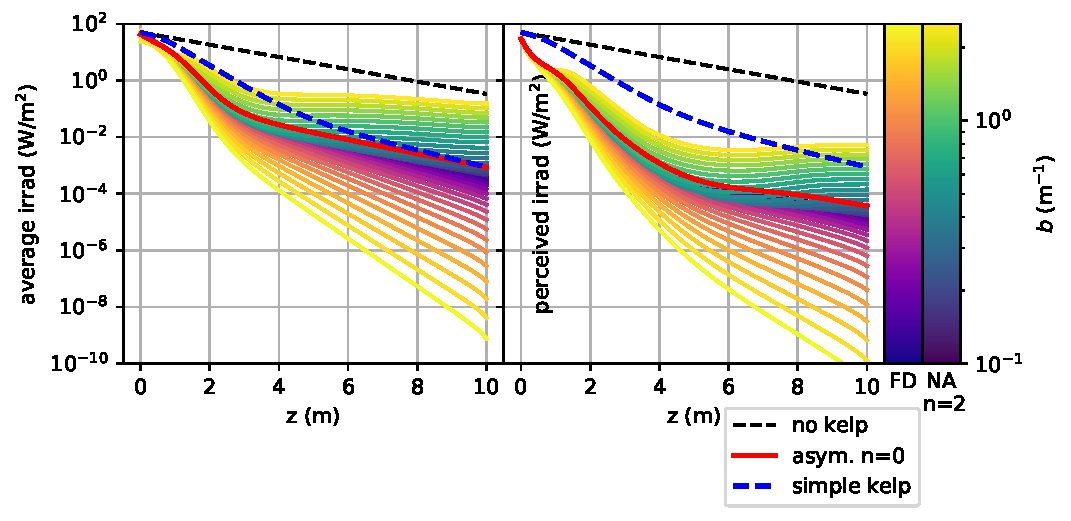
\includegraphics[width=6in]{compare_models_n2}
  \caption{Compare models n=2}
  \label{fig:compare_models_n2}
\end{figure}
\begin{figure}[H]
  \centering
  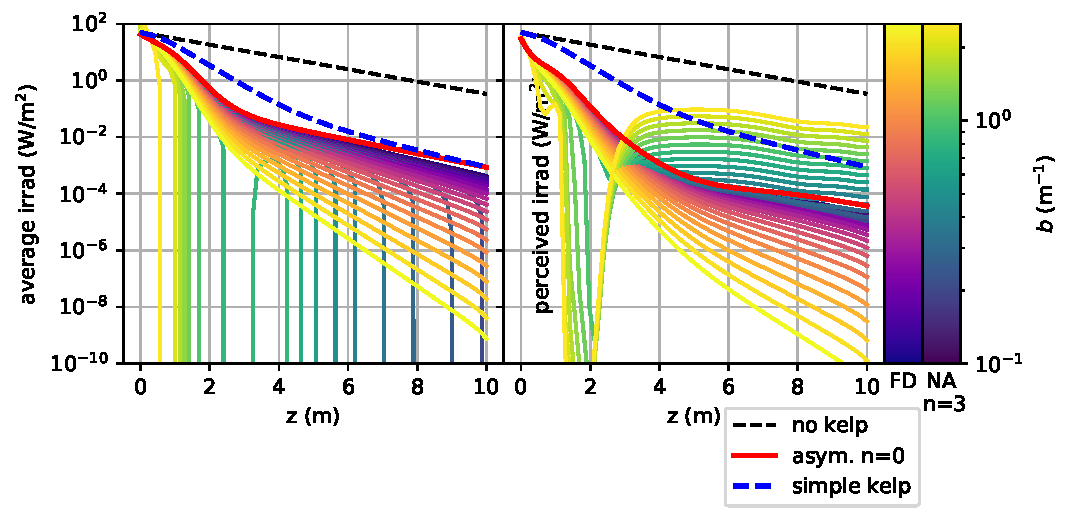
\includegraphics[width=6in]{compare_models_n3}
  \caption{Compare models n=3}
  \label{fig:compare_models_n3}
\end{figure}

\chapter{CONCLUSION}
\label{chap:conclusion}

% TODO: Write this
We present a probabilistic model for the spatial distribution of kelp, and develop a first-principles model for the light field, considering absorption and scattering due to the water and kelp.
A full finite difference solution is presented, and an asymptotic approximation based on discrete scattering events is subsequently developed.

Future work:
\begin{itemize}
  \item Frond bending
  \item Horizontal kelp ropes (long lines)
  \item etc.
  %TODO: Add more
\end{itemize}

\bibliographystyle{abbrv}
\bibliography{bio}
%If you have n appendices, then use the \appendices{n} command below
%followed by n \input{filename} commands, similar to the \input{chapx}
%commands above.
% DO NOT USE SECTIONS OR SUBSECTIONS IN AN APPENDIX OR APPENDICES
\appendix{5}
\chapter{GRID DETAILS}
\label{chap:grid_details}

The width of the spatial grid cells in each dimension are
\begin{align*}
  dx &= \frac{x_{\max}-x_{\min}}{n_x}, \\
  dy &= \frac{y_{\max}-y_{\min}}{n_y}, \\
  dz &= \frac{z_{\max}-z_{\min}}{n_z}.
\end{align*}
and the cell centers as
\begin{align*}
  x_i &= (i-1/2)dx \mbox{ for } i=1,\ldots,n_x, \\
  y_j &= (j-1/2)dy \mbox{ for } j=1,\ldots,n_y, \\
  z_k &= (k-1/2)dz \mbox{ for } k=1,\ldots,n_z.
\end{align*}
Denote the edges as
\begin{align*}
  x_i^e &= (i-1)dx \mbox{ for } i=1,\ldots,n_x, \\
  y_j^e &= (j-1)dy \mbox{ for } j=1,\ldots,n_y, \\
  z_k^e &= (k-1)dz \mbox{ for } k=1,\ldots,n_z.
\end{align*}

Note that in this convention, there are the same number of edges and cells,
and edges precede centers.

Now, we define the azimuthal angle such that
\begin{align*}
  \theta_l = (l-1)d\theta.
\end{align*}
For the sake of periodicity, we need
\begin{align*}
  \theta_1 &= 0, \\
  \theta_{n_\theta} &= 2\pi-d\theta,
\end{align*}
which requires
\begin{equation*}
  d\theta = \frac{2\pi}{n_\theta}.
\end{equation*}
For the polar angle, we similarly let
\begin{equation*}
  \phi_m = (m-1)d\phi.
\end{equation*}
Since the polar azimuthal is not periodic, we also store the endpoint, so
\begin{align*}
  \phi_1 &= 0, \\
  \phi_{n_\phi} &= \pi.
\end{align*}
This gives us
\begin{align*}
  d\phi &= \frac{\pi}{n_\phi-1}.
\end{align*}
It is also useful to define the edges between angular grid cells as
\begin{alignat}{3}
  \theta_l^e &= (l-1/2) d\theta, &\quad l&=1,\ldots,n_\theta \\
  \phi_m^e &= (m-1/2) d\phi, &\quad m&=1,\ldots,n_\phi-1.
\end{alignat}

\begin{figure}[h]
  \centering
  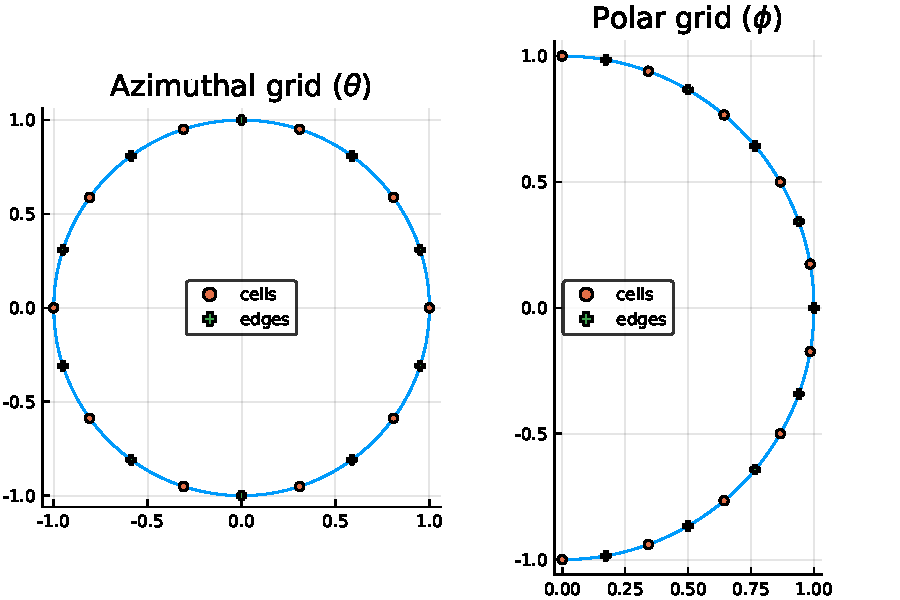
\includegraphics[width=.75\linewidth]{angular_grid_plots}
  \caption{Angular grid cell centers and edges.}
  \label{fig:angular_grid_plots}
\end{figure}

Note that while $\theta$ has its final edge following its final center, this is
not the case for $\phi$, as seen in Figure \ref{fig:angular_grid_plots}.
Because angles are indexed by a single integer $p$, there is a one--to--one relationship between
an integer $p$ and a pair $(l,m)$.
The relationships are
\begin{align*}
  \hat{l}(p) &= \mbox{mod1}(p, n_\theta), \\
  \hat{m}(p) &= \ceil(p/n_\theta) + 1, \\
  p &= \left( \hat{m}(p)-2\right)n_\theta + \hat{l}(p).
\end{align*}
Accordingly, define
\begin{align*}
  \hat{\theta}_p &= \theta_{\hat{l}(p)}, \\
  \hat{\phi}_p &= \phi_{\hat{m}(p)}, \\
  \hat{p}(l,m) &= (m-1)n_\theta + l.
\end{align*}

We refer to the angular grid cell centered at $\vec{\omega}_p$ as $\Omega_p$, and the solid angle subtended by $\Omega_p$ is denoted $\abs{\Omega_p}$.
The areas of the grid cells are calculated as follows.
Note that there is a temporary abuse of notation in that the same symbols ($d\theta$ and $d\phi$) are being used for infinitesimal differential and for finite grid spacing.
For the poles, we have
\begin{align*}
  \abs{\Omega_1} = \abs{\Omega_\nomega} &= \int_{\Omega_1} d{\vec{\omega}} \\
  &= \int_0^{2\pi}\int_0^{d\phi/2} \sin\phi\, d\phi\, d\theta \\
  &= 2\pi \cos\phi \Big|_{d\phi/2}^0 \\
  &= 2\pi(1-\cos(d\phi/2)).
\end{align*}
For all other angular grid cells,
\begin{align*}
  \abs{\Omega_p} &= \int_{\Omega_p} d{\vec{\omega}} \\
                 &= \int_{\theta_l^e}^{\theta_{l+1}^e}\int_{\phi_m^e}^{\phi_{m+1}^e} \sin(\phi)\, d\phi\, d\theta \\
                 &= d\theta \int_{\phi_m^e}^{\phi_{m+1}^e} \sin(\phi)\, d\phi \\
                 &= d\theta\left( \cos(\phi_m^e)-\cos(\phi_{m+1}^e) \right).
\end{align*}

\chapter{SYNTHETIC DATA}
\label{chap:synthetic_data}

In order to perform code verification via the Method of Manufactured solutions, analytical functions for radiance, absorption coefficient, and volume scattering function must be chosen which are simple to evaluate, are differentiable, and satisfy the constraints imposed by the algorithm implementation that are listed in Section \ref{sec:synthetic_data}.
The functions chosen to meet the above conditions are
\begin{align}
  L(x, y, z, \theta, \phi) &=
    \alpha \left(\sin{\left (\phi + \theta \right )} + 1\right) \nonumber\\
    &\quad\cdot \left(z \left(\sin{\left (\frac{2 \pi x}{\alpha} \right )} + \sin{\left (\frac{2 \pi y}{\alpha} \right )}\right) + 1\right) \nonumber\\
    &\quad\cdot \left(- \gamma + z + \frac{\tanh{\left (\left(b + 1\right) \left(\gamma - z\right) \right )}}{\tanh{\left (\gamma \left(b + 1\right) \right )}}\right),
  \label{eqn:mms_sol_expr} \\
  a(x, y, z) &= \sin{\left (\frac{2 \pi x}{\alpha} \right )} + \sin{\left (\frac{2 \pi y}{\alpha} \right )} + \tanh{\left (- \gamma + z \right )} + 5,
  \label{eqn:mms_abs_expr} \\
  \beta(\Delta) &= \frac{\Delta + 1}{4 \pi},
  \label{eqn:mms_vsf_expr}
\end{align}
where $\alpha=x_{max}-x_{min}=y_{max}-y_{min}$ is the domain width, and $\gamma=z_{max}-z_{min}$ is the domain depth.
Using the python package Sympy \cite{meurer_sympy:_2017}, the boundary conditions and source function are calculated to be
\begin{align}
  &\quad\qquad f(\theta, \phi) = \alpha \left(- \gamma + 1\right) \left(\sin{\left (\phi + \theta \right )} + 1\right),
  \label{eqn:mms_bc_expr} \\
  &\sigma(x, y, z, \theta, \phi) = \alpha \left(z \left(\sin{\left (\frac{2 \pi x}{\alpha} \right )} + \sin{\left (\frac{2 \pi y}{\alpha} \right )}\right) + 1\right) \left(\sin{\left (\phi + \theta \right )} + 1\right) \nonumber\\
  %
  &\quad \cdot \left(- \gamma + z + \frac{\tanh{\left (\left(b + 1\right) \left(\gamma - z\right) \right )}}{\tanh{\left (\gamma \left(b + 1\right) \right )}}\right) \left(b + \sin{\left (\frac{2 \pi x}{\alpha} \right )} + \sin{\left (\frac{2 \pi y}{\alpha} \right )} + \tanh{\left (- \gamma + z \right )} + 5\right) \nonumber\\
  %
  &\quad - b \Bigg[ \frac{\alpha \left(z \left(\sin{\left (\frac{2 \pi x}{\alpha} \right )} + \sin{\left (\frac{2 \pi y}{\alpha} \right )}\right) + 1\right) \left(\frac{\sin{\left (\phi \right )} \sin{\left (\theta \right )}}{3} + \frac{\cos{\left (\phi \right )}}{3}\right) \left(- \gamma + z + \frac{\tanh{\left (\left(b + 1\right) \left(\gamma - z\right) \right )}}{\tanh{\left (\gamma \left(b + 1\right) \right )}}\right)}{4 \pi} \nonumber\\
  %
  &\quad - \frac{\alpha \left(z \left(\sin{\left (\frac{2 \pi x}{\alpha} \right )} + \sin{\left (\frac{2 \pi y}{\alpha} \right )}\right) + 1\right) \left(- \gamma + z + \frac{\tanh{\left (\left(b + 1\right) \left(\gamma - z\right) \right )}}{\tanh{\left (\gamma \left(b + 1\right) \right )}}\right)}{4 \pi} \nonumber\\
  %
    &\quad \cdot \left(-\frac{\pi \sin{\left( \phi \right)}\sin{\left( \theta \right)}}{2} - \frac{\sin{\left (\phi \right )} \sin{\left (\theta \right )}}{3} - \frac{\cos{\left (\phi \right )}}{3}\right) \nonumber\\
  %
  &\quad - \frac{\alpha \left(z \left(\sin{\left (\frac{2 \pi x}{\alpha} \right )} + \sin{\left (\frac{2 \pi y}{\alpha} \right )}\right) + 1\right) \left(- \gamma + z + \frac{\tanh{\left (\left(b + 1\right) \left(\gamma - z\right) \right )}}{\tanh{\left (\gamma \left(b + 1\right) \right )}}\right)}{4 \pi} \nonumber\\
  %
    &\quad \cdot \left(\frac{\sin{\left( \phi \right)}\sin{\left( \theta \right)}}{3} - \frac{2 \pi \sin{\left (\phi \right )} \cos{\left (\theta \right )}}{3} + \frac{\cos{\left (\phi \right )}}{3} - 2 \pi\right) \nonumber\\
  %
  &\quad + \frac{\alpha \left(z \left(\sin{\left (\frac{2 \pi x}{\alpha} \right )} + \sin{\left (\frac{2 \pi y}{\alpha} \right )}\right) + 1\right) \left(- \gamma + z + \frac{\tanh{\left (\left(b + 1\right) \left(\gamma - z\right) \right )}}{\tanh{\left (\gamma \left(b + 1\right) \right )}}\right)}{4 \pi} \nonumber\\
  %
  &\quad \cdot \left(- \frac{\pi \sin{\left (\phi \right )} \sin{\left (\theta \right )}}{2} - \frac{\sin{\left(\phi\right)}\sin{\left(\theta\right)}}{3} + \frac{2 \pi \sin{\left (\phi \right )} \cos{\left (\theta \right )}}{3} - \frac{\cos{\left (\phi \right )}}{3} + 2 \pi\right) \Bigg] \nonumber\\
  %
  &\quad + 2 \pi z \left(\sin{\left (\phi + \theta \right )} + 1\right) \left(- \gamma + z + \frac{\tanh{\left (\left(b + 1\right) \left(\gamma - z\right) \right )}}{\tanh{\left (\gamma \left(b + 1\right) \right )}}\right) \sin{\left (\phi \right )} \sin{\left (\theta \right )} \cos{\left (\frac{2 \pi y}{\alpha} \right )} \nonumber\\
  %
  &\quad + 2 \pi z \left(\sin{\left (\phi + \theta \right )} + 1\right) \left(- \gamma + z + \frac{\tanh{\left (\left(b + 1\right) \left(\gamma - z\right) \right )}}{\tanh{\left (\gamma \left(b + 1\right) \right )}}\right) \sin{\left (\phi \right )} \cos{\left (\theta \right )} \cos{\left (\frac{2 \pi x}{\alpha} \right )} \nonumber\\
  %
  &\quad + \Bigg[\alpha \left(z \left(\sin{\left (\frac{2 \pi x}{\alpha} \right )} + \sin{\left (\frac{2 \pi y}{\alpha} \right )}\right) + 1\right) \nonumber\\
  &\quad \cdot \left(\frac{\left(- b - 1\right) \left(- \tanh^{2}{\left (\left(b + 1\right) \left(\gamma - z\right) \right )} + 1\right)}{\tanh{\left (\gamma \left(b + 1\right) \right )}} + 1\right) %\nonumber\\
  %
  \left(\sin{\left (\phi + \theta \right )} + 1\right) \nonumber\\
  %
  &\quad + \alpha \left(\sin{\left (\frac{2 \pi x}{\alpha} \right )} + \sin{\left (\frac{2 \pi y}{\alpha} \right )}\right) \left(\sin{\left (\phi + \theta \right )} + 1\right) \nonumber\\
  &\quad \cdot \left(- \gamma + z + \frac{\tanh{\left (\left(b + 1\right) \left(\gamma - z\right) \right )}}{\tanh{\left (\gamma \left(b + 1\right) \right )}}\right)\Bigg] \cos{\left (\phi \right )}.
  \label{eqn:mms_source_expr}
\end{align}

\chapter{MEMORY USAGE}
\label{chap:memory_usage}

The matrix size in memory in bytes is calculated as follows.
\begin{lstlisting}[language=Python]
def calc_size(ns, na):
    nx = ns
    ny = ns
    nz = ns
    ntheta = na
    nphi = na
    nomega = ntheta * (nphi-2) + 2

    nnz = nx * ny * nomega * ( nz * (6 + nomega) - 1)

    return 8*nnz
\end{lstlisting}

Memory requirement for LIS solution via GMRES with restart=100 is well-estimated by multiplying the above by 5.

\begin{sidewaysfigure}
  \centering
  \caption{Memory to store one copy of the finite difference coefficient matrix}
  \begin{tabular}{llllllll}
  \toprule
  {} &          8  &          10 &          12 &          14 &          16 &          18 &          20 \\
  \midrule
  4   &    1.36 MiB &    3.51 MiB &    7.61 MiB &   14.59 MiB &   25.57 MiB &   41.88 MiB &      65 MiB \\
  8   &   10.91 MiB &   28.15 MiB &   60.94 MiB &  116.79 MiB &   204.7 MiB &  335.17 MiB &   520.2 MiB \\
  16  &    87.4 MiB &  225.34 MiB &  487.76 MiB &  934.67 MiB &     1.6 GiB &    2.62 GiB &    4.06 GiB \\
  32  &  699.61 MiB &    1.76 GiB &    3.81 GiB &     7.3 GiB &    12.8 GiB &   20.95 GiB &   32.52 GiB \\
  48  &    2.31 GiB &    5.94 GiB &   12.87 GiB &   24.65 GiB &    43.2 GiB &   70.73 GiB &  109.76 GiB \\
  64  &    5.47 GiB &   14.09 GiB &    30.5 GiB &   58.43 GiB &   102.4 GiB &  167.65 GiB &  260.18 GiB \\
  72  &    7.78 GiB &   20.06 GiB &   43.42 GiB &    83.2 GiB &   145.8 GiB &   238.7 GiB &  370.45 GiB \\
  100 &   20.86 GiB &   53.76 GiB &  116.34 GiB &  222.91 GiB &  390.63 GiB &  639.54 GiB &  992.51 GiB \\
  128 &   43.74 GiB &  112.74 GiB &  243.99 GiB &  467.48 GiB &  819.22 GiB &    1.31 TiB &    2.03 TiB \\
  \bottomrule
  \end{tabular}
\end{sidewaysfigure}

\begin{sidewaysfigure}
  \centering
  \caption{Memory to solve the linear system of equations with GMRES restarted
every 100 iterations. This seems to require roughly five times the memory required
to store the matrix.}
  \begin{tabular}{llllllll}
  \toprule
  {} &          8  &          10 &          12 &          14 &           16 &          18 &          20 \\
  \midrule
  4   &    6.81 MiB &   17.57 MiB &   38.05 MiB &   72.94 MiB &   127.87 MiB &  209.39 MiB &  325.01 MiB \\
  8   &   54.57 MiB &  140.74 MiB &   304.7 MiB &  583.96 MiB &  1023.51 MiB &    1.64 GiB &    2.54 GiB \\
  16  &  437.01 MiB &     1.1 GiB &    2.38 GiB &    4.56 GiB &        8 GiB &    13.1 GiB &   20.32 GiB \\
  32  &    3.42 GiB &    8.81 GiB &   19.06 GiB &   36.52 GiB &       64 GiB &  104.77 GiB &   162.6 GiB \\
  48  &   11.53 GiB &   29.72 GiB &   64.33 GiB &  123.25 GiB &   215.99 GiB &  353.63 GiB &   548.8 GiB \\
  64  &   27.34 GiB &   70.46 GiB &  152.48 GiB &  292.16 GiB &      512 GiB &  838.24 GiB &    1.27 TiB \\
  72  &   38.92 GiB &  100.32 GiB &  217.11 GiB &  415.99 GiB &      729 GiB &    1.17 TiB &    1.81 TiB \\
  100 &  104.29 GiB &  268.79 GiB &   581.7 GiB &    1.09 TiB &     1.91 TiB &    3.12 TiB &    4.85 TiB \\
  128 &  218.72 GiB &   563.7 GiB &    1.19 TiB &    2.28 TiB &        4 TiB &    6.55 TiB &   10.16 TiB \\
  \bottomrule
  \end{tabular}
\end{sidewaysfigure}

\chapter{RAY TRACING ALGORITHM}
\label{chap:ray_tracing}


In order to evaluate a path integral through the discrete grid, it
is first necessary to construct a one-dimensional piecewise constant integrand
which is discontinuous at unevenly spaced points corresponding to the
intersections between the path and edges in the spatial grid.

Consider a grid center $\vec{p_1} = (p_{1x},p_{1y},p_{1z})$ and a corresponding path $\vec{l}(\vec{x_1}, \vec{\omega}, s)$.
To find the location of discontinuities in the integrand, we first calculate the
distance from its origin, $\vec{p_0} = \vec{x_0}(\vec{p_1}, \vec{\omega}) = (p_{0x}, p_{0y}, p_{0z})$ (as in \eqref{eqn:x_0}) to grid edges in each dimension
separately.
Given
\begin{align}
  x_i &= p_{0x} + \frac{s_i^x}{\tilde{s}}(p_{1x}-p_{0x}), \\
  y_j &= p_{0y} + \frac{s_j^y}{\tilde{s}}(p_{1y}-p_{0y}), \\
  z_k &= p_{0z} + \frac{s_k^z}{\tilde{s}}(p_{1z}-p_{0z}),
\end{align}
the path lengths at which the ray intersects with edges in each dimension are calculated to be
\begin{align}
  s_i^x &= \tilde{s}\frac{x_i-p_{0x}}{p_{1x}-p_{0x}}, \\
  s_i^y &= \tilde{s}\frac{y_i-p_{0y}}{p_{1y}-p_{0y}}, \\
  s_i^z &= \tilde{s}\frac{z_i-p_{0z}}{p_{1z}-p_{0z}}.
\end{align}
We also keep a variable for each dimension specifying whether the ray increases
or decreases in the dimension. Let
\begin{align}
  \delta_x &= \sign(p_{0x}-p_{1x}), \\
  \delta_y &= \sign(p_{0y}-p_{1y}), \\
  \delta_z &= \sign(p_{0z}-p_{1z}).
\end{align}
For convenience, we also store a closely related quantity, $\sigma$ with a value 1 for
increasing rays and 0 for decreasing rays in each dimension
\begin{align}
  \sigma_x = (\delta_x+1)/2, \\
  \sigma_y = (\delta_y+1)/2, \\
  \sigma_z = (\delta_z+1)/2,
\end{align}
simply as a boolean value to track of the ray direction.

For this algorithm, we keep two sets of indices. $(i,j,k)$ indexes the grid
cell, and is used for extracting physical quantities from each cell along
the path.
Meanwhile, $(i^e,j^e,k^e)$ indexes the edges between grid cells, beginning
after the first cell. That is, $i^e=1$ refers not to the plane $x=\xmin$, but to $x=\xmin+dx$.

Let $(i_0, j_0, k_0)$ be the indices of the grid cell containing $\vec{p_0}$.
That is,
\begin{align}
  i_0 &= \ceil\left(\frac{p_{0x}-\xmin}{dx}\right), \\
  j_0 &= \ceil\left(\frac{p_{0y}-\ymin}{dy}\right), \\
  k_0 &= \ceil\left(\frac{p_{0z}-\zmin}{dz}\right).
\end{align}
Then,
\begin{align}
  i_0^e &= i_0 + \sigma_x, \\
  j_0^e &= j_0 + \sigma_y, \\
  k_0^e &= k_0 + \sigma_z.
\end{align}
Now, we calculate the distance from $p_0$ along the path to edges in each dimension.
\begin{align}
  s_i^x = \hat{s}\frac{x_i^e-p_{0x}}{p_{1x}-p_{0x}}, \\
  s_j^y = \hat{s}\frac{y_j^e-p_{0y}}{p_{1y}-p_{0y}}, \\
  s_k^z = \hat{s}\frac{z_k^e-p_{0z}}{p_{1z}-p_{0z}}.
\end{align}

For each grid cell, we check the path lengths
required to cross the next $x$, $y$, and $z$ edge-planes.
Then, we move to the next grid cell in whichever dimension
is crossed soonest.
As each cell is traversed, the absorption coefficient and effective source are saved for use in the ray integral for the numerical calculation of the asymptotic approximation.
For full implementation details, see the \texttt{traverse\_ray} subroutine in \texttt{asymptotics.f90} in Appendix \ref{chap:fortran}.

% Putting it together, we do the following.
% \begin{enumerate}
%   \item Let $i,j,k$ be fixed (denoting the starting grid cell).
%   \item Set $s=0$.
%   \item
% \begin{align}
%   d = \mbox{argmin}_{x,y,z} \left\{ s_i^x-s, s_j^y-s, s_k^z \right\}
% \end{align}
%
% \begin{align}
%   \begin{cases}
%     i = i+\delta_x, & \mbox{if } d=x \\
%     j = j+\delta_y, & \mbox{if } d=y \\
%     z = k+\delta_z, & \mbox{if } d=z
%   \end{cases}
% \end{align}
%
% and
%
% \begin{align}
%   \begin{cases}
%     i^e = i^e+\delta_x, & \mbox{if } d=x \\
%     j^e = j^e+\delta_y, & \mbox{if } d=y \\
%     z^e = k^e+\delta_z, & \mbox{if } d=z
%   \end{cases}
% \end{align}
%
%
% Then, move to the adjacent grid cell in the dimension which requires the shortest
% step to reach an edge. Save $ds$ of the path through this cell. Also save abs.
% coef. and source.
% % TODO: Improve
%
% As the ray traverses the spatial grids, it crosses $N-2$ spatial grid edges.
% Let the nondecreasing path lengths at which these crossings occur be denoted by
% $\left\{s_\nu\right\}_{\nu=1}^{N}$, with the convention $s_1=0$ and $s_{N}=\tilde{s}$.
% This implies that edge $\nu$ preceeds cell $\nu$.
% $\{s_\nu\}$ is not strictly increasing if the ray directly intersects a grid corner,
% which means that multiple edges are traversed at the same path length.
% Hence, the path lengths through the grid cells, indexed by $\nu=1,\ldots,N-1$, are
%
% * TODO *

\chapter{FORTRAN CODE}
\label{chap:fortran}

The full Fortran implementation of the model described in this thesis.
The up--to--date version of this code can be found online at
\texttt{https://github.com/OliverEvans96/kelp}.

utils.f90
\lstinputlisting{utils.f90}

sag.f90
\lstinputlisting{sag.f90}

kelp3d.f90
\lstinputlisting{kelp3d.f90}

rte\_sparse\_matrices.f90
\lstinputlisting{rte_sparse_matrices.f90}

rte3d.f90
\lstinputlisting{rte3d.f90}

kelp\_context.f90
\lstinputlisting{kelp_context.f90}

light\_context.f90
\lstinputlisting{light_context.f90}

asymptotics.f90
\lstinputlisting{asymptotics.f90}

light\_interface.f90
\lstinputlisting{light_interface.f90}


\end{document}
